%Document vide aux normes de l'École nationale des Chartes
%Dernières modifications E. Rouquette (12/2023)

%%%%%%%%%%%%%%%%%%%%%% PRÉAMBULE


%%%%%%%%%%%%%% partie obligatoire du préambule
\documentclass[a4paper,12pt,twoside]{book}
\usepackage{fontspec}
\usepackage{xunicode}
\usepackage[french]{babel}

%%%%%%%%%%%%%%%%%%%%%%%%%%%%%%%%% PACKAGES UTILISÉS

\usepackage{csquotes} % les guillemets français
\usepackage{lettrine} %faire une lettrine (pas obligatoire)

\usepackage[style=enc,sorting=nyt,maxbibnames=10]{biblatex}%charger le style de l'EnC (téléchargeable ici https://ctan.org/pkg/biblatex-enc)
\addbibresource{bibliographie.bib} %le fichier bibliograhique. 

\usepackage{graphicx}
\usepackage{adjustbox}


%RAJOUTEZ ICI VOS PACKAGES

\usepackage{ragged2e} % Pour le texte justifié à gauche
\usepackage{listings}  % Pour l'inclusion de code
\usepackage[table,xcdraw]{xcolor} % Pour la coloration des tableaux et du texte
\usepackage{tabularx} % Pour des tableaux ajustés à la largeur de la page
\usepackage{array} % Pour la gestion des tableaux. Le type de colonne m{}, permet de centrer verticalement le texte dans les cellules.
\usepackage{pdfpages} % Pour inclure des fichiers PDF (annexe 2)
\usepackage{tocbibind} % Pour inclure les annexes dans la table des matières
\usepackage{caption} % Pour les légendes de tableaux et figures
\captionsetup{skip=10pt} % Ajuster l'espacement des légendes


%%%%%%%%%%%%%%%%%%%%%%%%%%%%%%%%% CONFIGURATION DE MISE EN PAGE

%%%%%% Les compteurs (sections, subsections, etc)
\renewcommand{\thesection}{\Roman{section}.}%On ne fait apparaître que le numéro de la section
\renewcommand{\thesubsection}{\arabic{subsection}.}%subsection en chiffres arabes
\renewcommand{\thesubsubsection}{\alph{subsubsection}.}%subsubsection en lettres minuscules
%Si l'on veut faire apparaître les subsubsection dans le table des matières (à commenter sinon)
\setcounter{tocdepth}{3}
\setcounter{secnumdepth}{3}  % La subsubsection (profondeur=3 dans la table des matières) apparait numérotée dans la TdM

%%%%%  Configurer le document selon les normes de l'école

\usepackage[margin=2.5cm]{geometry} %marges
\usepackage{setspace} % espacement qui permet ensuite de définir un interligne
\onehalfspacing % interligne de 1.5
\setlength\parindent{1cm} % indentation des paragraphes à 1 cm

%%%%% Mise en forme des headers (haut de page)

\usepackage{fancyhdr} %package utilisé pour modifier les headers
\pagestyle{fancy} %utiliser ses propres choix de mise en page et non ceux par défaut du package

\setlength\headheight{16pt}%la hauteur des headers
%\renewcommand{\sectionmark}[1]{\markright{\small\textit{\thesection~\  #1}}}%Faire apparaître dans les headers les sections en  petit et en italiques
\renewcommand{\sectionmark}[1]{}%Commenter la lign précédetne et mettre celle-ci pour ne pas avoir le titre des sections dans le header
\renewcommand{\chaptermark}[1]{\markboth{\small\chaptername~\thechapter~--\ \textit{#1}}{}}%idem pour les chapitres
%\renewcommand{\chaptermark}[1]{}%Commenter la ligne précédente et mettre celle-ci pour ne pas avoir le titre des chapitres  dans le header


%%%%%%% Package hyperref
% A mettre après les autres appels de packages car redéfinit certaines commandes).

\usepackage[colorlinks=false, breaklinks=true, pdfusetitle, pdfsubject ={Mémoire TNAH sur l'archivage des photographies nativement numériques aux Archives nationales.}, pdfkeywords={Archivage électronique, Photographie numérique, Paquets d'archives, SIP, Automatisation, Indexation, Signalement}]{hyperref} %
\usepackage[numbered]{bookmark}%va avec hyperref; marche mieux pour les signets. l'option numbered: les signets dans le pdf sont numérotés

%%%%%%%%%%%%%%%%%%%% Package glossaries
\usepackage[toc=true]{glossaries}
\makeglossaries

\newglossaryentry{InterMARC}{%
	name={Standard InterMARC},%
	description={Le standard MARC (acronyme de MAchine-Readable Cataloging), souvent appelé "format MARC", est un standard d'échanges de données bibliographiques qui permet d'assurer l'interopérabilité de ces données entre les différents catalogues numériques adoptant le MARC. L'InterMARC en est une variante française, utilisée principalement par la BnF. Il s'agit de normes de description bibliographiques permettant de déterminer la manière dont les informations décrivant un document sont choisies, organisées et affichées dans un catalogue}}

\newglossaryentry{uml}{%
	name={Unified Modeling Language},%
	description={L'UML est un langage de modélisation graphique, indépendant de tout langage de programmation, qui fournit une méthode normalisée de représentation et de conception dans les domaines du développement logiciel et de la conception orientée objet}}

\newglossaryentry{xml}{%
	name={XML},%
	description={Extensible Markup Language. Langage de balisage conçu pour créer des documents structurés et hiérarchisés à l’aide de balises définies par l'utilisateur, contrairement aux langages de balisage avec des balises prédéfinies. XML est principalement utilisé pour la gestion et l’échange d’informations, permettant de partager et de stocker des données de manière lisible pour les humains et les machines. Son objectif principal est de faciliter l'interopérabilité entre différents systèmes, notamment via Internet}}

\newglossaryentry{openrefine}{%
	name={OpenRefine},%
	description={\href{https://openrefine.org/}{OpenRefine} est un logiciel open source utilisé pour la manipulation et le nettoyage de données. Il permet de structurer, transformer, enrichirn filtrer et corriger des données en masse}}

\newglossaryentry{pronom}{%
	name={PRONOM},%
	description={PRONOM est une base de données développée par les Archives nationales du Royaume-Uni (The National Archives) pour la gestion et la conservation des formats de fichiers numériques. Elle fournit des informations sur les caractéristiques techniques de nombreux formats. PRONOM aide les archivistes à identifier et gérer les formats de fichiers rencontrés afin de mieux les pérenniser}}

\newglossaryentry{csv}{%
	name={CSV},%
	description={Le CSV (Comma-Separated Values) est un format de fichier utilisé pour stocker des données tabulaires sous forme de texte brut. Chaque ligne du fichier représente une ligne de la table, et les valeurs de chaque colonne sont séparées par des virgules (ou par d'autres séparateurs, comme les points-virgules)}}

\newglossaryentry{docstrings}{%
	name={DocStrings},%
	description={En Python, les docstrings (ou chaînes de documentation) sont des chaînes de caractères intégrées directement dans le code source pour documenter les modules, classes, fonctions ou méthodes. Elles sont définies entre triples guillemets (""" ou ''') et fournissent des informations sur le but, le fonctionnement, les paramètres et les valeurs de retour de ces éléments}}

\newglossaryentry{poc}{%
	name={Proof of Concept},%
	description={Une preuve de concept ou POC (proof of concept, en anglais) est une réalisation courte à échelle réduite d'une certaine méthode ou idée pour démontrer sa faisabilité. Il s'agit d'une réalisation initiale, souvent simplifiée, qui permet de vérifier que les concepts théoriques peuvent être appliqués avec succès dans la pratique. Le PoC est utilisé pour évaluer le potentiel et la viabilité d'un projet}}

\newglossaryentry{lto}{%
	name={LTO},%
	description={La bande LTO est un format de stockage sur bande magnétique destiné à l'archivage et à la sauvegarde de grandes quantités de données. Elle a été développée à la fin des années 1990, conjointement par HP, IBM et la division magnetic tape de Seagate. Cette technologie est conçue pour offrir une solution durable de stockage haute capacité}}

\newglossaryentry{python}{%
	name={Python},%
	description={Le langage Python est un langage de programmation open source multi-plateformes et orienté objet. Grâce à des bibliothèques spécialisées, Python s'utilise à la fois pour le développement web, l'analyse de données, l'intelligence artificielle et la gestion d'infrastructures. Actuellement le plus utilisé au monde, ce langage est dit de \enquote{haut niveau} car il permet d'écrire des programmes en utilisant des mots usuels des langues naturelles et des symboles mathématiques familiers}}


%%%%%%%%%%%%%%%%%% DÉFINITION DES COMMANDES ET ENVIRONNMENTS

% Police pour les environnements de code
\DeclareFixedFont{\ttb}{T1}{txtt}{bx}{n}{12} % gras
\DeclareFixedFont{\ttm}{T1}{txtt}{m}{n}{12}  % normal

%Définition de couleurs d'environnements de code
\definecolor{pink}{HTML}{fc4f86}
\definecolor{blue}{HTML}{040ac2}
\definecolor{red}{HTML}{dd0822}
\definecolor{green}{rgb}{0,0.6,0.1}
\definecolor{orange}{HTML}{ff5733}
\definecolor{background}{HTML}{1E1E1E}   
\definecolor{codetext}{HTML}{D4D4D4}     
\definecolor{orange-string}{HTML}{CE9178}
\definecolor{green-comment}{HTML}{6A9955}
\definecolor{yellow}{HTML}{DCDCAA}   
\definecolor{lightblue}{HTML}{4FC1FF}  

% Définition des couleurs de tableaux
\definecolor{pastelblue}{rgb}{0.6,0.8,1.0}
\definecolor{pastelblue-dark}{rgb}{0.4,0.6,0.9}
\definecolor{pastelpink}{rgb}{1.0,0.8,0.8}
\definecolor{pastelpink-dark}{rgb}{0.8,0.6,0.6}
\definecolor{pastelyellow}{rgb}{1.0,1.0,0.8}
\definecolor{pastelyellow-dark}{rgb}{0.8,0.8,0.6}

% Définition des titres de la bibliographie
\defbibheading{generalites}{\subsection*{Généralités}}
\defbibheading{archivage-e-a-aux-archives-nationales}{\subsection*{L'archivage numérique aux Archives nationales}}
\defbibheading{normes-description}{\subsection*{Les normes de description archivistique et d’échange}}
\defbibheading{cadre-juridique}{\subsection*{Le cadre juridique}}
\defbibheading{systemes-archivage}{\subsection*{Les systèmes d’archivage électroniques}}
\defbibheading{outils-archivage}{\subsection*{ Les outils de l’archivage numérique}}
\defbibheading{documentation-vitam}{\subsubsection*{Documentation Vitam}}
\defbibheading{archives-ia}{\subsection*{Archives et intelligence artificielle}}
\defbibheading{instruments-recherche}{\subsection*{Instruments de recherche}}
\defbibheading{notices-producteur}{\subsection*{Notices producteur}}
\defbibheading{sources-bibliographiques}{\subsection*{Sources bibliographiques}}
\defbibheading{gestion-archives}{\section*{La gestion des archives photographiques}}
\defbibheading{traitements-caracteristiques}{\subsection*{Traitements et caractéristiques des images numériques}}
\defbibheading{histoire-sociologie}{\section*{Histoire et sociologie de la pratique photographique}}

% Définition du style pour le code Python
\newcommand\pythonstyle{\lstset{
		language=Python,
		backgroundcolor=\color{background},     % Couleur de fond
		basicstyle=\ttfamily\color{codetext}, % Couleur du texte
		stringstyle=\color{orange-string},     % Couleur des chaînes
		commentstyle=\color{green-comment}\itshape, % Couleur des commentaires
		emphstyle=\color{pink},  % Couleur des fonctions
		emph={create_archive_unit_dir, sub_unit, create_archive_unit_file},  % Liste des fonctions
		emph={[2]item_path, directory, item, sub_archive_unit, data, data_ir, liste_rp, file_unit, contentsub, archiveunit, exif_data_list, match, createdate, dtf}, % Liste des variables
		emphstyle={[2]\color{yellow}},% Couleur des variables
		emph={[3]for, if, or, elif, in},     % Liste de mots clés
		emphstyle={[3]\color{lightblue}},% Couleur des mots clés
		frame=tb,                              % Cadre en haut et en bas
		breaklines=true,                       % Couper les lignes trop longues
		tabsize=4                              % Taille des tabulations
}}

% Définition d'un nouvel environnement pour le code Python
\lstnewenvironment{python}[1][]
{
	\pythonstyle % Appliquer le style de code Python défini
	\lstset{#1}  % Configurer les options de l'environnement 'listings',  #1 est l'argument optionnel passé lors de l'utilisation de l'environnement
}
{}

% Définition du style pour le code XML
\lstdefinelanguage{XML}
{
	basicstyle=\ttfamily, % Style de base pour le texte du code
	morestring=[b]", % Identification des chaînes de caractères entre guillemets doubles
	morestring=[s]{>}{<}, % Identification des chaînes entre '>' et '<' 
	identifierstyle=\color{blue}, % Couleur des noms de balises
	keywordstyle=\color{orange}, % Couleur des mots clés
	commentstyle=\color{green}, % COuleur des commentaires 
	moredelim=[s][\color{red}]{\ }{=}, % Définition des délimiteurs pour les attributs (espaces suivis d'un signe "=")
	stringstyle=\color{orange}, % COuleur des chaînes de caractères
	moredelim=[s][\color{black}]{>}{<}, % Définition des délimiteurs pour les balises (entre '>' et '<') en noir
	showspaces=false,  % Ne pas montrer les espaces
	frame=tb, % Cadre en haut et en bas
	breaklines=true, % Couper les lignes trop longues
	tabsize=2  % Taille des tabulations}
}

% Définition d'un environnement pour le code XML
\lstnewenvironment{xml}
{
	% Applique le style de code XML et défini la police et la taille du texte, permet aux chaînes de casser automatiquement en fin de ligne, 
	\lstset{language=XML, basicstyle=\ttfamily\small, breaklines=true}
}
{}

% Définition d'un style pour le code XML appelé dans le texte
\newcommand\xmlstyle{\lstset{
		language=XML,
		basicstyle=\ttfamily,
		keywordstyle=\color{orange},
		stringstyle=\color{orange},
		identifierstyle=\color{blue},
		commentstyle=\color{green},
		moredelim=[s][\color{red}]{\ }{=},
		moredelim=[s][\color{black}]{>}{<},
}}

% Défintion d'une commande pour le XML appelé dans le texte
\newcommand\xmlinline[1]{{\xmlstyle\lstinline!#1!}}

% Modification de la commande \arraystretch, qui contrôle l'espacement vertical des lignes dans les tableaux pour ajuster la hauteur des cellules
\renewcommand{\arraystretch}{1.5} 

 %%%%%%%%%%%%%% INFORMATIONS POUR LA PAGE DE TITRE
\author{Selma Bensidhoum - M2 TNAH}
\title{Les enjeux de l’automatisation du traitement archivistique des reportages photographiques numériques de la Présidence de la République aux Archives nationales}

%%%%%%%%%%%%%%%%%%%%%% DOCUMENT
\begin{document}
	\begin{titlepage}
		\begin{center}
			
			\bigskip
			
			\begin{large}				
				ÉCOLE NATIONALE DES CHARTES\\
				UNIVERSITÉ PARIS, SCIENCES \& LETTRES
			\end{large}
			\begin{center}\rule{2cm}{0.02cm}\end{center}
			
			\bigskip
			\bigskip
			\bigskip
			\begin{Large}
				\textbf{Selma Bensidhoum}\\
			\end{Large}
		%selon le cas
			\begin{normalsize}
				\textit{diplômée de master}
			\end{normalsize}
			
			\bigskip
			\bigskip
			\bigskip
			
			\begin{LARGE}
				\textbf{Les enjeux de l’automatisation du traitement archivistique des reportages photographiques numériques de la Présidence de la République aux Archives nationales}\\
			\end{LARGE}
			
			\bigskip
			\bigskip
			\bigskip
			\begin{large}
			\end{large}
			\vfill
			
			\begin{large}
				Mémoire 
				pour le diplôme de master \\
				\enquote{Technologies numériques appliquées à l'histoire} \\
				\bigskip
				2024
			\end{large}
			
		\end{center}
	\end{titlepage}

	\thispagestyle{empty}	
	\cleardoublepage
	
\frontmatter

	\chapter*{Résumé}
\medskip Ce mémoire analyse les défis du traitement archivistique des reportages photographiques numériques produits par le service photographique de la Présidence de la République sous la mandature François Hollande. Face à l'énorme volume de données à verser, il aborde l'enjeu de l'automatisation des paquets d'archives pour alléger le travail des agents, tout en explorant les possibilités d'optimisation de l'indexation de ces reportages. Le mémoire détaille les étapes de réflexion, d’analyse, et de développement technique qui ont conduit à l'élaboration d'une méthode automatisée de fabrication de paquets d'archives. L'intérêt spécifique de l'outil développé est de proposer des solutions d'intégration de métadonnées descriptives issues de sources variées, facilitant ainsi l'accès thématique aux photographies après leur intégration dans le système d'archivage électronique des Archives nationales.

\paragraph{Abstract} This thesis analyses the challenges encountered during the archival processing of digital photographic reports produced by the photographic service of the Presidency of the French Republic under François Hollande. Given the vast volume of data to be archived, it addresses the need for automating the creation of archival packages, while also exploring the opportunities provided by digital technologies to enhance the indexing of these reports and the photographs they contain. The thesis details the stages of reflection, analysis, and technical development that led to the creation of an automated method for producing archival packages. The specific value of the developed tool lies in offering solutions for integrating descriptive metadata from various sources, thereby facilitating thematic access to the photographs after their integration into the National Archives' electronic archiving system.
\\
	
	\textbf{Mots-clés:} archivage électronique ; photographie numérique ; paquets d'archives ; SIP ; automatisation ; indexation ; traitement archivistique ; pipeline.
	
	\textbf{Informations bibliographiques:} Selma Bensidhoum, \textit{Les enjeux de l’automatisation du traitement archivistique des reportages photographiques numériques de la Présidence de la République aux Archives nationales}, mémoire de master \enquote{Technologies numériques appliquées à l'histoire}, dir. Emmanuelle Bermès, Émeline Levasseur, École nationale des chartes, 2024.
	
\newpage{\pagestyle{empty}\cleardoublepage}
	
	\chapter*{Remerciements}
	
\lettrine{J}e souhaite avant tout exprimer ma gratitude envers Émeline Levasseur, en tant que tutrice et professeure. Sa patience et sa bienveillance tout au long de ces deux stages, ainsi que sa pédagogie, m'ont permis d'aborder les problèmes rencontrés avec sérénité et de mener ce projet à bien avec confiance et précision. 

Je souhaite également remercier Emmanuelle Bermès pour son aide précieuse, ses encouragements et sa disponibilité tout au long de mon stage et pendant la formation exigeante qui l'a précédé.

Mes remerciements vont aussi à l'ensemble de l'équipe du Département de l'administration des données pour la qualité de leur accueil et leur accompagnement tout au long de mes stages, tant sur les aspects métier que techniques. Une mention particulière va à André Falut pour ses conseils précieux.

Je remercie enfin Françoise Mahé, pour son soutien indéfectible, sa confiance et ses nombreuses relectures, et Charlotte Lamouche, pour son assistance, tant morale que technique.
\newpage{\pagestyle{empty}\cleardoublepage}
	
%%%%%%%%%%%%
% Impression des bibliographies par catégorie
\chapter*{Bibliographie}
\section*{L'archivage électronique}
\printbibliography[heading=generalites, keyword=generalites]
\printbibliography[heading=archivage-e-a-aux-archives-nationales, keyword=archivage-e-a-aux-archives-nationales]
\printbibliography[heading=normes-description, keyword=normes-description]
\printbibliography[heading=cadre-juridique, keyword=cadre-juridique]
\printbibliography[heading=systemes-archivage, keyword=systemes-archivage]
\printbibliography[heading=outils-archivage, keyword=outils-archivage]
\printbibliography[heading=documentation-vitam, keyword=documentation-vitam]
\printbibliography[heading=archives-ia, keyword=archives-ia]
\section*{ Le Service photographique de la Présidence de la République : histoire et description du fonds}
\printbibliography[heading=instruments-recherche, keyword=instruments-recherche]
\printbibliography[heading=notices-producteur, keyword=notices-producteur]
\printbibliography[heading=sources-bibliographiques, keyword=sources-bibliographiques]
\printbibliography[heading=gestion-archives, keyword=gestion-archives]
\printbibliography[heading=traitements-caracteristiques, keyword=traitements-caracteristiques]
\printbibliography[heading=histoire-sociologie, keyword=histoire-sociologie]


	\chapter*{Introduction}	
\markboth{Introduction}{}
\addcontentsline{toc}{chapter}{Introduction}
Dès 1965, dans son essai consacré aux usages sociaux de la photographie, Pierre Bourdieu écrit :
\begin{quotation}
	\enquote{On s’accorde communément pour voir dans la photographie le modèle de la véracité et de l’objectivité : \enquote{Toute \oe{}uvre d’art reflète la personnalité de son auteur, lit-on dans l’Encyclopédie française. La plaque photographique, elle, n’interprète pas. Elle enregistre. Son exactitude, sa fidélité ne peuvent être remises en cause” […] En réalité, la photographie fixe un aspect du réel qui n’est jamais que le résultat d’une sélection arbitraire, et, par là, d’une transcription..}\footcite[p.108]{bourdieuArtMoyenEssai1965}.}
\end{quotation}

Bourdieu exprime ici l'idée que la photographie est largement perçue comme un médium réaliste car produit mécaniquement et offrant donc une représentation objective du réel, indépendante des choix de son auteur, et donc supposément non sujette à interprétation, contrairement aux autres arts graphiques où la \enquote{patte} de l’auteur est beaucoup plus visible. 

La réalité est encore plus complexe, car au-delà de la subjectivité du photographe mise en avant par Bourdieu à la fin de cette citation, il faut prendre en compte aussi celle de l’observateur. Sur la subjectivité inhérente à l'interprétation des photographies, Gisèle Freund écrit dix ans plus tard :

\begin{quotation}
	\enquote{La photographie du chef d'État, porté dans des cortèges et des démonstrations, surplombant des assemblées, ou ornant les bureaux officiels, est pour les uns le symbole du père, pour les autres celui du Grand Frère orwellien. Elle inspire l'amour ou la haine, la confiance ou la peur. Sa valeur intrinsèque réside dans sa puissance d'éveiller des émotions.\footcite[p.205]{freundPhotographieSociete2006}}
\end{quotation}

En effet, une photographie, bien que capturant un instant précis, peut être perçue de multiples façons selon le contexte dans lequel elle est présentée et le point de vue de l'observateur. Les choix faits par le photographe -- comme l'angle de prise de vue, le cadrage, la composition, et même l'instant choisi pour déclencher l'appareil -- influencent profondément la façon dont l'image sera interprétée.

Ces deux citations illustrent le contraste entre la perception populaire de la photographie et sa réalité en tant que médium. Ainsi, le lien de corrélation entre ces idées réside dans cette tension : alors que la photographie est souvent perçue comme une vérité figée, elle possède en réalité une grande malléabilité interprétative. Cette dualité entre la croyance en sa nature objective et son potentiel de manipulation ou de subjectivité rend la photographie à la fois puissante et complexe, car elle peut être utilisée pour véhiculer des messages très divers, parfois même contradictoires, tout en conservant une aura d'authenticité.

Ces spécificités rendent les photographies particulièrement attrayantes pour les médias et les services de communication, tout en constituant une source d'informations extrêmement riche pour les chercheurs. Il est donc essentiel pour les archivistes non seulement de les rendre accessibles, mais aussi de veiller à ce que leur contexte de production soit documenté et restitué avec rigueur. Cette préoccupation n'est certes pas récente, mais se présente aujourd'hui avec une intensité nouvelle en raison de la production exponentielle de photographies nativement numériques et de leur inclusion croissante dans les versements d'archives.

L'objectif de mes deux stages au Département de l'administration des données en 2023 et 2024, était de proposer des méthodes de reprise des reportages de photographies numériques de la Présidence de la République et des services du Premier Ministre en vue de leur versement dans la nouvelle plateforme d'archivage électronique des Archives nationales. En première année, mes activités se sont concentrées sur le développement d'une méthode semi-automatique de reprise des reportages des services du Premier ministre. Mon stage de fin d'étude s'inscrit dans la continuité du premier : j'étais chargée de développer une méthode automatique de fabrication de paquets d'archives pour les reportages de la Présidence de la République. Dans le cadre de ce mémoire, je m'attacherai à présenter les connaissances et compétences que j'ai dû mobiliser et développer afin d'effectuer cette mission. Nous nous intéresserons donc aux enjeux de l'automatisation du traitement archivistique des photographies nativement numériques à travers l'exemple de la reprise des reportages photographiques de la Présidence aux Archives nationales.

Dans un premier temps, nous nous intéresserons au contexte de production des photographies et à leurs caractéristiques matérielles. En effet, le fait qu'il s'agisse d'archives numériques ne nous exempt pas d'une connaissance approfondie des caractéristiques de cette typologie documentaires. Tout comme un archiviste traitant un fonds de parchemins enluminés se doit de connaître le processus de fabrication du support, les encres utilisées et le langage dans lequel l'auteur s'exprime, un archiviste chargé d'un fonds de photographies numériques doit pouvoir expliciter les caractéristiques techniques des fichiers qu'il traite : supports de stockage, structure du train binaire et des pixels, format des fichiers, métadonnées embarqué, et encodage des données textuelles. 

La dimension immatérielle des archives produites par les technologies numériques représente un défi inédit pour les archivistes. Elle impose de se familiariser avec des concepts et des modes de fonctionnement souvent éloignés de ceux propres à l'archivage papier. En outre, l'archivage numérique ne peut se faire de manière aussi \enquote{directe} que l'archivage papier : alors qu'un archiviste peut accéder physiquement et immédiatement à un fonds papier, l'archivage numérique implique l'intermédiation par une interface technologique. Cette interface, qui interprète une partie des données, crée une distance inévitable entre le professionnel et le fonds qu'il traite. Cette situation est d'autant plus complexe que l'archiviste, souvent formé dans les sciences humaines plutôt qu'en informatique, peut ne pas comprendre entièrement le fonctionnement de cette interface, qui est pourtant cruciale pour l'accès aux informations archivées. L'archiviste n'est toutefois pas démunis devant cette différence de forme, puisque les principes fondamentaux de l'archivage sont applicables au contexte numérique. Les enjeux de description, de classement, et de préservation de l'intégrité des fonds s'appliquent en effet à la gestion des fonds de données numériques.

Dans la deuxième partie de ce mémoire, nous explorerons le cadre normatif et institutionnel de l'archivage numérique qui régit les traitements appliqués aux fonds et les méthodes de versement. Nous commencerons par présenter les normes en vigueur qui encadrent le fonctionnement des systèmes d'archivage électronique ainsi que les méthodes pour la création de paquets d'archives numériques. Nous conclurons cette deuxième partie par une présentation du chantier de reprise des données aux Archives nationales, dans lequel s'inscrit le processus de reprise des reportages photographiques de la Présidence. La \enquote{reprise des données} est le processus par lequel des informations, issues de systèmes anciens, sont extraites, transformées, et réintégrées dans un nouveau système. Dans le contexte de l'archivage numérique aux Archives nationales, il s'agit du transfert des données archivées selon la méthode mise en place par le programme Constance vers la nouvelles solution d'archivage électronique développée par Vitam. 

Ces deux premières parties fourniront une vue d'ensemble des contraintes et des enjeux associés à la gestion de ce fonds dans le contexte actuel. Le développement d'une application pour automatiser la reprise des reportages photographiques m'a conduit à examiner les opportunités offertes par les technologies numériques ainsi que les défis techniques liés à l'automatisation des processus modélisés. L'application que j'ai développée fonctionne selon le principe d'un pipeline de données, c'est à dire comme une chaîne de traitement automatisée. Les données, provenant de diverses sources, entrent dans ce pipeline où elles subissent une série d'opérations successives. Chaque étape du processus est conçue pour transformer, nettoyer, ou enrichir les données, de manière à les rendre compatibles et prêtes pour leur destination finale : ici, le système d'archivage électronique des Archives nationales. Le fonctionnement de ce pipeline de données sera détaillé dans la troisième partie de ce mémoire.

Certains outils, comme l'application Resip\footcite{resip}, sont déjà conformes aux normes et permettent de créer des paquets d'archives acceptés par le système d'archivage électronique des Archives nationales. Cependant, la valeur ajoutée de mon travail réside dans le développement d'une application en \gls{python} capable non seulement de créer ces paquets, mais aussi d'y ajouter des métadonnées descriptives issues de sources variées. Ces métadonnées enrichissent le signalement des reportages et des fichiers au sein du système d'archivage, améliorant ainsi leur accessibilité. Ainsi, l'enjeu principal de cette automatisation est d'assurer l'accessibilité du fonds versé. Cet enjeu est particulièrement important dans le cadre du versement d'un fonds volumineux constitué exclusivement de photographies numériques : il ne s'agit en effet pas d'indexer des photographies au sein d'un versement d'archives bureautiques, mais d'indexer un fonds presque entièrement composé de photographies numériques. En effet, sans un  signalement efficace, un fonds aussi vaste que celui des reportages photographiques de la Présidence de la République risque de devenir inaccessible en pratique.

\newpage{\pagestyle{empty}\cleardoublepage}

%%%%%%%%%%%%%%%%%Le corps du mémoire
	\mainmatter

	\part{Les reportages photographiques de la Présidence de la République}

\chapter{Les archives du Service photographique de la Présidence de la République, reflet d'une transition technologique}

Dans ce premier chapitre, nous allons brièvement retracer l'histoire du service photographique de la Présidence de la République. Cette histoire, qui remonte au tout début du XX\textsuperscript{ème} siècle n'a jamais été relatée dans son entièreté, les ouvrages et instruments de recherche se concentrant uniquement sur une présentation du service à un moment donné. Ainsi, la présentation qui suit est le fruit d'une enquête dont la piste suivait l'histoire des versements de reportages photographiques de la Présidence aux Archives nationales. Il n'a pas toujours été possible d'établir une cohérence entre les différentes sources d'informations, certaines se contredisaient même parfois. C'est en mettant en regard un grand nombre d'instruments de recherches, de notices producteur et de sources bibliographiques que j'ai pu établir une chronologie qui a ensuite été confirmée par les archivistes du services des archives de la Présidence.

\section{Documenter l'activité des chefs d'État français : la création d'un Service photographique de la Présidence de la République }

Le suivi photographique des chefs d'État français est une préoccupation bien antérieure à la création du service photographique de la Présidence en 1952. Dès 1929, leurs activités étaient déjà documentées par le service central photographique du ministère de l'Intérieur. Cette continuité, s'étendant donc de 1929 à nos jours, permet une étude diachronique des pratiques de documentation photographique des chefs d'État.

\subsection*{Photographier tant les criminels que les présidents : le service central photographique et d'identité du ministère de l'Intérieur}

Le service central photographique du ministère de l'Intérieur est rattaché au service central d'Identification au sein de la Direction générale de la Sûreté nationale. Ce service voit le jour en 1907, plus de vingt ans après le service central d'Identité judiciaire fondé en 1893\footcite{chaveReportagesPhotographiquesPresidence2016, batReportagesPhotographiquesAutour2016}. L'objectif des deux services est identique : systématiser l'identification criminelle grâce à la méthode de l'anthropométrie judiciaire développée par Alphonse Bertillon à la préfecture de Police de Paris. Initialement basée sur des portraits parlés, l'identification évolue rapidement vers la photographie face-profil. Le développement de cette méthode dans les années 1880 s'inscrit dans un contexte plus large de recours à la photographie comme instrument scientifique d'enregistrement du visible, rendu possible par les perfectionnements techniques des décennies 1870-1880, en particulier le développement des plaques au gélatino-bromure d'argent\footcite[p.138]{bajacPhotographieDaguerreotypeAu2010}. La création du service central photographique du ministère de l'Intérieur s'inscrit dans le cadre d'un ensemble de réformes initiées par Georges Clemenceau dans le but de renforcer et moderniser les services de la police. Chargé dès sa création de l'exécution des travaux photographiques du ministère, il se voit en outre confier la couverture des déplacements du chef de l'État en province, mission qu'il assure jusqu'à la création d'un service dédié à l'Élysée\footcite{batReportagesPhotographiquesAutour2016}.

\subsection*{La création du Service photographique de la Présidence}

En 1952, à la demande du président Vincent Auriol, un service photographique est créé à l'Élysée. Les photographes sont alors des agents détachés de la préfecture de Police auprès des services de sûreté de la Présidence et doivent réaliser la couverture photographique des événements et sorties du Président, officiels comme privés, ayant lieu à l'Élysée et en région parisienne\footcite{batReportagesPhotographiquesAutour2016}. Ils peuvent également être sollicités pour des photographies d'urgence en fonction de l'emploi du temps du chef de l'État, que ce soit pour immortaliser les réceptions des personnalités reçues ou les divers événements ayant lieu à l'Élysée. Les reportages peuvent être commandés par le service de presse, le service du protocole ou le chef du cabinet. À l'exception des reportages privés et de certaines commandes spécifiques des services de l'Élysée, les photographes, souvent des gardes républicains, couvrent les mêmes événements que les photographes d'agences accrédités\footcite{perez-bastiePresidenceJacquesChirac2015}. C'est seulement à partir de mai 1971 que le Service photographique de la Présidence prend le relais du service central de la photographie du ministère de l'Intérieur et se voit également confier la couverture des déplacements du Président en province et à l'étranger\footcite{bouillonRepresentationsCharlesGaulle2016}. Les liens entre les deux services demeurent très forts, les agents du Service photographique de la Présidence ayant longtemps été exclusivement des gendarmes ou gardes républicains.


\section{L'avènement de la photographie numérique et les évolutions du Service photographique de la Présidence}

Au sein du Service photographique de la Présidence, la transition vers les supports numériques s'effectue progressivement entre 2003 et 2005, durant la seconde mandature de Jacques Chirac. En 2004, seuls 19 reportages sont réalisés en argentique, et en 2005, un seul. Par ailleurs, entre 2003 et 2005, 19 reportages bénéficient d'une double couverture numérique et argentique. Le Service photographique du Premier Ministre connaît une évolution similaire : lors d'un échange en été 2023, Benoît Granier, photographe à Matignon depuis vingt ans, témoignait du caractère hautement expérimental et transitionnel de cette période. Il raconte comment cette double couverture pouvait être effectuée par un même photographe, alternant entre appareil argentique et numérique, conscient de la nécessité de se former à ce nouvel outil qui promettait de transformer la pratique photographique.

La transition qui s'effectue au Service photographique de la Présidence entre 2003 et 2005 est alors tout à fait représentative d'une évolution plus globale qui sonne le glas de l'appareil photographique argentique dans la pratique courante. Pour les photographes professionnels, comme ceux du Service photographique de la Présidence, ainsi que pour les amateurs, cette révolution numérique entraîne une transformation significative des pratiques photographiques. L'augmentation des capacités de stockage des appareils numériques et des espaces de sauvegarde, ainsi que la possibilité de supprimer les clichés ratés, conduit à une explosion du nombre de fichiers produits et conservés. La fonction de prise de vue en rafale, rendue possible par les appareils numériques, donne l'impression de garantir au moins une image réussie parmi de nombreuses prises. Cette perception incite souvent à privilégier la quantité sur la qualité, ce qui se traduit fréquemment par une accumulation de photographies de qualité médiocre. De plus, la rapidité avec laquelle les photos peuvent être publiées et communiquées a considérablement changé. Grâce aux téléphones portables et à la transmission via Internet, les images peuvent être partagées presque instantanément. La sélection des clichés les plus \enquote{remarquables} se fait désormais de manière beaucoup moins posée et réfléchie, souvent quelques minutes seulement après la prise de vue.

\subsection*{La cellule photographique du Service de l'audiovisuel et de l'organisation technique des déplacements}

En 2007, le Service photographique de la Présidence est rattaché au Service de l'audiovisuel et de l'organisation technique des déplacements (SAOTD) et renommé \enquote{cellule photographique}. La cellule photographique dispose d'un effectif variant de trois à quatre photographes, complétés par un ou deux iconographes chargés de gérer et d'indexer l'ensemble des prises de vue. Entre 2007 et 2012, 8 photographes se sont succédés au sein de la cellule photographique\footcite{archivesnationalesFrancePresidenceRepublique}. 

Il est cependant difficile d'expliciter clairement le fonctionnement de la cellule photographique au fil de la succession des mandatures. Au cours d'un échange avec Evelyne Van Den Neste, cheffe du Service des archives et de l'information documentaire de la Présidence de la République, et son adjoint Cyrille Chareau, nous avons pu lever le voile sur certains aspects fonctionnels non explicités dans les notices producteurs et instruments de recherche des Archives nationales. La Présidence de la République ne passant pas par des décrets pour fixer l’organisation de ses services, les évolutions nombreuses sont difficiles à documenter, et la lisibilité de l’administration dans son ensemble est complexe. En raison du renouvellement régulier des équipes, au rythme des changements de cabinets et de chefs d’État, la mémoire des services ne s'inscrit pas dans le long terme : peu de personnes peuvent témoigner des pratiques antérieures à leur arrivée, ce qui peut entraîner un manque de continuité dans les pratiques. Cette spécificité impacte particulièrement le service photographique : peu de personnes sont aujourd’hui capables de décrire le fonctionnement du service lors de la mandature précédente. La nomenclature \enquote{officielle} de ce service étant difficile à obtenir, nous nous y référerons sous les appellations de \enquote{service photographique} ou \enquote{cellule photographique} de la Présidence. 

La cellule photographique est aujourd’hui rattachée au service de la communication, et est donc très impactée par les enjeux politiques liés à l'élaboration d'une image présidentielle. Les photographes du service doivent couvrir l’intégralité de l’agenda du Président et s’adapter aux évolutions d’un emploi du temps susceptible de changer à la dernière minute. La cellule photographique se retrouve dans une position ambivalente : créée pour documenter l’activité du Président, ses clichés ne correspondent pas toujours aux critères esthétiques définis par le service de la communication. Cet objectif purement documentaire est tout à fait exceptionnel et peut être difficile à justifier auprès des autres services. Il s’inscrit dans une pratique bien antérieure à la communication sur les réseaux sociaux, très exigeante en matière de qualité esthétique. Les photographies produites par la cellule ne sont pas utilisées par la presse, qui envoie ses propres photographes lors des réceptions et déplacements présidentiels. De plus, bien que la cellule photographique soit rattachée au service de la communication, ses clichés ne semblent pas toujours être exploités par ce dernier. Par exemple, lors d'un chantier de reprise des données d'archives numériques de la Présidence de la République aux Archives nationales, une page internet du site de la présidence française de l'Union Européenne (ue2008.fr) a été identifiée, présentant une photographie de François Hollande qui ne faisait pas partie du reportage photographique de l'événement, malgré la présence de nombreux clichés de cet événement, pris sous un angle très similaire. Selon les archivistes du service des archives et de l'information documentaire de la Présidence de la République, les photographies sont largement utilisées à des fins documentaires, notamment pour comparer le protocole suivi par les prédécesseurs du Président lors de certains événements, ou pour la production de cadeaux diplomatiques sous la forme d'albums photographiques destinés à d'autres chefs d'État.

Le premier versement de reportages photographiques numériques de la Présidence de la République aux Archives nationales a eu lieu en mars 2007. Ce fonds faisait partie d'un versement plus large de l'ensemble des archives électroniques et audiovisuelles de la Présidence Jacques Chirac, produites entre 1995 et 2007\footcite{perez-bastiePresidenceJacquesChirac2015}. Avant leur versement, les reportages avaient été gravés sur supports CD ou DVD par la cellule photographique, tandis qu'une autre partie des photographies avait été versée sur le serveur des Archives nationales. Les reportages conservés sur CD et DVD ont été transférés sur serveur après leur extraction et traitement au Centre du Microfilm d'Espeyran. Les reportages des mandatures suivantes ont été versés sur disques-durs externes aux Archives nationales.

\section{Description du fonds : contenu, typologie et volumétrie}

\subsection*{La capture du quotidien des présidents de la République}

Les reportages photographiques suivent le quotidien des chefs de l'État. Ils documentent les événements publics, mais aussi certains événements privés de l'agenda présidentiel : réceptions, cérémonies, remises de décorations, visites diplomatiques, réunion du conseil des ministres, sorties officielles du Président, pots de départ... Les occasions ne manquent pas. Les reportages sont numérotés, cependant il est difficile d'en faire un décompte exacte : l'agenda chargé des photographes entraîne parfois une numérotation un peu chaotique. Certains numéros sont sautés et certains répétés plusieurs fois. On trouve par exemple après le reportage 152696, un reportage 152696bis, puis 152696bis1 et enfin 152696bis2. Toutefois, entre 2005 et 2017, environ 8000 reportages ont été produits, soit plus d'un par jour en moyenne. Bien sûr, le rythme de production n'est pas régulier : la mandature de Nicolas Sarkozy compte presque moitié moins de reportages que celle de François Hollande. De plus, deux reportages peuvent renvoyer à des durées complètement différentes, de quelques minutes à plusieurs jours. Pour cette raison, il est vain d'établir un nombre moyen de clichés par reportage : certains ne comptent qu'un fichier, d'autres des centaines. La volumétrie des fonds donne une meilleure idée de la quantité totale de fichiers : les reportages de la mandature de François Hollande représentent un volume de 2,6 To, ceux de la mandature de Nicolas Sarkozy un volume de 1,3 To, et ceux de la mandature de Jacques Chirac plus de 600 Go.

\subsection*{Une typologie liminale : les numérisations de photographies argentiques}

En 2019, lors d'un chantier de reconditionnement aux Archives nationales des photos argentiques du Service photographique de la Présidence  Jacques Chirac, un ensemble de neuf reportages a été trouvé sur des CD, dont trois n'étaient pas décrits dans l'instrument de recherche du versement des archives électroniques de cette mandature. Plusieurs des fichiers issus de ces reportages ont pu être identifiés comme étant des numérisations de photographies argentiques. Cette découverte illustre bien l'évolution des méthodes de travail d'un service au cours d'une période de transition où coexistent et se croisent deux pratiques distinctes.  À l'époque où ce CD a été gravé, la communication et/ou le traitement des photographies passaient par des outils numériques, nécessitant ainsi la numérisation des photographies argentiques.

Cette transition pose des questions importantes sur le traitement archivistique des numérisations. La principale interrogation est de savoir si les numérisations doivent être considérées comme des originaux. En effet, si une version physique de ces archives (comme un négatif ou un tirage) existe toujours, il n'est généralement pas nécessaire de conserver la version numérisée si elle n'a pas été modifiée et si les raisons de sa numérisation ne sont pas documentées. En revanche, si l'original physique n'est plus disponible, la numérisation doit être conservée, mais elle doit être clairement identifiée comme telle, par exemple en utilisant une indexation spécifique. Il est crucial de la différencier des photographies nativement numériques, car leur traitement archivistique diffère de manière significative :
\begin{enumerate}
    \item Du point de vue archivistique, comme évoqué précédemment, une numérisation de photographie argentique ne correspond pas à un original mais plutôt à une version de communication. 
    \item D'un point de vue technique, les informations de date associées à la création d'une numérisation et à celle d'un fichier nativement numérique renverront à des périodicités différentes. Un fichier numérique résultant d'une numérisation est créé lors du processus de numérisation et sa date de création reflète ce moment, et non pas la date originale de la prise de vue de la photographie argentique. En revanche, la date de création d'une photographie nativement numérique correspond à la date à laquelle le fichier a été créé dans l'appareil, ce qui coïncide avec la date de la prise de vue\footnote{La date de création enregistrée par l'appareil photographique ne doit pas être confondue avec la date de création du fichier stockée par le système d'exploitation Windows. Celle-ci peut ne pas correspondre à la date de prise de vue, mais plutôt à la date de copie ou d'enregistrement du fichier, selon la manière dont il a été enregistré dans l'ordinateur.}.
\end{enumerate}

Cette distinction est essentielle pour assurer une gestion et une conservation appropriées des archives photographiques, permettant ainsi de préserver non seulement la valeur historique des images, mais aussi leur intégrité documentaire.
\\

La présentation du service producteur et du contenu du fonds constitue une étape essentielle de tout travail archivistique. Dans ce contexte, les fonctions du service justifient le volume considérable de fichiers à traiter. Étant donné que l'objectif principal du service est de documenter l'activité des présidents, plutôt que de produire des clichés à des fins communicationnelles ou esthétiques, et qu'il est chargé de suivre le Président tout au long de son agenda, cela conduit inévitablement à une production massive de fichiers. Le passage à la photographie numérique n'a fait qu'accentuer ce phénomène, celle-ci permettant une production encore plus importante et un stockage facilité par son apparente immatérialité. De l'absence de sélection esthétique ou sémantique il résulte des versements de fonds qui ne semblent pas avoir été triés\footnote{On peut noter que certains reportages de la Présidence de la République ont un sous-dossier \enquote{internet} ou \enquote{sélection} qui témoigne de l'existence d'un processus de tri. Cependant, ces dossiers ne sont pas toujours présents et constituent une part très minime des versements :  la collecte des photographies de ce service ne peut donc pas se réduire à cette sélection.}.

\chapter{Les caractéristiques des photographies numériques : analyse des spécificités techniques pour une gestion efficace des archives}

Pour comprendre les enjeux liés à la reprise des reportages photographiques et les défis rencontrés lors de la conception du pipeline de données, il est indispensable de se familiariser avec les caractéristiques techniques des fichiers numériques, et plus particulièrement des photographies. Ce chapitre vise à approfondir cette compréhension en présentant les éléments techniques qui influencent la gestion et l'intégrité des archives photographiques nativement numériques. Nous commencerons par une présentation des caractéristiques d'un fichier numérique, en mettant l'accent sur les spécificités des photographies numériques. Cette présentation fournira une base solide pour comprendre les enjeux techniques associés à la gestion des images. Nous examinerons ensuite les différents formats de fichiers photographiques identifiés dans les reportages de la Présidence de la République. Nous décrirons leurs caractéristiques en termes de qualité, de compression, et de flexibilité. Le chapitre se poursuivra avec une description du concept de métadonnées, un aspect crucial des photographies numériques. Nous explorerons les métadonnées contenues dans les photos de la Présidence et leur impact sur les utilisations possibles des fichiers. Enfin, nous aborderons le concept d'empreinte numérique et ses usages dans le contexte de l'archivage numérique.

\section{Comprendre la composition des archives iconographiques numériques}
\subsection*{Le binaire : le codage des fichiers numériques}
Les fichiers numériques apparaissent différemment à nos yeux et au processeur de notre ordinateur. Alors que nous voyons du texte, une image ou un tableur, l'ordinateur interprète ces informations en langage binaire, une suite de 0 et de 1. Ce langage binaire correspond au fonctionnement des processeurs, composés de milliards de transistors, sortes d'interrupteurs qui ne reconnaissent que deux états : le courant passe (1) ou ne passe pas (0). L'unité de base est le \emph{bit}, et 8 bits forment un \emph{octet}, permettant de représenter 256 valeurs différentes. Chaque fichier numérique est donc une séquence de 0 et de 1, structurée pour être interprétée par un logiciel, afin de la rendre intelligible pour nous.

\subsection*{L'images matricielle : une mosaïque de 0 et de 1}

Les images numériques se classent en deux grandes catégories : les images vectorielles et les images matricielles. Les photographies numériques relèvent de cette seconde catégorie. Une image matricielle se compose d'une mosaïque de pixels, similaires à de minuscules carreaux colorés, qui, lorsqu'ils sont vus de loin, créent une image cohérente. Cependant, en s'approchant, chaque pixel devient distinct, révélant l'illusion d'une continuité visuelle. La qualité d'une image numérique dépend de deux notions clés : la résolution et la définition. La résolution se réfère au nombre de pixels par unité de longueur, souvent exprimée en pixels par pouce (PPP ou DPI), tandis que la définition concerne les dimensions de l'image en pixels. Une résolution élevée signifie plus de détails, donc une meilleure qualité visuelle\footcite{clirDidacticielImagerieNumerique2000}.

Chaque pixel d'une image numérique est codé en langage binaire. La profondeur des couleurs, ou codage des couleurs, détermine combien de bits sont utilisés pour représenter la couleur d'un pixel. Les images en niveaux de gris peuvent avoir une profondeur de 2 à 8 bits, alors que les images en couleur, généralement codées en RVB (rouge, vert, bleu), peuvent atteindre une profondeur de 24 à 48 bits, permettant ainsi la création de plus de 16 millions de couleurs. La taille d'une image numérique dépend directement de ses dimensions, de sa résolution, et de sa profondeur de bits. Plus ces paramètres sont élevés, plus le fichier est volumineux, ce qui a un impact direct sur son utilisation. Par exemple, une résolution de 300 DPI est recommandée pour une impression de haute qualité, tandis que 72 DPI suffisent pour l'affichage sur le web. Certains formats de fichiers sont conçus pour manipuler des images de très haute qualité, mais ils sont également plus gourmands en espace de stockage.

\section{Les formats de photographies numériques}

Nous savons désormais comment se compose une image numérique. Mais comment notre ordinateur sait-il sous quelle forme le fichier doit être restitué ? Quel logiciel sera en mesure de l'ouvrir, parmi les multiples logiciels installés ? Comment détermine-t-il qu'il s'agit d'une image, d'un document textuel ou encore d'une vidéo ? La réponse réside dans le format de fichier. Un format de fichier est une spécification qui détermine la structure des données à l'intérieur du fichier, notamment la manière dont les informations sont encodées, organisées et stockées. Chaque format de fichier possède une structure unique, reconnue par les logiciels et les systèmes d'exploitation.

\subsection*{Les méthodes d'identification de format}
Il existe trois méthodes d'identification de format : 
\begin{enumerate}
    \item\emph{L'extension du fichier.} L'extension est le suffixe à la fin d'un nom de fichier (.png, .csv, .pdf), indiquant à l'ordinateur le logiciel à utiliser pour l'ouvrir. Modifiable manuellement par l'utilisateur, elle n'affecte en rien la composition du fichier. De ce fait, cette méthode d'identification reste peu fiable.
    
    \item\emph{Le type MIME (Multipurpose Internet Mail Extensions).}\footcite{programmevitamIdentificationFormatsFichiers2020} Créé en 1991 par les laboratoires Bell Corporation, le type MIME permet à l'origine d'insérer des documents dans des messages électroniques, puis s'est étendu aux protocoles de transfert sur le web. Il s'agit d'une étiquette interne qui identifie le format du fichier en ligne, indiquant aux logiciels comment afficher les données. Composé d'un type et d'un sous-type séparés par un slash (image/jpeg, video/mp4), le type MIME est plus fiable que l'extension, mais présente des inconvénients, comme le partage d'un même type par plusieurs versions d'un format.
    
    \item\emph{La signature.} Il s’agit d’une ou plusieurs séquences de bits, que l'on retrouvera dans l'ensemble des fichiers encodés dans ce format. Elle est généralement positionnée à un endroit spécifique du fichier, souvent au début ou à la fin. Cette méthode d'identification est la plus fiable des trois, mais également la plus complexe à mettre en \oe{}uvre.
\end{enumerate}


\subsection*{Les formats identifiés lors de la reprise des données des reportages de la mandature de François Hollande}
A l'aide du logiciel d'identification de format DROID (Digital Record Object Identification), nous avons procédé à une analyse des formats de fichiers présents dans les versements de reportages photographiques de la Présidence de la République pour la mandature de François Hollande. Il s'agissait d'identifier non seulement les types de formats d'images numériques présents dans ce fonds, mais également les autres types de fichiers et les fichiers endommagés. En effet, les logiciels d'identification de format tels que DROID parcourent la séquence de bits qui compose les fichiers afin d'en extraire les informations permettant de déterminer le format du fichier en les comparant aux informations dun référentiel de format \gls{pronom} : si le format ne peut être identifié, cela peut signifier que la séquence est endommagée, par un ajout ou une absence d'informations par exemple, ou que le format n'existe pas dans la base de données PRONOM\footcite{pronom2024}. Nous nous concentrerons ici uniquement sur les formats d'images identifiés par DROID et sur leurs caractéristiques. Nous reviendrons sur les autres formats identifiés dans la deuxième partie de ce mémoire, lorsque nous aborderons le choix des fichiers exclus de la reprise des données.

\begin{table}[h]
\begin{tabular}{|p{5cm}|p{3cm}|p{2cm}|p{4cm}|}
    \hline
    \rowcolor{pastelpink-dark}
    \textbf{Nom du format} & \textbf{Identifiant PRONOM} & \textbf{Type MIME} & \textbf{Nombre de fichiers} \\
    \hline
    \rowcolor{pastelpink}
    Exchangeable Image File Format (Compressed) & fmt/645 & image/jpeg & 446 083 \\
    \hline
    \rowcolor{pastelpink}
     JPEG File Interchange Format & fmt/44 & image/jpeg & 2716 \\
     \hline
     \rowcolor{pastelpink}
     Canon RAW & fmt/592 & image/x-canon-cr2 & 230 \\
     \hline
     \rowcolor{pastelpink}
     Raw JPEG Stream & fmt/41 & image/jpeg & 67 \\
     \hline
 \end{tabular}
 \caption{Les formats d'images identifiés par le logiciel DROID dans les reportages photographiques de la mandature de François Hollande, entre 2012 et 2017}
 \end{table}

\subsection*{Les formats d'images numériques : caractéristiques et contextes d'utilisation}

Parmi les quatre formats d'images identifiés, trois sont liés au format JPEG et un est au format RAW. Le JPEG, développé par le Joint Photographic Experts Group de l'ISO, est le format d'image le plus courant. Il offre un bon équilibre entre qualité et taille de fichier, grâce à une compression avec perte modulée d'information.

\subsubsection*{La compression d'images numériques}

Qu'est-ce que la compression d'image ? Comme mentionné précédemment, la taille des fichiers image dépend de leur résolution et de la profondeur des couleurs. La compression vise à réduire cette taille pour en faciliter le stockage et la manipulation. Elle transforme la séquence de bits d'une image en une formule mathématique plus concise, à l'aide d'algorithmes spécifiques. Il existe deux types de compression : non destructive et destructive. La compression non destructive conserve toutes les informations, garantissant une image identique à l'original après décompression. En revanche, la compression destructive, utilisée notamment par le format JPEG, élimine certaines informations jugées moins importantes, en fonction de la perception visuelle humaine. Bien que cette méthode puisse réduire la qualité, les pertes sont souvent subtiles et difficiles à percevoir\footcite{clirDidacticielImagerieNumerique2000}. 

Le choix du format d'image dépend souvent de son usage spécifique. Par exemple, pour une image destinée à être affichée sur Internet, une basse définition peut suffire, l'objectif étant de garantir une restitution efficace du contenu informationnel sans ralentir le chargement de la page. En revanche, pour alimenter une base de données iconographique destinée à l'archivage d'images en haute définition, il est préférable de choisir un format sans compression ou avec compression sans perte. La cellule photographique de la Présidence de la République semble avoir privilégié le format JPEG pour ses photographies, avec une profondeur de 24 bits et une résolution de 72 dpi. Bien que ces images soient de bonne qualité et que la compression soit imperceptible à l'œil nu, leur résolution reste inférieure aux standards requis pour des impressions en grand format et haute qualité (300 dpi). Cependant, cette résolution correspond aux usages habituels des fichiers produits par la cellule, tels que la création de petits albums photographiques, l'illustration de supports de communication en ligne, et la documentation des activités présidentielles.

\subsubsection*{Présentation des formats identifiés : le RAW et le JPEG}

Les formats RAW se distinguent nettement des autres formats d'images, étant spécifiquement conçus pour la photographie numérique. Ces formats, souvent propriétaires, sont développés par les fabricants d'appareils photo numériques et peuvent être compressés sans perte, avec perte, ou même non compressés. Ils permettent d'encoder et d'afficher les clichés directement dans l'appareil photo. Qualifiés de \enquote{négatifs numériques} par analogie avec la photographie argentique, les fichiers RAW sont enregistrés directement depuis le capteur photosensible sans modification, conservant ainsi l'intégralité des informations colorimétriques et photométriques associées à la prise de vue\footcite[pp.79-80]{chirolletPenserPhotographieNumerique2015}. Par exemple, certains formats RAW, comme le CR2 de Canon, peuvent être non compressés, tandis que d'autres, comme le DNG d'Adobe ou certaines versions du CR3 de Canon, utilisent une compression sans perte. Lors de l'extraction de ces fichiers de l'appareil, ils sont souvent convertis en un format plus facilement manipulable, tel que le JPEG, un processus connu sous le nom de \enquote{développement} des fichiers RAW. Cependant, ces formats propriétaires posent des défis en matière d'interopérabilité et de lisibilité à long terme, car ils ne sont pas toujours compatibles avec tous les logiciels de visionnage d'images sur ordinateur. Pour remédier à cette limitation, Adobe a publié en 2004 les spécifications du format RAW universel DNG (Digital Negative) et a développé un logiciel permettant de convertir les fichiers RAW propriétaires en ce format universel\footnote{Voir la description du format sur le site Adobe (url : \url{https://helpx.adobe.com/fr/camera-raw/digital-negative.html}).}. En outre, les fichiers RAW sont souvent beaucoup plus volumineux que d'autres formats d'image, sans que la différence qualitative soit toujours perceptible à l'\oe{}il humain.

Le format JPEG semble avoir été privilégié par la cellule photographique de la Présidence de la République.  La présence de fichiers au format RAW dans les reportages est cependant difficile à justifier. Elle pourrait être intentionnelle : les photographes ont peut-être extrait délibérément des versions RAW de leurs images afin de les retoucher avec des logiciels spécialisés, le format RAW étant souvent privilégié pour le traitement d'images. Si tel est le cas et que ces retouches ont été effectuées, nous ne disposons pas des versions retouchées. Une autre hypothèse est que les fichiers RAW aient été exportés automatiquement lors du transfert des photographies de l'appareil à la photothèque. Dans ce cas, il est difficile d'évaluer aujourd'hui si cet export résulte d'un bug ou d'un paramétrage spécifique de des appareils photographiques.

\subsubsection*{Du négatif au fichier RAW : définir la notion d'original pour la photographie nativement numérique}

Ici déjà nous observons une différence significative avec la photographie nativement numérique : si un fichier RAW est un négatif numérique, l’ensemble des JPEG correspondant doivent-ils être considérés comme des tirages ? L’analogie montre ici ses limites, car un fichier RAW n’est souvent pas lisible sans une conversion préalable nécessitant des logiciels spécifiques. De plus, ces fichiers ne sont pas toujours exportés par les photographes et sont souvent absents des versements. La logique est donc inverse : les fichiers conservés en priorité sont ceux au format JPEG, tandis que les RAW ne sont conservés qu’en l’absence d’un équivalent JPEG. La notion de « copie », enfin, est très différente lorsqu’il est question de fichiers numériques. En effet, les propriétés des images numériques leur confèrent une forme \enquote{d’ubiquité visuelle}\footcite[p.16]{chirolletPenserPhotographieNumerique2015}. Lorsqu’un fichier numérique est copié, la copie reprend à l’identique l’intégralité du train binaire du fichier, au point qu’il est impossible de distinguer l’original de la copie : les deux fichiers auront le même format, les mêmes métadonnées, et donc la même empreinte. Seul le nommage du fichier, qui n’impacte pas la structure formelle du fichier, pourrait permettre de les distinguer. Une même photographie peut donc exister à plusieurs endroits à la fois, sous la forme de doublons techniques indifférenciables. 
\\

Les spécificités des formats de fichiers numériques, qu'ils soient compressés ou non, ont un impact direct sur la manière dont les images sont traitées et conservées. En parallèle des caractéristiques techniques des formats, un autre aspect central de la gestion des images numériques est la gestion des métadonnées. Les métadonnées, qui sont des informations additionnelles intégrées au sein des fichiers d'image, jouent un rôle essentiel dans la documentation et l'archivage des contenus numériques. Elles peuvent inclure des détails sur les paramètres de prise de vue, les droits d'auteur, ou encore des informations sur le contexte et l'utilisation des images. Ainsi, après avoir exploré les formats et leurs implications sur la qualité et la taille des fichiers, il est important de se pencher sur la manière dont les métadonnées internes enrichissent ces fichiers et facilitent leur gestion et leur conservation à long terme.

\section{Les métadonnées et leur rôle fonctionnel : de la description à la gestion documentaire}
Le terme \emph{métadonnées} signifie littéralement \enquote{données relatives aux données}. Dans le contexte de l'archivage électronique, les métadonnées sont définies comme « les données décrivant le contexte, le contenu et la structure des documents ainsi que leur gestion dans le temps »\footcite[p.121]{rietschDematerialisationArchivageElectronique2006}. Différents types de métadonnées se distinguent en fonction de leur usage, de leur contenu et de la manière dont elles sont créées. En termes d'usage, on peut distinguer les métadonnées descriptives des métadonnées techniques, ou encore les métadonnées de gestion administrative des métadonnées de conservation\footcite{clirDidacticielMetadata}. Plusieurs métadonnées techniques internes des photographies numériques sont créées au moment de la prise de vue, dans l'appareil photographique : la définition, la profondeur de couleur, le temps d’exposition, l’ouverture du diaphragme, l’intensité du flash, ou encore la taille du fichier et sa date de création. En termes de contenu, les métadonnées structurelles indiquent comment les différentes parties d'un document ou d'un ensemble de documents sont liées entre elles et comment elles doivent être présentées ou naviguées, tandis que les métadonnées contextuelles permettent de comprendre les circonstances entourant la création d'un document, son utilisation, ou encore les modifications qu'il a subies au fil du temps\footcite[pp.121-122]{rietschDematerialisationArchivageElectronique2006}. Enfin, les métadonnées elles-mêmes peuvent être créées dans des contextes différents. Pour une photographie numérique, par exemple, certaines métadonnées sont ajoutées manuellement par un iconographe dans une photothèque.

Certaines métadonnées sont dites \enquote{internes} car elles sont intégrées au train binaire du fichier. D'autres métadonnées sont dites \enquote{externes} car elles sont issues d'un autre document. Dans le contexte archivistique, les informations renseignées dans un instrument de recherche peuvent être considérées comme des métadonnées externes décrivant les fichiers du fonds. 

\subsection*{Les schémas de métadonnées des images numériques : Exif, XMP, IPTC}

Les métadonnées des photographies numériques se déclinent en plusieurs schémas, chacun ayant des caractéristiques distinctes et parfois des recoupements.

Le format EXIF (Exchangeable Image File Format) est couramment utilisé pour stocker les métadonnées dans les fichiers image comme JPEG et TIFF. EXIF intègre des informations techniques essentielles telles que la résolution et les paramètres de prise de vue dans l’en-tête du fichier sous forme de paires nom-valeur. Cependant, certains formats d'image ne prennent pas en charge le format EXIF, ce qui limite son utilisation\footcite[][pp.9-16]{chirolletPenserPhotographieNumerique2015}.

Le schéma IPTC (International Press Telecommunications Council), développé pour les agences de presse, se concentre sur les aspects descriptifs comme les crédits, les légendes, et les mots-clés\footcite{PresentationConceptsMetadonnees}.

Le format XMP (Extensible Metadata Platform) d’Adobe est un standard extensible pour le traitement et l’échange de métadonnées. XMP est compatible avec divers logiciels et formats, intégrant les données d'autres sources tout en permettant l’ajout d'informations spécifiques\footcite{PresentationConceptsMetadonnees}.

Chaque métadonnée, comme la date de création, peut apparaître dans plusieurs schémas, chacun ayant ses propres méthodes de stockage et d'organisation.

\subsection*{Cartographie des métadonnées internes des photographies des reportages de la Présidence de la République}

Comme toutes les images numériques, les photographies prises par la cellule photographique de l'Élysée contiennent des métadonnées techniques et descriptives. Certaines métadonnées descriptives, telles que le nom du photographe, peuvent être configurées directement sur l'appareil et appliquées par défaut à tous les fichiers générés. Cependant, la majorité des métadonnées descriptives sont ajoutées après l'export des photos vers une photothèque ou un logiciel de gestion d'images. Les métadonnées peuvent alors être ajoutées en masse à un groupe de fichiers ou individuellement pour chaque fichier. Les métadonnées descriptives les plus couramment renseignées dans les photographies de la Présidence de la République sont : le nom du photographe, le copyright, le lieu de la prise de vue (ville et/ou pays), une description de l'image, ainsi que des mots-clés.

Le choix des métadonnées descriptives dépend de la méthodologie de l'équipe d'indexation et du logiciel utilisé, ce qui peut évoluer avec le temps. Certains logiciels peuvent privilégier un schéma de métadonnées spécifique ou synchroniser les informations à travers différents schémas. Par exemple, une légende peut être renseignée dans le champ XMP mais pas dans le champ IPTC. Une analyse des métadonnées est donc essentielle pour identifier précisément les informations intégrées. Des variations ont été notées au sein du fonds photographique de la Présidence de la République, reflétant des changements dans les pratiques ou les outils utilisés. 

\subsection*{Interopérabilité et compatibilité des encodages de métadonnées}

Lorsqu'un projet exige l'exploitation des métadonnées internes d'un fichier, des problèmes d'encodage des métadonnées peuvent survenir. L'encodage des métadonnées se réfère à la méthode de conversion des caractères des métadonnées textuelles ou chiffrées (mots-clés, date de création, résolution) en séquence binaire pour le stockage dans le fichier. Le système d'encodage détermine le nombre d'octets nécessaires pour représenter les caractères. Par exemple, le Latin-1 utilise un octet par caractère, limitant ainsi le nombre de caractères représentables, tandis que l'UTF-8, largement utilisé, emploie de 1 à plusieurs octets par caractère selon sa fréquence. L'UTF-16, utilisant généralement 2 octets par caractère, est souvent utilisé dans les environnements multilingues. Le choix de l'encodage est important car il affecte la compatibilité des métadonnées avec différents systèmes et la représentation des caractères spéciaux, notamment dans les métadonnées multilingues. L'UTF-8 est préféré en raison de son efficacité pour représenter divers caractères tout en optimisant l'espace mémoire. Les systèmes anciens peuvent utiliser des encodages comme le Latin-1, nécessitant parfois une migration pour garantir l'affichage correct des caractères spéciaux.

Dans l'analyse des métadonnées des photographies de la cellule photographique de l'Élysée, des variations d'encodage ont été notées. Les métadonnées des reportages sous Jacques Chirac étaient en Latin-1, tandis que celles sous Nicolas Sarkozy et François Hollande étaient en UTF-8. Bien que cette différence semble mineure, elle impacte considérablement le traitement archivistique, nécessitant des processus distincts pour exploiter correctement les métadonnées internes selon les encodages.


\section{L'empreinte de fichier : la clé pour vérifier l'intégrité numérique}

Les métadonnées internes sont intégrées dans le fichier binaire et constituent une partie essentielle de celui-ci. Lors de l'analyse des images numériques, le fichier peut être divisé en deux grandes parties : les métadonnées internes et l'encodage des pixels, qui forme l'image affichable. Même si deux images ont des suites de pixels identiques, leurs métadonnées internes peuvent varier, rendant chaque fichier unique. Ces différences sont souvent invisibles lors de l'ouverture du fichier, et les logiciels de modification des métadonnées ne conservent généralement pas de trace des modifications. Pour garantir l'intégrité d'un fichier et détecter d'éventuelles altérations, il est essentiel de calculer son empreinte numérique à différents moments du processus de traitement.

Les empreintes numériques, ou \emph{hash}, sont des codes uniques dérivés du contenu des fichiers. Un algorithme de hachage prend le contenu binaire d'un fichier et produit une chaîne de caractères alphanumériques fixe. Cette empreinte est spécifique au fichier : un changement, même minime, modifie l'empreinte de manière significative. L'algorithme divise le binaire du fichier en séquences, traite chaque séquence par des opérations mathématiques et cryptographiques, puis combine les résultats pour créer une empreinte unique. 

Chaque algorithme de hachage génère une empreinte distincte pour un même fichier selon la méthode employée. Ces algorithmes sont conçus pour garantir une empreinte constante pour un fichier identique, même après de nombreuses années. Cependant, il est impossible de reconstruire le contenu original du fichier à partir de l'empreinte. Les empreintes sont utilisées pour sécuriser les mots de passe, dans les signatures électroniques, et en archivistique pour vérifier l'intégrité des données et identifier les doublons techniques. Avec la croissance massive des archives numériques, l'identification des doublons est devenue un enjeu central pour les archivistes.
	
\chapter{Les enjeux du traitement de la photographie comme document d'archive : description, évaluation, communicabilité}
\label{sec:chap3}
L'analyse d'un fonds archivistique nécessite de s'intéresser à son contenu intellectuel, en grande partie déterminé par les activités du service producteur, à sa matérialité et à ses caractéristiques techniques, comme nous venons de le faire, mais également à la tradition archivistique associée à cette typologie documentaire. Cette tradition n'existe pas encore pour les photographies nativement numériques, aussi devons-nous nous référer dans un premier temps aux pratiques relatives au traitement archivistique des photographies argentiques. Il conviendra, au fil de cette réflexion, d'évaluer la pertinence de ces pratiques pour l'archivage des photographies nativement numériques. Nous pouvons nous inspirer des méthodologies établies par de grandes institutions, telles que les Archives nationales françaises\footcite{missionphotographiqueDescriptionDocumentsPhotographiques2019} ou le Bureau canadien des archivistes\footcite{bureaucanadiendesarchivistesReglesPourDescription1990}, pour guider notre réflexion. En tant qu'archives iconographiques et nativement numériques, les photographies nativement numériques se distinguent des archives textuelles, mais aussi des archives photographiques argentiques. Elles nécessitent un traitement archivistique spécifique en raison de la richesse des informations qu'elles contiennent. Cette complexité les rend souvent difficiles à trier, à décrire et à classifier de manière adéquate.

\section{La difficile définition de critères de tri}

Les étapes d’évaluation et de description sont profondément interconnectées dans le processus archivistique, chacune influençant directement l'autre. Avant l'archivage intermédiaire et historique, la sélection des documents à conserver repose sur une description préliminaire qui permet d'évaluer leur intérêt fonctionnel, juridique et historique, particulièrement pour les versements de grande envergure ne pouvant être parcourus dans leur intégralité dans un délai raisonnable. Après cette phase de sélection, les documents conservés pour leur valeur historique sont à nouveau décrits dans un instrument de recherche. Aux Archives nationales, toutes les archives versées sont destinées à une conservation définitive, éliminant ainsi la nécessité d'une réévaluation. En effet, l'évaluation est réalisée en amont, généralement par les missions des Archives au sein des ministères. Toutefois, il est essentiel d'examiner les critères qui régissent la sélection des archives photographiques afin de comprendre le fonds et d'identifier les enjeux archivistiques spécifiques qui orienteront son traitement.

\subsection*{Des critères pour déterminer la valeur documentaire et informationnelle d'une image}

Dans leur ouvrage consacré à la gestion des archives photographiques, Normand Charbonneau et Mario Robert, archivistes québecois, proposent un ensemble de critères de sélection à l’usage des archivistes confrontés à un fonds de photographies argentiques\footcite[p.55]{charbonneauGestionArchivesPhotographiques2001}. Ces critères d’évaluation sont répartis en plusieurs catégories : ceux liés à l’information contenue dans les documents, ceux liés à l’utilisation des photographies, et ceux relatifs à leurs propriétés physiques.

L’intérêt informationnel des photographies réside dans leur capacité à refléter les activités du service producteur et à apporter des informations permettant d’approfondir la compréhension de ces activités. Les informations fournies doivent être suffisamment rares et pertinentes pour illustrer le fonctionnement du service producteur de manière originale. La qualité esthétique est également considérée comme un critère lié à la valeur intellectuelle de la photographie, puisqu’une image de mauvaise qualité (flou, mauvais cadrage) ne permettra pas une interprétation pertinente du contenu informationnel du document. De plus, les aspects esthétiques peuvent refléter un courant ou une pratique qui inscrit le document dans l’histoire de l’art et des techniques photographiques\footcite[pp.102-103]{charbonneauGestionArchivesPhotographiques2001}. 

Les attentes des lecteurs sont également prises en compte dans la définition de ces critères de tri. En effet, dans le contexte d’un archivage intermédiaire, il est nécessaire de déterminer qui peut avoir besoin de consulter les archives et dans quel contexte. Une connaissance approfondie des usages associés à ces documents permettra d’anticiper au mieux les futures demandes et d'étendre notre compréhension de l’intérêt du fonds au-delà de sa valeur historique. 

Enfin, les propriétés physiques du document renvoient à sa valeur en tant que support d’information : s’agit-il d’un support rare ou particulièrement ancien ? Le support est-il de bonne qualité et susceptible d’être conservé de manière pérenne ? La qualité du support entrave-t-elle l’intelligibilité de l’information ? Si l’information est inutilisable ou que son coût de récupération est disproportionné par rapport à la valeur informationnelle du document, il peut être préférable de ne pas le conserver\footcite[pp.53-55]{charbonneauGestionArchivesPhotographiques2001}.

\subsection*{Difficultés propres au tri des photographies}

La gestion des fonds photographiques, en tant qu'archives iconographiques, présente des défis particuliers, exacerbés lorsqu'une collection est principalement composée de ce type de documents. Le tri devient particulièrement complexe en raison du manque d'expérience des archivistes avec ce format spécifique, ainsi que de la difficulté à évaluer la valeur informationnelle des images. Cette problématique est aggravée par l'avènement de la photographie numérique, qui a considérablement augmenté le volume de clichés produits. Contrairement à la photographie analogique, où les images étaient limitées par les contraintes matérielles et nécessitaient un choix préalable pour le développement, la numérisation donne l'illusion d'une gestion simplifiée : les images n'occupent plus d'espace physique et sont immédiatement accessibles.

L’organisation des versements photographiques et les outils de gestion d’archives tendent à favoriser une évaluation à un niveau de description élevé, comme le dossier, mais laissent les archivistes relativement démunis lorsqu'il s'agit de trier les photographies individuellement\footcite[p.49]{charbonneauGestionArchivesPhotographiques2001}. Cette approche reflète celle adoptée dans le contexte des reportages photographiques de la Présidence de la République, où la valeur archivistique des documents est déterminée au niveau du reportage entier. En pratique, seuls les reportages jugés non essentiels sont éliminés avant leur versement aux Archives nationales, sans qu'une évaluation fine des clichés individuels ne soit réalisée.

Au-delà des contraintes techniques et méthodologiques, le rapport mémoriel que nous entretenons avec les photographies complique encore davantage ce travail de tri. De plus, il semble difficile, voire impossible, d'épuiser le contenu informationnel d'une image, et aux yeux d'un photographe maîtrisant les outils de retouche d'image, tout cliché a une valeur potentielle\footcite[p.12]{bergheindexation}. Ainsi, la conservation de toutes ces images semble justifiée par leur potentiel documentaire, nourrissant une logique de rétention qui alourdit considérablement les fonds photographiques. D’un point de vue archivistique, ce potentiel documentaire infini présente un dilemme. Si la suppression de clichés jugés moins pertinents peut sembler nécessaire pour gérer la masse, elle risque aussi de compromettre l'objectif archivistique de refléter fidèlement la production du service photographique. En effet, bien que les utilisateurs se concentrent souvent sur le contenu visuel immédiat, les archivistes doivent considérer la photographie dans son ensemble, comme une pièce d’un puzzle plus large, représentant non seulement un instant capturé, mais aussi un témoignage du fonctionnement du service producteur\footcite[p.101]{charbonneauGestionArchivesPhotographiques2001}.

\section{Méthodes et enjeux de la description et de l'indexation des archives photographiques}

Contrairement à l’adage selon lequel une image vaut mille mots, une photographie ne peut être exploitée sans une description textuelle qui en précise le contenu. Il est indispensable de retranscrire par écrit le contenu des images pour les rendre interrogeables et compréhensibles par l’archiviste comme par le lecteur. Les règles de description des documents d’archives sont conçues pour répondre à des questions essentielles (quoi, par qui, quand) et pour normaliser ces descriptions afin de faciliter leur exploitation.\footcite[pp.102-103]{charbonneauGestionArchivesPhotographiques2001}. 

Le titre d’une photographie, ou d’un groupe de photographies, peut être attribué à différents moments de la vie du document : par son auteur lors de sa création, par des détenteurs intermédiaires, par le service producteur, ou encore par le service d’archives lors du classement. Dans le cas des photographies argentiques, le titre peut être inscrit directement sur le document ou figurer sur un support annexe, comme une enveloppe. En archivage électronique, le titre devient une métadonnée, soit interne, intégrée au fichier, soit externe, présente dans un autre document. Pour les reportages photographiques de la Présidence de la République, par exemple, la description archivistique se fait au niveau du reportage entier, avec un titre qui est une métadonnée externe consignée dans des documents annexes comme l’instrument de recherche ou l’agenda officiel du Président. Certaines photographies incluent également des éléments descriptifs dans leurs métadonnées internes, renseignés par la cellule photographique.

L’indexation permet d’associer les documents ou dossiers à des termes, liés à leur contenu ou à leur producteur afin d’en faciliter l’accès. Lorsque l’indexation découle de la description, elle est tributaire de son degré de profondeur et de son exhaustivité. Pour garantir une description cohérente et uniforme, le service d’archives doit définir à l’avance le niveau de précision adopté et choisir entre un vocabulaire libre ou contrôlé.  Une description parfaitement exhaustive d’une photographie étant quasiment impossible, le service d’archives doit décider des éléments à indexer, tels que les personnalités, les lieux ou les monuments\footcite[p.155]{charbonneauGestionArchivesPhotographiques2001}. Le recours à un vocabulaire contrôlé, bien que restrictif, assure la cohérence des termes employés, tandis qu’un vocabulaire libre permet plus de flexibilité, mais peut entraîner des incohérences si la méthode n’est pas rigoureuse. L’utilisation de fiches d’autorité est recommandée pour standardiser les noms propres, éviter les confusions et assurer l’interopérabilité des métadonnées\footcite[pp.158-170]{charbonneauGestionArchivesPhotographiques2001}.

Cependant, les logiques d'accès aux fichiers ne suivent pas forcément les logique de classement. Par exemple, dans le cadre de l'archivage des reportages photographiques de la Présidence de la République, les photographies sont regroupées par événement, logique qui reflète la production des fichiers par le service. Les usagers des Archives nationales souhaitant consulter ce fonds demandent rarement les photographies d'un événement, mais sont plus restrictifs : ils cherchent les photographies du Président avec telle personne, avec tel objet (voitures présidentielles), ou à tel endroit. Afin de répondre à ce type de demande, en l'absence d'indexation fine, les archivistes doivent tenter de faire des liens entre les personnes, les objets et les lieux, susceptibles d'apparaître au cours de tel reportage.
\\

Dans la perspective de faciliter l'indexation des archives photographiques nativement numériques, l'utilisation des métadonnées internes descriptives peut sembler une solution séduisante. Pour ce faire, il ne s'agit pas de modifier ces métadonnées internes : non seulement cela irait à l'encontre du principe de préservation de l'intégrité du fonds, mais il ne suffit pas de les modifier pour les rendre interrogeables. En effet, afin d'être requêtées, elles doivent être extraites et stockées dans une base de données visant à interroger les fichiers. L’indexation par le service d’archives doit donc être réalisée directement dans un logiciel de gestion ou via des documents annexes. Ces questions, ainsi que les avantages et inconvénients de l'indexation par le service producteur, seront abordés dans le prochain chapitre où nous présenterons les pratiques descriptives du service photographique de la Présidence de la République et du service des archives.

\section{Déterminer la communicabilité des reportages photographiques de la Présidence de la République}

Une image peut être interprétée de mille manières différentes, en particulier lorsqu’elle est sortie de son contexte de production. Ce risque de mauvaise interprétation, voire de détournement malveillant, est amplifié aujourd'hui par les avancées en intelligence artificielle, qui permettent de générer et retoucher des images avec une facilité déconcertante. Lorsqu'il s'agit de personnalités publiques, notamment politiques, ce risque est encore accru, car il peut conduire à la propagation de campagnes de désinformation.

Les photographies numériques sont souvent nommées de manière incrémentale, sans utiliser un vocabulaire interrogeable, ce qui complique leur identification et leur gestion, notamment lorsqu'il s'agit de filtrer ou de restreindre l'accès à certaines images. Un processus efficace de signalement des images sensibles nécessiterait une identification précise des clichés au contenu potentiellement problématique afin d'y associer des règles de communicabilité restrictives. Or, dans le cadre des reportages photographiques de la Présidence de la République, la masse des fichiers rend une telle entreprise virtuellement impossible.

\subsection*{Les reportages de la Présidence de la République : des archives librement communicables ?}

Les reportages de la cellule photographique de la Présidence de la République avaient initialement été classés comme librement communicables en vertu des articles L.213-1 à L.213-6 du code du patrimoine. Ces archives, produites par un service public et sans signalement particulier du service producteur, étaient supposées être communicables de plein droit\footcite{articleL2131CodePatrimoine}. Cependant, une analyse plus approfondie révèle que cette classification a été établie sans une évaluation détaillée de son contenu.

Les photographes suivent le Président de la République lors de la majorité de ses déplacements, à l'Élysée comme lors d'événements officiels, et documentent parfois des moments privés de son agenda. Il en résulte des clichés représentant des personnes, des lieux ou des situations susceptibles d'être soumis à des dérogations aux dispositions de l'article L.213-1, mentionnées dans l'article L.213-2. Les reportages dits \enquote{privés} sont ainsi soumis à un délai de communicabilité de cinquante ans au titre de la protection de la vie privée. Ce même délai s'applique également aux reportages dont le contenu pourrait porter atteinte à la sûreté de l'État, tels que ceux documentant les réunions de crise suite aux attentats du 13 novembre 2015\footcite{articleL2132CodePatrimoine}. De plus, les déplacements du Président, notamment ses visites dans des établissements scolaires, peuvent inclure des photographies en présence de mineurs, sans garantie d'une autorisation  écrite par un responsable légal. Conformément au respect du droit à l'image des mineurs et à la protection de la vie privée, le délai de communicabilité de ces reportages doit également être prolongé à cinquante ans.


\subsection*{L'application du droit d'auteur aux archives photographiques}

En vertu de l’Article L. 112-1 du Code de la propriété intellectuelle, le droit d’auteur définit les droits dont un auteur dispose sur ses \oe{}uvres et lui permet de décider de la manière dont elles seront utilisées. Le droit d’auteur s’applique aux \oe{}uvres de l’esprit : elles doivent avoir pris forme sur un support et être originales, en reflétant les choix créatifs de leur auteur. Bien que les limites de cette définition puissent parfois sembler un peu floues dans le contexte de la photographie documentaire, le choix du cadrage et du moment de la prise de vue dans les reportages photographiques constituent des choix créatifs propres au photographe, faisant de lui l'auteur du cliché.  Ainsi, les photographies réalisées par les agents de la cellule photographique de la Présidence de la République peuvent bien être considérées comme des \oe{}uvres originales de l'esprit. 

Le droit d’auteur se divise en deux catégories : le droit moral, qui confère à l’auteur le respect de son nom et de son \oe{}uvre, et les droits patrimoniaux qui permettent de contrôler l’exploitation des \oe{}uvres et d’obtenir une contrepartie financière. Les droits patrimoniaux s’étendent, à quelques exceptions près, jusqu’à soixante-dix ans après la mort de l’auteur. Tandis que les droits patrimoniaux peuvent être vendus ou cédés, le droit moral est perpétuel et imprescriptible.

Pour déterminer les potentielles restrictions dues au droit d'auteur pour les reportages photographiques de la Présidence de la République, nous devons nous interroger sur les applications de ce droit aux \oe{}uvres produites par les agents de service public dans l'exercice de leurs fonctions. En effet, jusqu'à la mandature d'Emmanuel Macron, les photographes employés par la cellule photographique étaient exclusivement des agents de service public, titulaires ou contractuels. Les droits patrimoniaux relatifs aux \oe{}uvres produites par des agents du service public sont détenus non pas par leur auteur mais par le service en ayant commandé la création. En revanche, le droit moral est inaliénable et s'applique bien aux \oe{}uvres originales des agents de service public. L'exercice de ce droit dans son intégralité est pourtant susceptible de paralyser l'exploitation des productions du service et donc d'entraver ses missions. Ainsi, \enquote{pour les \oe{}uvres créées dans l’exercice des fonctions ou d’après les instructions reçues, les prérogatives morales, à l’exception du droit de paternité, sont paralysées}\footcite{touboulDroitsAuteurAgents2011}. Au regard de ces considérations, le nom du photographe doit autant que possible être associé aux clichés qu'il a créés, sans pour autant que son absence puisse limiter la communication ou la diffusion des reportages photographiques. 
\\

À la lumière des éléments évoqués dans cette section -- à savoir le respect du droit à l'image,  de la vie privée,  et du secret défense -- les reportages photographiques de la Présidence de la République sont considérés comme non librement communicables. En raison du manque de temps et de ressources humaines pour attribuer un délai de communicabilité spécifique à chaque reportage, le délai de cinquante ans est appliqué uniformément par mesure de précaution. Par conséquent, l'accès à ces reportages n'est possible que sur demande de dérogation, ou après qu'une demande ait déclenché une réévaluation de la communicabilité d'un reportage. Dans ce cas, une analyse approfondie du reportage concerné est effectuée pour en déterminer la communicabilité. De plus, ces reportages ne sont ni diffusables ni réutilisables, sauf après un examen minutieux par les agents des Archives nationales, dans l'éventualité où un usager solliciterait l'autorisation de diffusion des images consultées.
\\

Comme nous l’avons montré dans les chapitres précédents, deux des principaux enjeux de l’archivage des photographies numériques sont la gestion de la masse et l’accessibilité des informations représentées. En effet, l’absence de contenu textuel directement accessible, les nommages souvent non signifiants et la volumétrie des reportages photographiques en font des documents particulièrement difficiles à analyser et rend la recherche d’informations presque impossible. De plus, dans le contexte de l’archivage historique aux Archives nationales, il ne peut être question d’une nouvelle évaluation qui, au-delà des difficultés propres au tri des photographies, ne relève tout simplement pas des prérogatives de l’institution. 

L’indexation est donc au c\oe{}ur de la gestion de ces archives. Au regard de la quantité de fichiers, une absence de description interrogeable est une limite considérable qui rend la recherche thématique de fichiers virtuellement impossible. L’indexation est donc la solution la plus indiquée pour appréhender la masse des photographies numériques et contourner les contraintes volumétriques. Cependant, il n’existe pas d’indexation idéale et universelle : le choix des informations à indexer et le vocabulaire choisi  dépendent entièrement de l’institution à l’origine de l’indexation et répondront à ses propres besoins métiers ; besoins qui peuvent varier grandement d’une institution à l’autre, et qui peuvent évoluer au cours de la vie du document numérique. 

	
	\part{Les défis de l'archivage des photographies numériques aux Archives nationales : enjeux de classification et de description face à la masse documentaire}

Dans cette partie, nous nous appliquerons à présenter les enjeux qui sous-tendent la production d’une indexation métier, afin de définir au mieux les besoins spécifiques des Archives nationales et les solutions envisageables pour y répondre.  Le quatrième chapitre sera donc consacré aux choix de description et de signalement des photographies numériques en fonction des contextes d’utilisation, en comparant les choix des différents services ayant travaillé sur les reportages photographiques de la Présidence, puis en mettant en regard ces expériences avec celles d’une autre institution ayant été amenée à traiter des reportages photographiques numériques : la Bibliothèque nationale de France. Dans le cinquième chapitre, nous reviendrons sur le contexte technique et institutionnel du chantier de reprise des reportages photographiques aux Archives nationales, en présentant les normes de l’archivage électronique ainsi que les solutions logiciel utilisées et leurs contraintes. Dans le sixième chapitre, nous présenterons un ensemble de solutions numériques permettant d’automatiser le traitement archivistique des reportages photographiques, en examinant leurs avantages et inconvénients.

\chapter{Des indexations différentes pour des usages différents}

Dans le chapitre précédent, nous avons présenté les enjeux liés à l’indexation des archives photographiques. Nous avons également évoqué la possibilité d'utiliser les métadonnées internes des photographies pour faciliter leur indexation dans un contexte archivistique. Pour les reportages photographiques de la Présidence de la République, ces métadonnées internes ont été produites par le service photographique. Leur utilisation dans le cadre du chantier de reprise des données présente un intérêt majeur, dans la mesure où une description à un niveau de granularité si fin est impossible à réaliser par les agents des Archives nationales dans leurs effectifs actuels. Il s’agit donc de composer avec les choix d’indexation de la cellule photographique. Cette décision cependant ne nous exempte pas d’une analyse approfondie des métadonnées descriptives renseignées par la cellule photographique et utilisées lors de la reprise des données, car pour exploiter au mieux les informations à notre disposition, il nous faut dans un premier temps les définir et mesurer le potentiel écart entre \emph{ce dont nous disposons} et \emph{ce dont nous avons besoins} dans un contexte archivistique.  Dans ce chapitre, nous présenterons les choix des différents services ayant travaillé sur les reportages photographiques de la Présidence en amont de leur versement aux Archives nationales. Dans un second temps, nous mettrons en regard ces expériences avec celle d’une autre institution ayant été amenée à traiter des reportages photographiques numériques : la Bibliothèque nationale de France. Le chapitre vise à démontrer comment le contexte de production influence non seulement la qualité de l'indexation, mais aussi les choix des sujets à indexer en fonction de besoins spécifiques. Il ne s’agit pas ici de remettre en question le choix d’utiliser l’indexation de la cellule photographique dans le cadre de la reprise des reportages aux Archives nationales. Comme mentionné précédemment, une indexation, même partielle et imparfaite, vaut mieux qu'une absence totale d’indexation. En comparant les pratiques de la cellule photographique avec celles du service des archives et de l'information documentaire de la Présidence de la République, nous nous attacherons à montrer les limites du recours à une indexation métier dans un contexte archivistique.

\section{L’indexation par la cellule photographique de la Présidence de la République}

Au sein de la cellule photographique, l’indexation est réalisée par, et pour, les agents du service. Lorsque celui-ci est doté d’un iconographe, il est chargé de la description et de l’indexation des photographies, mais dans le cas contraire ces opérations sont réalisées par les photographes eux-mêmes. Le signalement leur permet, en cas de demande adressée au service de la communication ou directement à la cellule photographique, d’identifier les fichiers y répondant au mieux. L’indexation est donc destinée à un usage interne, sans prise en compte des besoins potentiels de futurs utilisateurs extérieurs : elle a pour but de faciliter le travail des photographes en cas de demandes adressées directement à la cellule photographique ou au service de communication. 

Comme mentionné précédemment, la majorité des demandes émanent du service de la communication, du protocole, ou de conseillers. Elles consistent essentiellement en l’identification de clichés sur lesquels les demandeurs apparaissent, ou qui représentent des personnalités spécifiques, en vue d’une communication à leur sujet ou de la fabrication d’un album photographique comme cadeau diplomatique. Pour certaines communications officielles, les demandes peuvent porter sur des images du Président de la République dans des lieux particuliers ou réalisant des actions spécifiques : poignée de main, bain de foule, sourire... L’enjeu principal réside donc dans l’identification la plus précise possible des personnalités présentes, des lieux de prise de vue, ainsi que de certaines actions ou situations particulières. A première vue, les métadonnées internes descriptives semblent donc présenter un très haut niveau de précision à un niveau de granularité très fin, avec, pour certains reportages, une identification des personnalités et une légende pour chaque photographie.

Cependant, une analyse des métadonnées internes descriptives des fichiers a révélé que la qualité du travail d’indexation réalisé par la cellule photographique n’était souvent pas à la hauteur des critères de description archivistique et pouvait même comporter des erreurs, notamment dans l’emploi de la terminologie protocolaire de la Présidence de la République. Par exemple, nous pouvons observer l’utilisation indifférenciée de termes comme \enquote{visite d’état} et \enquote{visite officielle}, ainsi que l’emploi du terme \enquote{déplacement} à la place de l’appellation officielle de l’événement. De plus, le niveau de granularité de la description varie considérablement d'un reportage à l'autre : certains bénéficient d'une description détaillée pour chaque photographie, tandis que d'autres se contentent de descriptions s'appliquant à des groupes de photographies au sein d'un reportage, parfois divisés en plusieurs sections. Certains reportages ne sont décrits qu'à un niveau global, et il arrive même que certaines séries soient dépourvues de toute métadonnée descriptive interne. Au vue de ces écarts de précision et sans plus d’informations sur la méthodologie suivie par les photographes dans leur processus de description, nous pouvons nous interroger sur l’exactitude de l’indexation dans son ensemble, et en particulier celle des personnalités identifiées. 

Notre analyse a également révélé un manque de normalisation dans la terminologie utilisée pour le choix des mots-clés : non seulement une même information peut être décrite par des termes synonymes, mais ceux-ci sont parfois mal orthographiés. Les noms et fonctions des personnes identifiées peuvent également présenter des variations de graphie qui témoignent de l’absence de recours à des notices d’autorité : absence de majuscules, ordre nom/prénom interchangeable, coquilles, séparation peu explicite entre le nom et la fonction. 

En un sens, une identification incorrecte peut être préférable à une absence totale d’indexation. Avec les outils de recherche d’images disponibles sur internet, il est souvent plus simple de vérifier si la personne mentionnée dans les métadonnées descriptives correspond bien à celle recherchée, que de parcourir l’ensemble des fichiers d’un reportage à la recherche d’un cliché identifiable. Par ailleurs, en l’absence d’un contrôle de la qualité de l’indexation par un autre service de l’Élysée, les photographes restent les seuls responsables des métadonnées qu’ils produisent. Ce contexte de production et d’utilisation des métadonnées en vase clos explique les éventuels manques de précision : la qualité des métadonnées internes dépend en grande partie de la rigueur des photographes et iconographes, qui a pu varier en fonction des capacités et des besoins du service. De plus, ces imprécisions sont tout à fait compréhensibles dans la mesure où la description et l'indexation ne font pas partie des missions des photographes mais relèvent des compétences d'iconographes ou de documentalistes. Il n'en demeure pas moins que ces imprécisions rendent le signalement peu efficace et plus difficile à appréhender pour les services qui souhaitent l'exploiter dans des contextes différents. Au Archives nationales, l'indexation des reportage n'est pour le moment pas destinée à orienter les usagers, le fonds n'étant pas librement communicable. Elle doit permettre aux archivistes de naviguer plus facilement dans le fonds afin de répondre aux demandes de communication des usagers.

\section{Indexation par la mission archives}

Avant d’être versés aux Archives nationales, les reportages photographiques sont traités et archivés par le service des archives et de l'information documentaire de la Présidence de la République dans une base de données Cindoc, un système de gestion électronique de documents. Lorsque les reportages sont extraits en vue de leur versement aux Archives nationales, ils sont accompagnés d’un fichier au format \gls{csv} généré par la base de données Cindoc. Ce fichier offre une description du reportage, incluant le numéro du reportage, l’intitulé, les dates de début et de fin, ainsi qu’une série de mots-clés thématiques. Lors de la reprise des reportages, nous avions initialement envisagé d’utiliser les termes d'indexation issus de ces fichiers CSV pour une description au niveau du reportage. Cependant, nous avons finalement choisi de nous appuyer sur les descriptions fournies par la cellule photographique, qui permettent une indexation plus granulaire, au niveau de chaque photographie. Il nous semble néanmoins important de présenter ces exports CSV pour mieux comprendre le travail réalisé par les archivistes de l’Élysée, les exigences auxquels ils répondent, et démontrer ainsi l’intérêt d’intégrer ces documents au chantier de reprise des données.

Créé en 1998, le produit Cindoc est un système de gestion documentaire et de gestion électronique de documents (GED). Il permet de gérer, stocker et diffuser tout type de fonds documentaire et est très largement utilisé par les institutions patrimoniales, notamment les services d’archives chargés de l’archivage intermédiaire. Doté d’outils d’indexation et de recherche puissants, il dispose également de fonctions spécifiques à la gestion d’un fonds d’images. Il permet la création de thésaurus normés\footnote{Normes ISO 2788 et 5964} et une indexation adaptée aux différents contextes de production, notamment avec du texte libre et la possibilité de créer autant de champs d’identification qu’on le souhaite\footnote{Présentation de Cincom CinDoc, \url{https://www.cincom.com/pdf/un-acteur-historique.pdf}, consulté le 15 août 2024.}. 

La base de donnée CinDoc est renseignée par les archivistes de l’Élysée et fournit des informations de description et d’analyse pour chaque reportage. La liste des reportages est créée à partir de l’agenda officiel du Président de la République.  Le signalement réalisé par les archivistes est le fruit de réflexions reflétant les demandes de communications qui ont pu être faites, afin d’y répondre au mieux par la suite. L’indexation reprend des éléments thématiques, iconographiques et géographiques, ainsi que les personnes identifiées sans doute possible. En général, les demandes sont adressées à la cellule photographique. Celle-ci se tourne alors vers les archivistes qui lui fournissent le ou les reportages correspondant dans leur ensemble, la cellule photographique procède ensuite à la sélection des clichés. Lorsqu’une demande précise est adressée au service des archives par un autre service, les archivistes prennent le temps de regarder les fichiers afin de choisir les clichés correspondant à la demande. Parmi les demandes de communication internes, les plus fréquentes sont les demandes d’albums photographiques comme cadeau protocolaire : d’après Evelyne Van Den Neste, les services produisent près d’un album par mois. Dans l’ensemble, les demandes peuvent émaner de la cellule communication, du service du protocole, de la cellule diplomatique ou des conseillers, parfois pour des demandes privées. Les archivistes de l’Élysée reçoivent des demandes de communication similaires à celles envoyées à la cellule photographique, par exemple le Président dans une pièce spécifique de l’Élysée, le Président en présence d’un chien, le protocole suivi lors de la dernière visite d’un Président français à Jérusalem. Dans le cas de ce dernier exemple, il s’agissait de vérifier si les prédécesseurs du Président avaient porté une kippa lors d’une visite du mur des Lamentations.

Les mots-clés produits par le service des archives sont le fruit d’une méthodologie rigoureuse et de multiples vérifications, ils sont donc plus fiables dans leur ensemble que ceux fournis par les métadonnées internes des fichiers. Les noms propres se présentent toujours sous la même forme (Nom Prénom), l’absence de caractères spéciaux facilite la recherche, et le vocabulaire employé est normalisé. Cependant, l’indexation des archivistes présente ses propres spécificités qui la rendent peu pertinente pour un signalement dans le système d’archivage électronique des Archives nationales. Afin d’éviter les erreurs d’identification et pour garantir le respect du vocabulaire normalisé, ne sont mentionné que les termes qui ont pu être vérifiés à l’aide de l’agenda ou d’une première analyse des photographies. La quantité de clichés ne permettant pas une analyse exhaustive de chaque reportage, l’indexation est nécessairement moins riche que celle de la cellule photographique : moins de mots-clés descriptifs, moins de noms de personnes présentes… L’indexation est divisée en quatre catégories thématiques : « CLE », « DES », « PER », « GEO ». 
\begin{itemize}
	\item La section « CLE » contient les mots-clés généraux associés à l’ensemble du reportage. 
	\item La section « DES » contient des termes permettant de décrire le décor ou les action visibles sur les photographies du reportage. 
	\item La section « PER » liste les personnes identifiées.
	\item La section  « GEO » contient les noms de lieux liés au reportage, qu’il s’agisse du lieu où s’est déroulé le reportage ou de lieux liés thématiquement au sujet (pays d’où sont originaires les personnalités présentes, lieux dont il a été question au cours d’une intervention…).
\end{itemize}

A titre d'exemple, les descriptions issues du fichier CSV de la base CinDoc pour les trois premiers reportages de la mandature de François Hollande sont présentées dans un tableau sur la page suivante. 
\newpage

\begin{table}[h]
	\begin{tabular}{|p{4cm}|p{2.5cm}|p{2.5cm}|p{2.5cm}|p{2.5cm}|}
		\hline
		\rowcolor{pastelyellow-dark}
		\textbf{OBJET} & \textbf{CLE} & \textbf{DES} & \textbf{PER} & \textbf{GEO} \\
		\hline
		\rowcolor{pastelyellow}
		Cérémonie d'investiture de François Hollande, Président de la République, Palais de l'Elysée & ceremonie, ceremonie d'investiture, investiture , passation de pouvoir & tapis rouge, cour d'honneur, poignee de main, sourire, ceremonie & Sarkozy Carla, Sarkozy Nicolas, Hollande François, Trierweiler Valerie & Palais de l'Elysee, Paris \\
		\hline
		\rowcolor{pastelyellow}
		Cérémonie d'hommage au soldat inconnu à l'Arc de Triomphe, Paris, 15 mai 2012. & deplacement, ceremonie, hommage, soldat inconnu & poignee de main, salut au drapeau, salut de la main, cour d'honneur, tapis rouge, motocyclette, pluie & & Paris, Arc de Triomphe\\
		\hline
		\rowcolor{pastelyellow}
		Déjeuner avec des anciens Premier ministre, Palais de l'Elysée, Paris, 15 mai 2012. & dejeuner, ministre & table, dejeuner, dejeuner de travail & Trierweiler Valerie, Morelle Aquilino, Fabius Laurent, Jospin Lionel & Palais de l'Elysee \\
		\hline
	\end{tabular}
	\caption{Intitulés et mots-clés des trois premiers reportages de la mandature de François Hollande tels qu'ils sont renseignés dans l'export au format CSV de la base de données CinDoc.}
\end{table}

Les mots-clés géographiques en particulier posent problème, car aucune distinction n'est faite entre les lieux de prise de vue et les lieux connectés thématiquement au reportage. L'information correspondant au lieu de prise de vue est présente à deux reprises dans chaque entrée du fichier CSV, mais n'est jamais caractérisée : elle est indiquée avant la date dans l'intitulé du reportage, et de manière indifférenciée dans la catégorie de mots-clés \enquote{GEO}.  L'exploitation de ce signalement serait particulièrement difficile : elle nécessite de trouver un moyen de caractériser dans les deux cas l'information \enquote{lieu de prise de vue du reportage}. Cette opération se complique encore davantage dans le cas des reportages \enquote{itinérants} qui se sont déroulés dans plusieurs lieux différenciés. Une analyse des autres mots-clés cependant nous renseigne sur le type de clichés attendu par les services sollicitant les archivistes de l'Élysée : poignée de main, sourire, tapis rouge, salut de la main... Il est aisé d'imaginer dans quelle mesure ces mots-clés permettent de faire ressortir les reportages contenant des photographies pouvant intéresser les services du protocole ou la cellule communication. Nous observons cependant que les noms des personnes présentes ne sont pas toujours renseignés, comme c'est le cas pour la cérémonie d'hommage au soldat inconnu. Ainsi, malgré le travail de recherche permettant de garantir l'exactitude de l'indexation produite par le service des archives, cette méthode n'est pas en adéquation avec des demandes de recherche plus généralistes ou s'inscrivant dans une démarche de recherche historique.

\section{Etude de cas : l'indexation des photographies numériques à la Bibliothèque nationale de France}

Les reportages photographiques de la Présidence de la République et des Services du Premier Ministre constituent un exemple unique de fonds quasi-exclusivement constitué de photographies nativement numériques aux Archives nationales. Afin de prendre du recul et d’élargir notre perspective, nous avons exploré comment d’autres institutions patrimoniales ont pu gérer des versements similaires. L’objectif était de savoir si elles avaient rencontré des problèmes analogues et comment elles les avaient résolus. Dans ce cadre, nous avons rencontré Alix Bruys, conservatrice à la Bibliothèque nationale de France (BnF) et responsable des acquisitions et dons numériques. Elle a partagé avec nous son expérience de collecte de reportages photographiques nativement numériques pour le projet \enquote{Radioscopie de la France : regards sur un pays traversé par la crise sanitaire} en 2022. Au regard du travail effectué sur les reportages photographiques de la Présidence, il ressort de cette expérience un rapport très différent à l'indexation, bien que les réflexions qui en ont découlé présentent des similitudes notables avec celles menées aux Archives nationales.

Le cas de la BnF est particulièrement intéressant car il s’agit d’une institution qui a pu commander ces reportages, anticipant ainsi les besoins en matière de description et les problématiques techniques associées. Nous avons examiné les métadonnées qui avaient été demandées, la méthode proposée, ainsi que les résultats obtenus. Dans le contexte d'une commande aussi spécifique, il nous semble également intéressant d'évaluer dans quelle mesure les photographes se sont impliqués dans ce processus et comment la BnF a intégré ces reportages dans son catalogue. Cette étude de cas pourrait nous offrir un angle unique pour comprendre les méthodes de travail des photographes et leur relation à l’indexation dans le contexte de la photographie numérique.

\subsection*{Histoire d'une collecte : la commande de reportages photographiques à la Bibliothèque nationale de France}
Le traitement de reportages photographiques numériques à la BnF commence bien avant le projet de \enquote{Radioscopie de la France} en 2022. C'est le département des Arts du spectacle qui est à l'origine des premières collectes de ce type. Les collections de ce département permettent d'étudier la totalité des formes des arts de la scène et du spectacle de rue en confrontant des fonds de natures différentes : documents écrits, documents iconographiques, images animées, objets scéniques... La bascule de l'argentique vers le numérique s'effectue progressivement à la BnF entre 2005 et 2010, les photographes documentaires arrêtant petit à petit de fournir des négatifs et diapositives pour ne plus produire que des photographies numériques. Les photographes, intéressés principalement par le rendu visuel et non par la technique numérique, se penchent peu sur les informations portées par les fichiers. 

La situation évolue entre 2021 et 2022 lorsque le département des Estampes et de la photographie se dote d’un service consacré à la photographie numérique. A l'époque, dans le cadre du plan gouvernemental de soutien à la filière presse, le ministère de la Culture a confié à la Bibliothèque nationale de France la mise en œuvre d’une grande commande photographique, \enquote{Radioscopie de la France : regards sur un pays traversé par la crise sanitaire}, destinée aux photojournalistes. Après deux appels à projet, 200 photojournalistes ont été sélectionnés. Les \oe{}uvres produites ont ensuite été intégrées aux collections de la BnF, au sein du département des Estampes et de la photographie. Les photojournalistes devaient s'engager à fournir 10 tirages et un reportage numérique, sans contrainte volumétrique. Les projets devaient permettre de dessiner un portrait de la France, sans nécessairement se concentrer sur la crise sanitaire, à partir des 10 tirages. Les reportages numériques en revanche devaient permettre de suivre les photojournalistes sur le terrain, en présentant le contexte de production des tirages\footnote{Pour plus d'informations, voir le site de la grande commande : \url{https://www.bnf.fr/fr/grande-commande-photojournalisme}.}.

\subsection*{Elaboration de spécifications pour le signalement et la préservation des reportages}

Le caractère commandé de ce versement plutôt que de simple collecte, confère à l'institution réceptrice le pouvoir de définir des exigences précises quant au contenu, et d'imposer des spécifications techniques pour les reportages photographiques. Certaines caractéristiques techniques des reportages versés ont donc pu être anticipées dès la phase de production des images. La BnF a ainsi rédigé une documentation détaillant les formats requis ainsi que les caractéristiques du flux d’images attendu. Cette documentation inclut notamment une sélection des champs de métadonnées IPTC à renseigner, afin de faciliter les futures analyses de données en masse à des fins de recherche. 

Le format demandé est du TIFF (version 6, sans compression), bien que le JPEG soit toléré si les photographies avaient été produites directement dans ce format, les conversions de JPEG vers TIFF n'étant pas recommandées. Les photographies couleur devaient être encodées en RVB, avec une profondeur de 24 bits, et les images en niveaux de gris avec une profondeur de 8 bits par couche. Ces choix sont dictés par la compatibilité avec les images diffusées sur Gallica, la plateforme numérique de la BnF. Cependant, cet outil, initialement conçu pour des numérisations de documents physiques, n'est pas optimisé pour les images nativement numériques. Ainsi, dans le système actuel, une copie de visualisation est produite pour l'accès public, mais les métadonnées ne sont pas récupérables directement sur l’image diffusée. Le système SPAR (Système de Préservation et d'Archivage Réparti)\footcite{sparBNF} génère une version de diffusion pour les documents consultables sur Gallica, selon les règles de communicabilité.

Les spécifications élaborées par la filière \enquote{Acquisitions et dons de documents numériques} prévoient 5 métadonnées IPTC obligatoires et 4 optionnelles. Les cinq champs obligatoires correspondent au titre, au nom du photographe, à la légende de la photographie, au lieu de prise de vue, et le champ de crédit. Les quatre métadonnées optionnelles sont : le type de source numérique, les mots-clés, l'identification des personnes représentées et l'identifiant du reportage attribué par le photographe. Les spécifications précisent également les champs IPTC réservés aux besoins de la BnF et ne devant donc pas être renseignés, tous liés à l'identification du fournisseur de l'image\footcite{speacqbnf}. Au moment de la commande des reportages, la BnF n’avait toutefois pas encore établi de correspondance formelle (mapping) entre le standard \gls{InterMARC} utilisé par Gallica et les métadonnées IPTC. L'absence de correspondance entre les métadonnées IPTC et les champs en InterMARC peut poser des défis supplémentaires pour l’intégration des images dans le catalogue de la bibliothèque.

Les deux tableaux à la page suivante sont extraits des spécifications de la BnF et indiquent les métadonnées obligatoires et optionnelles, ainsi que des descriptions précises de la forme et du type d'information attendus. Cette dernière précision est très importante, car les noms des champs de métadonnées ne sont pas toujours explicites et peuvent donner lieu à plusieurs interprétations. Nous pouvons rappeler, à titre d'exemple, l'indexation dite \enquote{géographique} du service des archives de la Présidence qui regroupait le lieu de prise de vue et les lieux liés thématiquement au reportage. 

\newpage
\begin{figure}[h]
\begin{adjustbox}{width = \textwidth, center}
	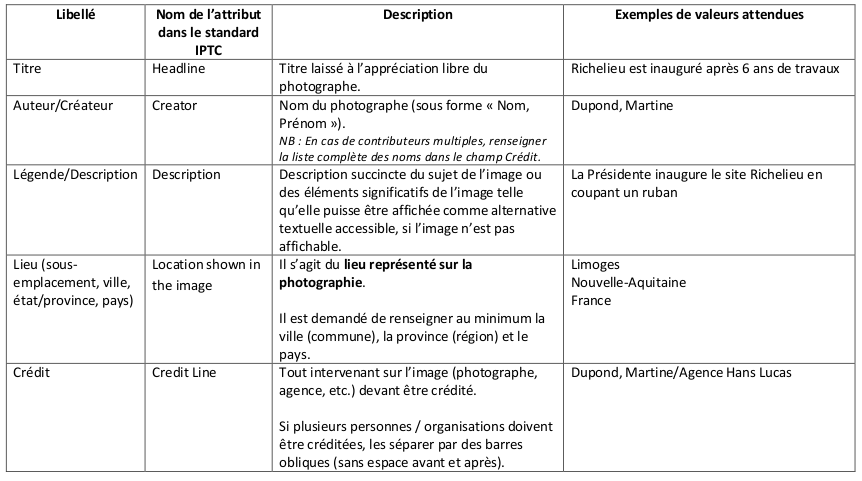
\includegraphics{./img/spe_iptc_bnf.png}
\end{adjustbox}
\caption{Liste des métadonnées IPTC obligatoires, Source : BnF, Spécifications des photographies nativement numériques}
\end{figure}

\begin{figure}[h]
	\begin{adjustbox}{width = \textwidth, center}
		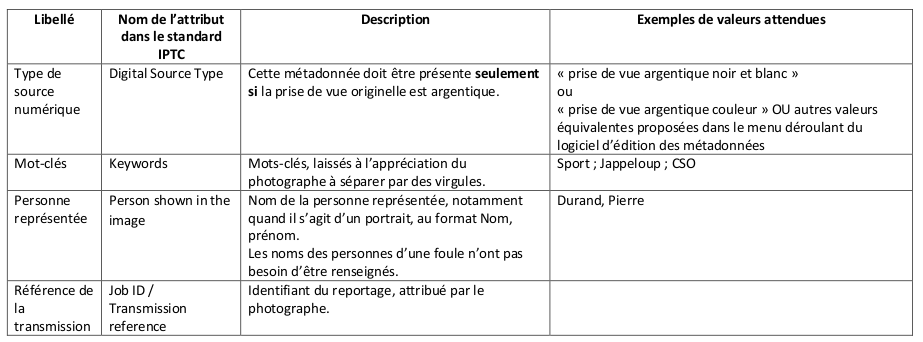
\includegraphics{./img/opt_iptc_bnf.png}
	\end{adjustbox}
	\caption{Liste des métadonnées IPTC optionnelles, Source : BnF, Spécifications des photographies nativement numériques}
\end{figure}
\newpage



\subsection*{Des exigences peu respectées}

Cependant, à l'issue de la collecte de l'ensemble des reportages, il s'est avéré qu'environ un tiers des photojournalistes n'ont pas respecté les spécifications, tant pour les métadonnées internes que pour les formats de fichier. Ainsi, plusieurs photographes ont envoyé des images au format TIFF 48 bits au lieu de 24 bits. De plus, beaucoup de champs de métadonnées n'ont pas été remplis, ou l'ont été sans suivre les recommandations de la BnF. 

Pour analyser les métadonnées renseignées, les équipes de la BnF se sont dotées du logiciel de visualisation d'images XnView, également utilisé aux Archives nationales, et qui permet d'afficher le contenu visuel ainsi qu'un éventail très large des métadonnées internes. Cependant, ce mode de visualisation ne permet pas d'afficher les métadonnées d'un ensemble d'images. Au cours de notre échange avec Alix Bruys, celle-ci nous expliquait que l'équipe en charge du traitement des photographies numériques avait engagé des réflexions pour mettre en place une méthode d'analyse plus systématique et plus massive des métadonnées internes à l'aide de l'application Exiftool\footnote{Voir le site de l'application : \url{https://exiftool.org/}}. Il s'agit de l'une des applications les plus performantes pour la lecture, l'écriture et l'édition des métadonnées internes d'images numériques, c'était donc également sur elle que s'était porté notre choix pour l'analyse des reportages photographiques de la Présidence de la République. Nous reviendrons sur le fonctionnement de cette application plus en détail dans le sixième chapitre de ce mémoire. 

Une différence notable avec le traitement des reportages photographiques de la Présidence de la République aux Archives nationales réside dans l'usage prévu des métadonnées internes : dans le cas de la BnF, celles-ci ne sont pas destinées au signalement, mais sont uniquement envisagées pour de futures études sur le fonds. Dans le processus d’acquisition de la BnF, la création des notices se fait manuellement, sans processus d'exploitation automatisée des métadonnées internes. Celles-ci étant plutôt destinées à des exploitations ultérieures dans un contexte de recherche scientifique, il n'a pas été demandé aux photojournalistes d'amender les fichiers qui ne respectaient pas les spécifications : l'ensemble des reportages a été accepté tel que versé. Le travail de description et d'indexation requis est conséquent, et dépend grandement de celui réalisé en amont par le photojournaliste. Cependant, il est sans commune mesure avec le travail de description requis pour les reportages de la Présidence de la République : s'il est long et laborieux de procéder au signalement des 200 reportages du projet \enquote{Radioscopie de la France : regards sur un pays traversé par la crise sanitaire}, il l'est d'autant plus pour les près de 8000 reportages de la Présidence de la République, réalisés entre la seconde mandature de Jacques Chirac et celle de François Hollande.
\\

Pour comprendre les écarts constatés entre les spécifications définies par la BnF et les résultats obtenus, plusieurs facteurs peuvent être évoqués. Il est possible que certains photographes n’aient pas disposé des outils nécessaires pour transformer leurs fichiers dans le format requis ou que les appareils utilisés n'aient pas permis produire directement le format attendu. Les photographes ont pu utiliser des applications qui ne prenaient pas en charge les champs de métadonnées spécifiés, ou n’étaient peut-être pas familiers avec les différents schémas de métadonnées (EXIF, XMP, IPTC). Par ailleurs, il est envisageable que certains photojournalistes aient pensé qu'envoyer des fichiers dans une qualité supérieure serait préférable, sans avoir conscience des contraintes spécifiques imposées par la diffusion sur Gallica, ni de l’impact sur l’espace de stockage. Si les raisons d'être des spécifications techniques n’ont pas été explicitement communiquées, les photographes ont pu ne pas en comprendre l'importance.

Ces interrogations mettent en lumière un problème similaire à celui rencontré lors du traitement des reportages de la Présidence de la République. Lorsque les photographes ou producteurs se concentrent uniquement sur une description ou une indexation qui répond à leurs besoins immédiats, sans avoir une connaissance ou une compréhension claire des besoins des futurs utilisateurs, ils peuvent ne pas les prendre en compte. Cette étude de cas a démontré que, même lorsque ces besoins sont clairement exprimés en amont, comme dans le cas de la BnF, cela ne garantit pas que les photographes respecteront scrupuleusement les consignes. Nous ne pouvons bien sûr pas exclure l'hypothèse d'une simple négligence, dans la mesure où ces descriptions n'impactent en rien le travail du photographe. De plus, le niveau de technicité exigé par les processus de migration de format ou de renseignement des métadonnées internes peut ne pas être acquis par certains photographes.

De manière plus générale encore, ces exemples nous poussent à nous interroger sur l'implication des services producteurs dans le processus archivistique. Si les besoins liés à une gestion pérenne des documents numériques étaient pris en compte dès leur production, bien des obstacles rencontrés lors de la reprise des reportages photographiques auraient pu être évités. Cela nécessiterait cependant une évolution des politiques de gestion documentaire à l'échelle des institutions, qui devraient alors implémenter les principes d'interopérabilité des données produites. Tant que ce ne sera pas le cas, nous ne pouvons attendre des services producteurs qu'ils se conforment à des exigences extérieures à leurs propres besoins. Il convient alors de s'adapter aux contraintes propres aux documents versés en cherchant, lorsque cela est possible, des solutions palliatives. L'utilisation des descriptions réalisées par la cellule photographique n'est pas pour autant inadaptée au signalement dans un contexte archivistique. Toutefois, il est important de rappeler qu'il s'agit d'une solution imparfaite, une béquille destinée à pallier les lacunes induites par les contraintes spécifiques à la reprise des reportages photographiques de la Présidence : notamment le manque de temps et de ressources humaines. Cette approche revient à fusionner l'objet numérique et sa description, les métadonnées internes faisant partie intégrante des informations embarquées dans l'archive photographique.



\chapter{La reprise des données pour un versement dans le nouveau système d'archivage électronique des Archives nationales}

Pour conclure le chapitre précédent, nous avons exploré les problématiques liées à l’indexation, en mettant en lumière les divergences entre les intérêts métier, les pratiques d’utilisation et les contraintes rencontrées dans le traitement des reportages photographiques de la Présidence de la République. Nous avons vu comment celles-ci se traduisent en défis concrets pour la manipulation des archives, notamment en raison des différences de pratiques et des contextes de production. Dans ce chapitre, nous allons approfondir ces questions en examinant comment elles s'articulent avec le projet de reprise des données en vue de leur versement dans le nouveau système d'archivage électronique (SAE) Vitam des Archives nationales. En effet, une connaissance de ce contexte normatif et institutionnel est indispensable pour comprendre ce qu'il permet en termes d'indexation et d'exploitation des métadonnées internes. De plus, cela nous permettra d'approfondir notre compréhension du fonds des reportages photographiques, dans la mesure où son traitement actuel ne peut être décorrélé des traitements antérieurs menés par les Archives nationales.

Pour cela, nous nous attacherons à présenter le cadre normatif et l'environnement dans lequel s’effectuent les versements des archives numériques, ce qui nous permettra de mieux comprendre les enjeux techniques propres aux Archives nationales. Cette analyse inclura une présentation des normes encadrant l'archivage électronique, ainsi qu'un examen du SAE des Archives nationales et de la manière dont le chantier de reprise des données s’inscrit dans ce contexte institutionnel et technique. Il s'agit ici de définir les contraintes spécifiques qui impactent la gestion et la préservation des archives numériques aux Archives nationales, et de comprendre comment les reportages photographiques de la Présidence s'intègrent dans ce cadre complexe.

\section{Le cadre de l’archivage électronique}

Dans cette section, nous allons examiner le cadre normatif et les principes fondamentaux de l'archivage électronique, ce qui nous permettra de mieux comprendre les contraintes et les spécificités associées à la gestion des archives numériques. Nous commencerons par définir ce qu'est un système d'archivage électronique (SAE), en nous appuyant sur les normes et les exigences qui le régissent. Ensuite, nous présenterons les modèles conceptuels clés, notamment l'Open Archival Information System (OAIS) et le Standard d'Échange de Données pour l'Archivage (SEDA). Sur ces bases, nous pourrons mieux saisir comment ces cadres influencent la gestion, la conservation et l'accès aux documents numériques aux Archives nationales.

\subsection*{Le système d'archivage électronique : une brique dans le système d'information archivistique}

Le Système d’Archivage Électronique (SAE) est une sous-composante spécialisée du Système d’Information (SI), conçue spécifiquement pour gérer les archives numériques. Un Système d’Information (SI) est un ensemble de ressources permettant de collecter, stocker, traiter et diffuser de l’information, structuré selon les besoins de l’institution qui l’utilise. Dans le cadre des services d’archives, ce SI est désigné par le terme Système d’Information Archivistique (SIA). Le SIA constitue l’infrastructure générale pour la gestion des archives, englobant les outils et procédures nécessaires à la gestion des documents, qu'ils soient physiques ou numériques. Il est souvent composé de plusieurs briques fonctionnelles, dont la brique de base est le logiciel-métier permettant la gestion des archives. Ce socle doit garantir la collecte, le classement, la conservation et la communication des documents\footcite{bothSystemeInformationArchivistique2020}.

Lorsque les services d’archives traitent des masses importantes de documents numériques, l'intégration d'un SAE au sein du SIA devient indispensable. Le SAE doit répondre aux exigences spécifiques définies par la norme NF Z 42-013, publiée par l'AFNOR en 1999 et révisée en 2000 puis en 2009. Cette norme établit les exigences et recommandations fonctionnelles, organisationnelles et d’infrastructure nécessaires pour la conception et l’exploitation d’un SAE. Contrairement aux systèmes de gestion électronique de documents (GED), les SAE sont adaptés aux exigences particulières de la gestion des documents d’archives. Ils doivent garantir la disponibilité, l’intégrité, la confidentialité des documents ainsi que la traçabilité des opérations. Conformément à cette norme, le SAE doit également gérer les éléments de preuve associés aux documents archivés, incluant la production et l’archivage de journaux quotidiens horodatés, qui intègrent des éléments de preuve tels que les empreintes uniques des fichiers, les dates et heures des opérations réalisées.

Pour assurer la gestion des archives électroniques, le SAE doit inclure des fonctionnalités de collecte, de conservation et de communication des documents numériques. Pour assurer une intégration efficace, des mécanismes doivent être établis pour permettre aux applications du SIA de déposer des documents électroniques dans le SAE ou de consulter ceux déjà versés. Cela implique la mise en place d'une interface et de protocoles de communication entre les deux systèmes\footcite{wakimSAESystemesStockage2011}. Plutôt que de conservation, dans le cas des documents numériques, on préfère le terme de pérennisation. Contrairement aux documents physiques qui nécessitent une conservation matérielle, les données numériques ne se détériorent en soi, mais peuvent subir des pertes brutales et irréversibles en cas de dégradation des supports. Des opérations de vérification des empreintes numériques permettent de garantir l'intégrité des fichiers et de détecter toute altération survenue lors des opérations de gestion au sein du SAE. Le SAE doit également gérer la conservation de copies, qui, dans le contexte numérique, ont valeur d'original\footnote{Voir chapitre \ref{sec:chap3} pour la définition de la notion d'original dans le contexte de la photographie nativement numérique}. La communication passe par la gestion des accès aux documents numériques. On distingue trois types de communication : publique (les lecteurs en salle), interne (le personnel des Archives) ou administrative à l’extérieur, lorsqu’un service demande communication d’un de ses dossiers déjà versé. Dans le contexte des Archives nationales, sur lequel nous reviendrons dans le prochain chapitre, le SAE permet la consultation par les archivistes et services versants par un système de cloisonnement, réservant l'accès aux archives aux utilisateurs autorisés. Les demandes de consultation du public sont gérées par une autre brique du SIA des Archives nationales.
\\

Les processus de versement, de conservation, de communication, de restitution et d’élimination des documents doivent être conformes aux principes définis par la norme OAIS (ISO 14721).

\subsection*{Présentation de la norme OAIS}

Le modèle de référence OAIS (Open Archival Information System), élaboré par le Consultative Committee for Space Data Systems en 2002 et standardisé par l'ISO en 2012, constitue un cadre conceptuel pour la gestion, l'archivage et la préservation à long terme des documents numériques. Il définit les concepts et éléments de base offrant une vue globale et cohérente de l'archivage numérique. En s'appuyant sur le formalisme UML (\gls{uml}), l'OAIS propose un modèle, indépendant de toute application particulière. L'architecture qu'il dessine est destinée à garantir l'accessibilité et l'intelligibilité des informations archivées au fil du temps.

Le modèle définit quatre principaux acteurs impliqués dans le processus d'archivage\footcite[pp.41-44]{banat-bergerArchivageNumeriqueLong2009}: 

\begin{enumerate}
\item L'archive, définie comme \enquote{une organisation chargée de conserver l'information pour permettre à une communauté d'utilisateurs cible d'y accéder et de l'utiliser}.
\item Le producteur, qui fournit l'information à conserver. Il n'est pas nécessairement le producteur de l'information et est plutôt associé à la notion de \emph{service versant} dans le contexte archivistique.
\item L'utilisateur, désigne ici une personne ou un système entrant en relation avec \emph{l'archive} pour rechercher et consulter l'information conservée.
\item Le management, qui représente les décideurs chargés de déterminer le mandat, les priorités et les orientations de l'archive, en cohérence avec la politique de l'institution. Souvent à l'origine des sources de financement, il peut donc décider de l'orientation des ressources et évaluer les performances de \emph{l'archive}.
  \end{enumerate}


Ces acteurs s'échangent de l'information sous la forme de paquets d’information, contenant les objets à archiver et les métadonnées nécessaires à leur visualisation et pérennisation. Nous avons présenté dans le chapitre 2 la forme des fichiers numériques, constitués d'une suite de 0 et de 1. Dans le modèle OAIS, ce fichier numérique est modélisé par l'objet \emph{contenu d'information}, constitué d'un \emph{objet données} qui ne peut être interprété qu'à l'aide \emph{d'informations de représentation}. Parmi ces informations de représentation, les \emph{informations de structure} permettent d'interpréter les séquences de bits et de les traduire en caractères ou, dans le cas des images numériques, en pixels ; tandis que les \emph{informations sémantiques} fournissent des éléments permettant de comprendre la signification des données, par exemple l'unité de mesure dans laquelle des données chiffrées seraient exprimées\footcite[p.45]{banat-bergerArchivageNumeriqueLong2009}. Ainsi, les informations de représentation doivent permettre de représenter et de comprendre le contenu d'information. Les informations de pérennisation quant à elles permettent à l'archive d'assurer ses responsabilités. Elles contiennent des informations de contexte, de provenance, d'identification (association d'un identifiant à chaque objet numérique) et d'intégrité (l'empreinte numérique du fichier)\footcite[pp.48-49]{banat-bergerArchivageNumeriqueLong2009}. 

Enfin, les informations de description correspondent aux métadonnées descriptives des archives, obtenues à partir d'une analyse des objet numériques et de leurs informations de représentation et de pérennisation. Elles ne font pas partie du contenu d'information, mais permettent aux utilisateurs de rechercher les données au sein du système d'archivage électronique\footcite[p.172]{rietschDematerialisationArchivageElectronique2006}. Les informations d’empaquetage  (Packaging  Information) permettent de mettre  en  relation  les  différents composants du paquet d'information, c'est-à-dire l'objet données et les informations associées.

L’OAIS spécifie trois types de paquets d'information : le SIP (Submission Information Package), fourni par le producteur et remis au service d'archives ; le AIP (Archival Information Package), qui est conservé au sein du SAE ; et le DIP (Dissemination Information Package), qui est mis à disposition des utilisateurs pour consultation. Le modèle décrit également les interactions entre ces acteurs, incluant le versement des objets numériques par les producteurs, leur stockage à long terme sous forme d’AIP par le service d'archives, et la fourniture des documents aux utilisateurs sous forme de DIP. Les systèmes d'archivage électronique (SAE), comme Vitam, illustrent l'application des principes du modèle OAIS. 

\subsection*{Le SEDA}
Le Standard d'échange de données pour l'archivage (SEDA) est le fruit d'une collaboration initiée en 2006 entre les Archives de France et l'ancienne direction générale de la modernisation de l'État (DGME), dans le cadre du programme ADELE (Action pour le Développement de l'Administration Électronique). L'objectif du SEDA est de faciliter l'interopérabilité entre le système d'information d'un service d'archives et les systèmes d'information de ses partenaires, comme les services producteurs et versants, lors de l'échange de données. Le SEDA repose sur des normes et standards préexistants, avec comme structure de base la norme ISO 14 721, aussi connue sous le nom de modèle OAIS (Open Archival Information System). Le langage \gls{xml} a été retenu pour structurer les informations dans ce standard. Le SEDA identifie cinq acteurs principaux susceptibles d'intervenir dans ces échanges : le service versant (TransferringAgency), le service producteur (OriginatingAgency), le service d'archives (ArchivalAgency), le service de contrôle (ControlAuthority), qui peut intervenir pour valider les transactions ; et enfin, le demandeur d'archives (Requester), qui peut être toute personne physique ou morale souhaitant consulter les archives conservées\footcite{sibilleStandardEchangeDonnees2015}.

Ce standard permet l'échange de paquets d'information, tels que définis dans le modèle OAIS, en distinguant l'archive, qui regroupe le contenu des données, les informations de représentation et les informations de pérennisation. Selon le SEDA, un paquet d'informations à verser (SIP) est constitué d'un bordereau de transfert et d'un ou plusieurs objets à archiver. Ce bordereau se trouve à la racine du SIP et décrit l'ensemble des métadonnées du paquet, comprenant un en-tête, une déclaration des objets binaires, une description des archives représentées par ces objets, des métadonnées descriptives et de gestion, et les identifiants du service versant et du service d'archives\footcite[p.14]{programmevitamStructurationSubmissionInformation2023}. La description du contenu (ContentDescription) permet de décrire l’Archive et ses subdivisions intellectuelles en lui associant des informations de description et d’indexation\footcite{sibilleStandardEchangeDonnees2015}.
\\

Bien que le SEDA détaille les processus de transfert de données numériques, il ne spécifie pas les règles de constitution des paquets à transférer. La structure du paquet et du bordereau dépend donc en grande partie du système d'archivage électronique utilisé. Lors de la conception du pipeline de données destiné à la reprise des reportages photographiques, nous nous sommes référés non seulement au dictionnaire du SEDA\footcite{siafseda}, mais nous avons également dû adapter l'outil aux exigences du SAE des Archives nationales. 


\section{L'archivage électronique aux Archives nationales : des années 1980 à nos jours}

Après avoir exploré le cadre normatif qui régit l'archivage numérique en France, il est essentiel de contextualiser ces principes au sein des Archives nationales. Cette section explore le contexte spécifique de l'institution, en retraçant l’évolution de l’archivage électronique depuis les premières initiatives avec le programme Constance jusqu’à l’adoption du système d’archivage électronique Vitam. À travers cette analyse, il s’agit de comprendre comment ces évolutions institutionnelles et technologiques ont influencé le cadre de mon stage, qui a abouti à la conception d’un pipeline de données pour la reprise des reportages photographiques de la Présidence de la République en vue d'un versement dans le SAE Vitam. Ce parcours permet également de comprendre les traitements appliqués aux fonds archivés avant l'ère Vitam, mais aussi de poser les bases de notre réflexion sur la manière dont les paquets d'archives doivent être construits pour répondre aux exigences de ce nouveau système d'archivage.

\subsection*{L'aube de l'archivage électronique aux Archives nationales : le programme Constance}

Les Archives nationales de France ont entrepris la collecte d’archives numériques dès 1982 grâce au programme Constance (CONServation et Traitement des Archives Nouvelles Constituées par l’Électronique), un projet pionnier qui a défini la politique, les processus, et les méthodes de traitement et de conservation des données numériques et de leurs métadonnées. Par extension, le service chargé de l’archivage électronique au Centre des Archives Contemporaines (CAC) du site de Fontainebleau a aussi été surnommé \emph{Constance}. Pendant plus de 30 ans, Constance a permis de collecter et de préserver les données issues d'enquêtes statistiques, avec des processus tels que la gestion des fichiers et de leurs métadonnées dans une base documentaire et leur archivage sur des bandes magnétiques \gls{lto}, en planifiant régulièrement des migrations de support. Des conversions de fichiers ont également été opérées dans une optique de conservation des documents bureautiques, notamment la conversion de fichiers Word au format PDF alors réputé plus pérenne \footcite{levasseurRetourExperienceStrategie2022}. 

Pour parer aux risques d'obsolescence technologique, l'équipe de Constance a adopté des solutions visant à assurer la pérennité des fichiers numériques, \enquote{quelle que soit leur forme technique}\footcite[p.62]{conchonArchivageFichiersInformatiques1988}, bien que les mutations technologiques incessantes mettent à mal cette noble tentative. Les données sont stockées sur des bandes LTO, un support plus durable et offrant de plus grandes capacités que les disques optiques. Néanmoins, les CD et DVD, apparus après les bandes LTO, ont été recommandés pendant les années 2010 pour la conservation à des fins d'archivage. Cependant, les migrations régulières vers de nouveaux supports demeurent inévitables : il n'existe pas à ce jour de support qui ne se dégrade pas au fil du temps. A titre d'exemple, les bandes LTO sont réputées fiables sur une période de 15 à 30 ans, bien que des migrations à des échéances plus courtes soient nécessaires afin de minimiser les risques de pertes de données\footcite{verlhiacQuEstceQue2023}. La durée de vie des CD et DVD dépasse rarement 10 ans, tandis que celle des disques durs externes de type HDD est estimée entre 5 et 7 ans. Sur ces bandes LTO, les fichiers sont conservés \enquote{à plat}, c'est-à-dire sans structure ou classement issus de logiciels métier ou d'une arborescence antérieure de dossiers et de sous-dossiers. 

Le programme Constance a également mis en place un système de nommage des fichiers, qui inclut plusieurs métadonnées, telles que le numéro de notice du producteur, le numéro d'entrée, le numéro d'article, le nom du fichier d'origine, et son extension, afin de faciliter leur identification et leur traçabilité dans le temps. Voici, par exemple, le nommage d'un fichier issu des reportages photographiques traités sous la mandature de Jacques Chirac : 

\begin{displayquote}
	\begin{center}
		009918\_20100562\_3546\_35460001.JPG
	\end{center}


Il s'agit ici d'un fichier au format JPEG, la première photographie du reportage 3546 (nom du fichier d'origine), dans le dossier correspondant au reportage 3546 (numéro d'article), de l'entrée 20100562, versé par le service photographique de la Présidence de la République, dont le numéro de notice producteur est 009918 (FRAN\_NP\_009918).
\end{displayquote}

Le programme Constance a évolué, passant de la conservation de données structurées issues d'applications informatiques, principalement des statistiques, à la prise en charge de nouveaux types de documents numériques, tels que les fichiers bureautiques, les messageries, les images, les vidéos et les documents sonores. Ce changement a été particulièrement marqué après 2010, lorsque les archives nativement numériques provenant des administrations centrales ont commencé à dominer les versements, rendant obsolètes certaines pratiques du programme initial\footcite{sinblimabarruArchivageNumeriqueAux2015}. En réponse à ces évolutions, le service Constance s'est réorganisé en 2012 au sein du Département de l'archivage électronique et des archives audiovisuelles (DAEAA) des Archives nationales, pour mieux gérer la diversité croissante des formats et des types de données.

Le projet ADAMANT (Administration des Archives et de leurs Métadonnées aux Archives Nationales, dans le Temps), lancé en 2015, a été conçu pour faire évoluer les pratiques d'archivage électronique aux Archives nationales, en réponse à l'inadéquation croissante du programme Constance face aux enjeux de l'archivage numérique des années 2010\footcite[p.220]{marcotteArchivesConduiteChangement2015}. En particulier, Constance ne permettait plus de gérer efficacement l'intégration des fonds physiques et numériques, une exigence devenue centrale avec l'augmentation des archives nativement numériques. ADAMANT s'inscrit ainsi comme un projet organisationnel et d'accompagnement au changement, visant à ne plus séparer la responsabilité des fonds en fonction de leur support. Ce projet a conduit à l'ouverture du SAE des Archives nationales en 2018 et à la création du Département de l'administration des données (DAD), qui a pris la suite du DAEAA.
\\

La méthode Constance est maintenue jusqu’à l’ouverture du système d'archivage électronique des Archives nationales en novembre 2018. Cependant, l'application des traitements étant un processus très chronophage, avec le renommage des fichiers et leur mise à plat, l'ensemble des archives versées avant 2018 n'a pas pu être traité intégralement. C'est notamment le cas des reportages photographiques de la Présidence de la République et des Services du Premier ministre, dont seulement une partie a été traitée. Après la décision de passer au système d'archivage électronique Vitam, il n'était plus nécessaire -- voire contre-productif -- de continuer l'application de la méthode sur les documents versés.

\subsection*{Le SAE Vitam}

Le programme Vitam (Valeurs immatérielles transmises aux archives pour mémoire), lancé officiellement le 9 mars 2015, est un projet interministériel d’archivage électronique conçu pour répondre aux défis contemporains de la gestion massive de documents numériques. Développé par trois ministères (Affaires étrangères, Culture, Armées) sous la supervision du Comité interministériel aux Archives de France et de la Direction interministérielle du Numérique, Vitam vise à proposer une solution logicielle libre, capable de traiter de larges volumes de documents nativement numériques de tout type (bureautiques, audiovisuels, bases de données). La solution logicielle doit garantir l'intégrité et la pérennité (respect de la valeur probante) des documents numériques, leur sécurité (duplication des serveurs, cybersécurité, souveraineté des espaces de stockage) et leur facilité d’accès pour un usage fréquent. 

Déployé progressivement entre 2015 et 2023 au sein des ministères porteurs à travers des plateformes adaptées comme \emph{Saphir} pour le ministère des Affaires étrangères, \emph{Archipel} pour le ministère des Armées et \emph{Adamant} pour les Archives nationales, Vitam se concentrait initialement sur des applications de backoffice. La conception des interfaces utilisateur était laissée à la charge de chaque institution, selon ses besoins spécifiques. Le programme Vitam s’inscrit dans une démarche collaborative, avec une communauté d’utilisateurs actifs qui a contribué à son évolution. Cette approche a mené à l’élaboration de Vitam UI, dont le développement a débuté en 2019, pour répondre aux besoins de nouveaux utilisateurs n'ayant pas les moyens de créer leur propre interface. L’ensemble des exigences fonctionnelles découlant du cadre normatif évoqué dans le chapitre précédent a orienté le fonctionnement et l’architecture de Vitam : la norme NF Z 45-013 pour le système d’archivage électronique (SAE), la norme OAIS pour les interactions et la traçabilité, et le format SEDA pour la modélisation de l'ensemble des transactions définies par la norme OAIS.

Conformément au modèle conceptuel OAIS, la solution logicielle Vitam prend en entrée des paquets d’informations (Submission Information Packages, ou SIP). Or, cette dernière ne permet pas de générer les SIP à partir des fichiers et de leurs métadonnées. Cette fonction est déléguée à un outil tiers, appelé ReSIP, intégré dans un second temps à l'architecture Vitam et téléchargeable sur le site officiel de la solution logicielle. Une fois le SIP constitué à l’aide de l’outil ReSIP, il se présente sous la forme d’un conteneur (.zip ou .tar) comprenant un répertoire contenant l’ensemble des objets numériques mis à plat, ainsi qu’un bordereau, communément appelé le \emph{manifest}. Ce document contient l’ensemble des métadonnées descriptives
et informations de pérennisation décrites dans le chapitre précédent : il permet notamment de reconstituer l’arborescence des objets numériques après leur ingestion dans Vitam et d’attribuer une empreinte unique à chaque
objet.
\\

Comme évoqué dans l'introduction de ce mémoire, l'application conçue au cours de mon stage au Département de l'administration des données (DAD) s'inspire des fonctionnalités de ReSIP (mise à plat des fichiers, écriture du manifest) en s'adaptant aux besoins spécifiques de la reprise des reportages photographiques par l'ajout d'une étape d'extraction des métadonnées internes des fichiers afin d'enrichir le signalement des versements dans le SIA des Archives nationales. Il est important de préciser cependant qu'à ce jour, le SIA des Archives nationales ne permet pas la recherche par mots-clés : s'ils apparaissent bien dans l'interface, ils ne peuvent être recherchés par le moteur de recherche ou à l'aide de filtres à facettes. Seuls quelques champs sont interrogeables, notamment le titre de l'unité d'archive et sa cote. Cette limitation ne vient pas du SAE Vitam mais bien de l'interface des Archives nationales qui ne rend pas interrogeable l'ensemble des métadonnées descriptives du paquet. Cette spécificité découle d'un choix effectué au moment de la conception de cette partie du SIA,, choix qui pourrait être révisé pour améliorer l'interrogabilité des fonds. Cette possibilité nous a conforté dans notre décision d'exploiter les métadonnées internes des photographies dans l'hypothèse où une mise à jour du SIA permettra à terme d'étendre les champs interrogés par le moteur de recherche.

\section{Le chantier de reprise des données des reportages photographiques de la Présidence et des services du Premier ministre}

Le travail produit dans le cadre de mon stage s'inscrit dans le contexte plus global du chantier de reprise des données conservées sur disques-durs et sur bandes LTO vers le nouveau système d'archivage électronique Vitam des Archives nationales. Après une présentation de la reprise des données, nous nous intéresserons aux spécificités des fonds de reportages photographiques qui ont nécessité l'élaboration de plusieurs méthodes de traitement. La méthode de reprise semi-automatique des reportages des services du Premier Ministre sera ensuite présentée : elle correspond à un premier état des réflexions qui ont mené, dans un second temps, à la conception du pipeline de données qui automatise le traitement d'une partie des reportages photographiques de la Présidence de la République.

\subsection*{Présentation du projet}

Le passage de la méthode Constance au SAE Vitam entraîne non seulement un changement de méthode, mais aussi une évolution du support de stockage des archives numériques. Les archives numériques versées avant la mise en place du SAE sont stockées sur des bandes LTO ou sur des disques durs pour les dernières entrées non traitées. Cet état de fait n'est satisfaisant ni sur le plan de la communication ni sur celui de la sécurisation, les archives n'étant pas accessibles aux divers utilisateurs et les supports matériels se dégradant au fil du temps. Le chantier de reprise des données a donc pour objectif de transférer l'ensemble des documents versés avant la mise en place du SAE Vitam vers cette nouvelle plateforme d'archivage électronique. Les reportages photographiques concernant les mandatures de Jacques Chirac, Nicolas Sarkozy et François Hollande ayant été versés avant cette migration, ils font partie de cet ensemble à reprendre.

Le chantier de reprise des données mis en place en 2019 par Martine Sin Blima-Barru, responsable du DAD, a été confié à Émeline Levasseur\footnote{La description du chantier de reprise des données développée dans cette partie s'appuie sur des documents de communication internes produits au sein du service : \enquote{Retour AMOA reprise des données structurées}, présentation PowerPoint du 7 octobre 2019, et \enquote{La reprise des données et des métadonnées formant le patrimoine numérique des Archives nationales}, présentation PowerPoint du 18 mars 2021.}. La première étape du processus de reprise a consisté en l'analyse des données transférées sur serveurs après avoir été extraites des bandes LTO ou des disques durs. Pour rendre accessibles leurs métadonnées, la cartographie des fonds à reprendre devait permettre de lister les sources d'informations et de les associer aux archives correspondantes : exports CSV des bases de données Cindoc, instruments de recherche publiés ou non, etc. L'association entre ces métadonnées externes et les fichiers nécessitait l'identification de valeurs pivots telles que le numéro de versement ou le numéro d'article. Les métadonnées disponibles ont été divisées en plusieurs catégories en fonction de leur utilité : métadonnées descriptives, métadonnées techniques, métadonnées de gestion. Cette étape de cartographie a également permis de distinguer les métadonnées disponibles de celles qui restaient à déterminer (nombre de fichiers, poids, formats des données).

La cartographie des données et des métadonnées a permis leur catégorisation en différentes typologies homogènes : bureautique, photo-audiovisuel, données structurées, messageries, archives orales. L'intérêt de cette catégorisation étant d'envisager des méthodologies de traitement similaires pour chaque ensemble homogène. A l'identification de ces grands ensemble s'ajoutent des préoccupations archivistiques qui ont permis de déterminer des priorités quant à l'ordre des reprises : le besoin de rendre accessibles les fonds communicables, la nécessité d'avoir repris les versements auxquels s'ajouteront de nouvelles entrées, la prise en compte de l'espace occupé sur les serveurs.

A l'intérieur de chacun des ces grands ensembles, il peut ensuite être nécessaire d'établir une catégorisation plus fine afin de déterminer si une seule méthode de reprise peut être appliquée à l'ensemble des données, ou s'il sera nécessaire d'adapter la méthode à des spécificités propres à chaque versement. Au cours de mon stage de première année de master en 2023, j'ai effectué une première analyse des fonds de reportages photographiques de la Présidence de la République et des services du Premier ministre dans cette perspective. Cette première analyse, confortée lors de mon stage de master 2 en 2024, a révélé l'hétérogénéité de ces reportages. Il convenait alors de développer des méthodes spécifiques à chaque service producteur, mais également au sein même des versements.


\subsection*{Hétérogénéité des fonds}

Les évolutions des pratiques d’archivage électronique aux Archives nationales ont engendré une hétérogénéité notable dans le classement des fonds de reportages photographiques. Les reportages traités selon la méthode Constance, caractérisée par le renommage systématique des fichiers et leur mise à plat, contrastent avec ceux qui ont été partiellement ou non traités et qui présentent une organisation plus variée et moins uniforme. Dans ce contexte, il apparaît pertinent de différencier la reprise des reportages des services du Premier ministre de celle des reportages de la Présidence de la République. Les reportages du Premier ministre sont relativement homogènes, ayant été largement traités suivant la méthode Constance. De plus, leur volumétrie reste plus modeste et donc plus facilement appréhendable par rapport aux fonds des reportages de la Présidence. Cette homogénéité justifie l'adoption d'une méthode spécifique de fabrication des SIP et d’ingestion pour l’ensemble de ces reportages. Un enjeu central de ce processus réside dans la gestion de l’arborescence des dossiers : faut-il récupérer une arborescence existante ou reconstituer une arborescence perdue mais conservée intellectuellement dans le nommage des fichiers ? La réponse à cette question déterminera nécessairement des approches méthodologiques distinctes.

Pour les reportages de la Présidence, divers scénarios ont été identifiés, chacun présentant des caractéristiques distinctes :

\begin{enumerate}
\item Reportages de la mandature de Jacques Chirac non traités 1 : Un dossier par reportage, subdivisé en plusieurs sous-dossiers pour chaque séquence. Les fichiers, souvent non renommés, peuvent être organisés de manière complexe avec plusieurs niveaux de sous-dossiers, incluant à la fois des séquences et des sélections de photographies.
\item Reportages de la mandature de Jacques Chirac non traités 2 : Un dossier par reportage avec des fichiers non renommés à plat, accompagné d’un ou plusieurs dossiers de photographies sélectionnées.
\item Reportages de la mandature de Jacques Chirac traités : Un dossier par reportage avec les fichiers renommés à plat. Une arborescence disparue peut être reconstituée à partir des noms de fichiers.
\item Reportages de la mandature de Nicolas Sarkozy traités : Un dossier par mois avec les fichiers renommés à plat. Une arborescence disparue peut être reconstituée au sein d’un même reportage à partir des noms de fichiers.
\item Reportages de la mandature de Nicolas Sarkozy non traités : Un dossier par mois puis un dossier par reportage, avec plusieurs niveaux de sous-dossiers pour diviser les reportages en séquences. Les fichiers ne sont pas renommés.
\item Reportages de la mandature de François Hollande : Un dossier par année puis un dossier par reportage, avec plusieurs niveaux de sous-dossiers pour organiser les séquences des reportages. Les fichiers ne sont pas renommés.
\end{enumerate}

Lors de mon stage de Master 2, il a été décidé de développer une méthode spécifique, suivie par la création d’une application (ou pipeline de données) sur le fonds le plus homogène, à savoir celui de François Hollande. Cette application vise à restituer une arborescence déjà existante plutôt qu’à la recréer à partir du nommage des fichiers, répondant ainsi aux besoins particuliers de ce fonds. Cette application pourra être ensuite utilisée pour la reprise des autres reportages non traités, ou servir de base à une future méthode de traitement.

D’autres différences entre les fonds de la Présidence et du Premier ministre ont également mené à des solutions d’archivage distinctes, notamment en ce qui concerne la richesse et la qualité des métadonnées internes. Le fonds du Premier ministre, avec une indexation et une description moins détaillées, justifie une approche différente. Il a été jugé moins pertinent de conserver une indexation au niveau de chaque photographie, surtout vu le faible niveau de granularité des descriptions, qui sont souvent associées à des groupes de photographies plutôt qu’à des photographies individuelles. Cette réflexion a conduit à la décision de remonter le contenu des mots-clés au niveau des reportages, un travail de normalisation rendu plus envisageable par la moindre richesse des mots-clés et la plus petite taille de ce fonds par rapport à celui de la Présidence.
\\

Dans la partie suivante, je présenterai en détail le processus de reprise des reportages des services du Premier ministre. Ce processus, bien que semi-automatique, a été crucial pour alimenter les réflexions sur l’automatisation des traitements des reportages présidentiels. 

\subsection*{Une solution semi-automatique pour les reportages photographiques des services du Premier ministre}

Les reportages photographiques du service du Premier ministre sont regroupés dans des paquets d’archives, ou SIP, générés par le logiciel ReSip. Ce processus s’appuie sur une méthode d’importation de données reposant sur un fichier CSV de métadonnées. Chaque paquet correspond à une période de l’année, suivant une logique volumétrique et regroupe l’ensemble des données à verser ainsi que les métadonnées associées. Avant la constitution des paquets, une réorganisation des fichiers a été nécessaire. Le nommage des fichiers ayant suivi la méthode Constance, cette standardisation du nommage a permis, grâce à des commandes Powershell, de reconstituer une arborescence de dossiers correspondant aux différents reportages. Cette étape a facilité l’organisation des fichiers selon le classement adopté dans l’instrument de recherche.

La méthode de constitution des paquets est uniforme pour tous les reportages photographiques des services du Premier ministre, incluant le choix des métadonnées conservées ou créées lors de la reprise des données. Ce processus semi-automatisé repose sur la création de tableurs, sous forme de fichiers CSV de métadonnées, qui sont ensuite importés dans ReSip. Ce modèle de tableur peut être appliqué à l’ensemble des paquets à créer, garantissant ainsi une méthode reproductible et efficace. Pour constituer un paquet, il est nécessaire de préparer un CSV de métadonnées inventoriant les fichiers de données et leurs métadonnées descriptives. Ces CSV sont réalisés manuellement à partir de deux sources se présentant elles-mêmes sous la forme de tableurs : l’instrument de recherche et les métadonnées internes des photographies, extraites avec l’outil ExifTool. Seules certaines informations issues de ces sources sont migrées vers le système d’archivage électronique : les dates et intitulés des reportages ainsi que les anciennes cotes, provenant de l’instrument de recherche, et les dates et heures de prise de vue, noms des photographes, informations de localisation et mots-clés issus des métadonnées internes des photographies.

Les informations de localisation et les mots-clés, souvent associés à un ensemble de photographies ou à l’ensemble d’un reportage, sont reportés au niveau du reportage pour assurer une indexation plus pertinente et fiable. Les noms des photographes, lorsqu’ils sont disponibles, sont documentés au niveau de chaque photographie pour une meilleure traçabilité, notamment dans les cas où plusieurs photographes ont couvert le même reportage. Toutes ces informations sont ensuite nettoyées, soit directement dans Excel, soit dans \gls{openrefine}. Une fois les CSV de métadonnées constitués, ils sont importés dans ReSip, qui génère les SIP destinés à être transférés dans le SAE des Archives nationales. 

Pour faciliter l’application de cette méthode, j’ai rédigé un guide détaillé, disponible en annexe, qui présente pas à pas chaque étape du processus décrit ci-dessus\footnote{Voir le pas à pas en annexe \ref{sec:annexe2}.}.
\\

Dans ce chapitre nous avons présenté le cadre normatif et institutionnel de l'archivage électronique aux Archives nationales. Cette présentation a permis d'expliciter les règles auxquelles devra se conformer l'application de reprise des reportages photographiques de la Présidence, mais aussi les traitements antérieurs effectués sur les archives à reprendre. En effet, le chantier de reprise des archives numériques doit prendre en compte les traitements induits par la méthode Constance et les exigences de la nouvelle solution d'archivage Vitam. Si les reportages photographiques des services du Premier ministre, intégralement traités, ont pu être repris en suivant une seule et même méthode, ce n'est pas le cas des reportages de la Présidence de la République qui présentent plusieurs états de traitement. Nous avons présenté la méthode semi-automatique de reprise des reportages des services du Premier ministre, qui convenait à un fonds homogène et d'un volume relativement réduit. En revanche, l'hétérogénéité du classement des reportages de la Présidence, ainsi que sa volumétrie bien supérieure, ne sont pas compatibles avec une solution de reprise semi-automatique. Face à la masse des données, il devient nécessaire d'envisager des solution d'automatisation qui intègrent les apports qualitatifs d'un traitement manuel, notamment l'indexation au niveau des fichiers. 	
\chapter{Des solutions d'automatisation face à la masse des données}

Comme évoqué dans le chapitre précédent, l'augmentation exponentielle de la production documentaire impose la mise en place de solutions d'archivage capables de gérer efficacement cette masse croissante tout en maintenant un haut niveau de qualité dans le traitement des données. En effet, les fonds d'archives très volumineux posent un double défi : ils sont non seulement plus longs et complexes à décrire, mais leur manque de description approfondie peut les rendre inaccessibles. Sans une indexation efficace et des métadonnées descriptives interrogeables, ces fonds risquent de devenir inexploitables. Il est donc impératif de développer des stratégies pour maîtriser cette masse documentaire, notamment par l'élimination de fichiers quasi-identiques et par un signalement qui assure une indexation efficace. Ce chapitre propose d'explorer plusieurs solutions offertes par les technologies numériques pour automatiser le traitement archivistique dans ce contexte de production exponentielle. Nous commencerons par examiner les avantages et les inconvénients de l'intelligence artificielle, qui est devenue incontournable dans le paysage numérique actuel. Ensuite, nous nous pencherons sur des solutions moins coûteuses et plus accessibles, adaptées à des projets de petite à moyenne envergure. Enfin, nous aborderons les défis spécifiques liés à la volumétrie des reportages photographiques, en particulier dans le contexte des Archives nationales et du système d'archivage électronique Vitam, et les solutions sur mesure qui ont été adoptées pour surmonter ces obstacles.

\section{Avantages et inconvénients d’un recours à l’intelligence artificielle pour le traitement des archives iconographiques}

\subsection*{L'intérêt de l'intelligence artificielle pour l'indexation des archives iconographiques}

L’intelligence artificielle ouvre aujourd’hui la voie vers des solutions précieuses pour l’indexation des archives, notamment iconographiques, un domaine confronté à des défis liés à l’augmentation exponentielle de la production documentaire numérique. La capacité de l’IA à analyser et à traiter de grandes quantités d’images permet d'automatiser les processus d'indexation, rendant ainsi les archives plus accessibles et exploitables. Le \emph{deep learning}, une branche du \emph{machine learning}, est particulièrement pertinent dans ce contexte. Les algorithmes de \emph{deep learning}, inspirés par les réseaux de neurones du cerveau humain, sont capables de reconnaître des motifs complexes au sein des images\footcite[pp.3-4]{marcus2018deep}. Grâce à l'entraînement sur des ensembles de données volumineux et variés, ces algorithmes peuvent identifier et cataloguer les éléments visuels présents dans les photographies, comme des objets, des lieux, ou des personnes.

Le \emph{transfer learning}, qui permet d’adapter des modèles préexistants à de nouveaux ensembles de données sans ré-entraînement complet, confère une flexibilité supplémentaire à ces outils\footcite[pp.8-9]{marcus2018deep}. Cela signifie qu’une IA, entraînée initialement à reconnaître des motifs spécifiques, peut être réajustée pour répondre aux besoins d’un service d’archives, en se concentrant par exemple sur la reconnaissance de visages. Cette capacité d’analyse des images permet de générer automatiquement des mots-clés pertinents qui enrichissent les métadonnées associées aux fichiers, facilitant ainsi la recherche et l'interrogation des archives par les utilisateurs\footcite{langevinTechnologiesIntelligenceArtificielle2022}.

Si un algorithme est bien entraîné à reconnaître un humain, de nombreuses données d’entraînement demeurent nécessaires pour lui permettre de distinguer les individus et donc d’identifier précisément les personnes représentées : il faut lui avoir fourni en amont des données d’entraînement nombreuses sur chacune des personnes qu’on souhaite identifier. Un tel processus demande beaucoup de temps de préparation des données d’entraînement : il faut disposer de vues nombreuses et variées de toutes les personnes, lieux ou situations que l’on souhaite pouvoir identifier, et avoir procédé à cette indexation sur l’ensemble de ces données d’entraînement. De plus, ce travail de description nécessite en amont un autre travail de réflexion afin de déterminer les mots-clés que l’on souhaite faire remonter : comme nous l’évoquions au début de ce mémoire, le potentiel descriptif d’une photographie est presque illimité, il est donc difficile de déterminer au préalable l’ensemble des termes que l’on souhaite associer sans avoir dans un premier temps analysé le fonds dans son intégralité. Le \emph{clustering} permet une approche inverse qui ne repose pas sur une indexation préalable mais invite l’IA à proposer des regroupements de données en un nombre de catégories, prédéfini ou non, mais dont les critères de rassemblement sont déterminés par l’IA elle-même. Si cette solution semble plus adaptable, elle ne permet pas d’imposer un vocabulaire normé issu des réflexions des archivistes, et risque d’entraîner l’indexation de termes peu pertinents dans un contexte archivistique.

\subsection*{L'intérêt de l'IA pour identifier les photographies sensibles}

L’intelligence artificielle offre également de nouvelles possibilités dans la gestion des documents contenant des informations sensibles, qu'il s'agisse de données personnelles ou de contenus classifiés. L’enjeu est donc d’empêcher la communication de données sensibles, mais aussi de pouvoir librement communiquer les documents qui n’en contiendraient pas et dont les délais de communication sont repoussés en raison de l’incapacité des archivistes à analyser les fonds dans leur intégralité. Cette solution serait particulièrement intéressante dans le contexte des reportages photographiques de la Présidence dont le contenu potentiellement sensible impose le contrôle des fichiers demandés avant toute communication. 

L’IA peut jouer un rôle dans l’identification des photographies non communicables. Par exemple, les algorithmes de reconnaissance faciale peuvent être utilisés pour détecter et identifier les visages d'enfants, assurant ainsi le respect du droit à l'image des personnes mineures. De plus, elle peut être programmée pour analyser les titres ou les descriptions des reportages photographiques afin d’identifier des termes spécifiques, indiquant la présence de contenus sensibles protégés par le droit à l’image ou la législation sur la défense nationale. Dans ces cas, l’IA peut automatiquement assigner des règles de gestion spécifiques, telles que l’extension des délais de communicabilité ou l’obligation de flouter certaines parties des images avant leur diffusion\footcite{baronDarkArchivesEdemocracy2017}. Cette capacité à sécuriser et gérer automatiquement les archives sensibles non seulement protège les données mais assure également un meilleur respect des exigences légales et éthiques, tout en optimisant le processus de gestion documentaire.
Cependant, l'IA n'est pas infaillible et peut commettre des erreurs, notamment dans l'identification des visages ou l'attribution de mots-clés, ce qui peut avoir des conséquences significatives en matière de protection des données. Ainsi, un contrôle humain reste indispensable pour valider les résultats produits par les algorithmes et corriger les éventuelles anomalies.

\subsection*{Gérer la masse en identifiant les prises de vue quasi-identiques}
Il n’est pas question de procéder à des éliminations dans le contexte de la reprise des reportages photographiques aux Archives nationales. Les éliminations sont, le cas échéant, effectuées en amont par le service chargé de l’archivage intermédiaire. Cependant, d’un point de vue purement théorique, il peut être intéressant de s’interroger sur la pertinence de confier ce tri à une intelligence artificielle, les services versants n’ayant pas toujours les moyens de procéder à un tri efficace.

La gestion des prises de vue quasi-identiques, produites en rafale par des appareils numériques modernes, représente un défi majeur pour les archivistes chargés de fonds de photographies numériques. Ces séquences d'images, souvent très similaires, peuvent rapidement saturer les bases de données et rendre la gestion des archives plus complexe. L'intelligence artificielle offre une solution efficace à ce problème en identifiant et en regroupant ces images quasi-identiques. Grâce à des algorithmes spécialisés, l’IA peut analyser les variations minimes entre les prises de vue successives et les classer en groupes homogènes\footcite{rolan2019more}. Ce processus permet de réduire la redondance en sélectionnant automatiquement les images les plus représentatives de chaque séquence, tout en éliminant celles qui semblent redondantes. En conséquence, l'utilisation de l'IA permet d'alléger le volume des fichiers à traiter, de rationaliser l'organisation des archives et de faciliter l'accès aux documents les plus pertinents pour les utilisateurs. Cette gestion des images redondantes ne se limite pas à la réduction de la masse des archives, mais contribue également à l'optimisation des ressources de stockage.
La question subsiste toutefois des critères appliqués par l’algorithme pour sélectionner les clichés jugés les plus pertinents, une telle sélection pouvant être particulièrement subjective. Pour rendre un recours à l’IA adapté à ce contexte, il serait nécessaire d’ajouter une étape d’évaluation humaine des regroupements effectués.
\\

Malgré les promesses de l’IA dans le traitement des archives, il est essentiel de reconnaître les limites de ces technologies. Au-delà des limites évoquées précédemment, la mise au point et l’implémentation d’une IA dans un service nécessite des ressources humaines, financières et documentaires importantes pour le nettoyage et l’indexation des données d’entraînement, ainsi que pour garantir une puissance de calcul suffisante des machines locales. Par ailleurs, le jeu de données doit en valoir la chandelle : les données à traiter doivent être assez nombreuses pour que les données d’entraînement demeurent une minorité.

De plus, l'une des critiques majeures à l'encontre de l'IA concerne l'opacité de ses processus décisionnels, souvent qualifiés de \enquote{boîte noire}. L’absence de transparence dans le fonctionnement interne des algorithmes de \emph{deep learning} rend impossible la documentation des choix archivistiques, un aspect pourtant fondamental du métier d'archiviste. Cette opacité peut poser problème lorsqu’il s’agit de justifier les décisions prises par l’IA, notamment dans le cadre de l’évaluation et de la classification des documents. En conclusion, bien que l’IA offre des outils puissants pour améliorer le traitement des archives iconographiques, son intégration dans les pratiques archivistiques dépend des moyens du service, du délai de traitement permis, et de la volumétrie du fonds. Toutes ces limites excluent un recours à l’intelligence artificielle dans le contexte de la reprise des données des reportages photographiques de la Présidence de la République aux Archives nationales.

\section{Les possibilités actuelles de gestion de la masse aux Archives nationales}

Si une nouvelle évaluation ou un nouveau tri ne peuvent être réalisés, et que les moyens humains et le temps nécessaire pour décrire les photographies font défaut, le recours à l'intelligence artificielle devient également inenvisageable. Dans ce contexte, nous ne pouvons que nous tourner vers la solution initialement évoquée : exploiter les descriptions et indexations déjà produites par la cellule photographique. Il s'agit donc de tirer parti des ressources existantes, notamment en mettant en place des méthodes d'extraction en masse de ces métadonnées, en identifiant les doublons pour éviter l'archivage redondant, et en développant des solutions adaptées aux contraintes volumétriques imposées par le système d'archivage électronique Vitam.

\subsection*{Extraction et calcul de métadonnées en masse}

\subsubsection*{L'extraction de métadonnées techniques et descriptives avec Exiftool}

Il est relativement simple d'accéder aux métadonnées internes des images numériques. Certains visualiseurs d'images, comme XnView, permettent non seulement d'afficher le contenu graphique, mais également de consulter un large éventail de métadonnées associées aux fichiers. À défaut de disposer d'une application dédiée, un simple clic droit sur le fichier, suivi de l'option \emph{Propriétés}, ouvre une fenêtre où certaines métadonnées internes peuvent être consultées. Cependant, ces méthodes ne sont pas adaptées lorsque l'objectif est d'extraire en masse ces métadonnées et de sélectionner les plus pertinentes pour les intégrer à un processus de traitement des fichiers. Pour ce faire, des applications spécifiques dédiées à l'extraction des métadonnées internes sont nécessaires.

Au début de mon stage au DAD à l'été 2023, je me suis attachée à identifier une application répondant à ce besoin. Une analyse comparative avait déjà été réalisée dans le cadre du programme Vitam, répertoriant plusieurs logiciels d'extraction de métadonnées (tels qu'ExifTool, JHOVE, MediaInfo, File Investigator Engine, ImageMagick, et Apache Tika) et présentant les retours d'expérience d'institutions publiques les ayant testés dans le cadre de politiques de préservation numérique (notamment la BnF, Huma-Num, le Norwegian Research Council, et la National Library of Australia)\footcite[pp.19-42]{programmevitamExtractionMetadonneesTechniques2020}. À l'issue de cette analyse, ExifTool s'est distingué par son efficacité supérieure : il réussit à lire et à extraire les métadonnées de la plupart des fichiers, quel que soit leur type, et il se démarque par le nombre et la variété des métadonnées extraites. Par exemple, ExifTool parvient à extraire aussi bien des métadonnées techniques que descriptives, alors que d'autres outils, comme Metadata Extraction Tool, excellent dans l'extraction de métadonnées techniques, mais sont moins performants pour les métadonnées descriptives. En somme, ExifTool est l'outil qui extrait le plus grand nombre et la plus grande diversité de métadonnées, issues de formats variés. Convaincue par l'efficacité de cet outil, ainsi que par sa relative simplicité d'utilisation et son intégration potentielle dans une application future en Python, j'ai choisi de l'adopter.

Il s'agit d'un utilitaire open source en ligne de commande développé par Phil Harvey, qui permet de lire, écrire et éditer des métadonnées. Il prend en charge plusieurs types de métadonnées (EXIF, GPS, IPTC, XMP, JFIF, GeoTIFF, ICC Profile, Photoshop IRB, FlashPix, AFCP, ID3). L'outil est capable d'extraire l'ensemble ou une sélection de métadonnées sous forme de tableaux, de listes avec séparateurs point-virgule, ou encore sous des formats plus complexes comme XML/RDF ou JSON.

Voici par exemple à quoi peut ressembler une commande Exiftool exécutée dans une invite de commande : 

\begin{displayquote}
	\begin{center}
\textbf{exiftool -csv -r -filename -artist -createdate -title -city -country -keywords -charset utf8 . }
\end{center}
\end{displayquote}

\begin{itemize}
	\item La mention d'\enquote{exiftool} en début de commande indique à l'ordinateur l'application qu'il doit exécuter.
	\item \enquote{-csv} indique la forme sous laquelle on souhaite obtenir l'extraction de métadonnées. Ici, la commande permet d'obtenir un fichier CSV, donc sous une forme tabulaire. Si l'on souhaitait obtenir les mêmes informations au format JSON par exemple, il suffirait de remplacer cette commande par \enquote{-json}.
	\item \enquote{-r} commande à l'application d’analyser les fichiers contenus dans les sous-répertoires du dossier cible.
	\item Les commandes suivantes correspondent simplement aux noms des métadonnées à extraire. Pour les connaître, il faut se référer aux descriptions des schémas de métadonnées (XMP, EXIF, IPTC).
	\item \enquote{-charset utf8} indique l'encodage dans lequel on souhaite que les métadonnées soient exportées. Cette fonction est particulièrement utile face à des fonds anciens ou produits sur des appareils Apple, souvent encodés en Latin1 plutôt qu'en UTF-8.
	\item Le point en fin de commande indique que l'application doit analyser l’ensemble des fichiers du répertoire dans lequel l’invite de commande a été ouverte. Pour analyser un répertoire spécifique, il faut remplacer le point par le chemin du répertoire entre guillemets.
\end{itemize}


\subsubsection*{Identification de formats et calculs d'empreintes avec DROID et Siegfried}

Pour l'analyse des formats, j'ai utilisé les logiciels les plus couramment employés par le DAD, à savoir DROID\footcite{droid2024} et Siegfried\footcite{itforarchivists2024}.

DROID et Siegfried sont des logiciels libres et open source conçus pour l'identification automatisée des formats de fichiers. Ces outils s'appuient sur la reconnaissance des signatures internes des fichiers et intègrent les informations du registre technique \gls{pronom} des Archives nationales du Royaume-Uni.

DROID offre l'avantage d'une interface utilisateur qui permet de sélectionner les informations à exporter. De plus, l'export peut se faire sous forme tabulaire, ce qui facilite la lecture et la compréhension par un utilisateur humain. Dans le cadre de la reprise des reportages photographiques, j'ai utilisé DROID pour identifier les formats présents dans les fonds, ce qui m'a permis de repérer les plus courants ainsi que les plus inattendus (tels que des PDF, des documents Microsoft Word ou des vidéos), enrichissant ainsi notre compréhension du fonds. Cette identification a également permis de détecter les fichiers au format propriétaire, les fichiers système, ou encore les fichiers RAW, que nous avons choisi d'exclure de la reprise des données. Les formats propriétaires, en effet, sont plus difficiles à pérenniser, nécessitant souvent des logiciels payants pour être ouverts et présentant ici un intérêt limité (comme les fichiers Photoshop sans modifications significatives ou avec un équivalent en JPEG). DROID permet aussi d'identifier les fichiers endommagés, tels que des fichiers avec l'extension JPEG dont la signature n'a pas pu être identifiée. Si ces fichiers endommagés étaient toujours lisibles, ils ont été conservés; dans le cas contraire, ils ont été supprimés.

Bien que DROID soit très utile pour l'analyse des fonds, il est moins adapté à une intégration fluide dans un pipeline de traitement de données. Pour l'extraction et l'exploitation des informations, nous avons donc opté pour Siegfried. Cet outil est très simple d'utilisation en ligne de commande : il suffit d'exécuter la commande \enquote{sf FILE} pour identifier les informations de format d'un fichier (où FILE correspond au chemin du fichier) ou \enquote{sf DIR} pour analyser tous les fichiers d'un répertoire (où DIR correspond au chemin du répertoire). À l'instar d'Exiftool, Siegfried permet également de choisir le format des données générées.

Voici un exemple d'utilisation de Siegfried en ligne de commande : 

\begin{displayquote}
	\begin{center}
		\textbf{sf -hash sha512 -json "/home/port-pret-etu01/Images/image.jpg"}
	\end{center}
\end{displayquote}

\begin{itemize}
	\item \enquote{sf} indique à l'ordinateur qu'il doit utiliser l'application Siegfried.
	\item \enquote{-hash sha512} commande à Siegfried de calculer l'empreinte des fichiers analysés en utilisant l'algorithme appelé sha512.
	\item \enquote{-json} indique à Siegfried le format attendu pour la restitution des métadonnées calculées.
	\item La dernières information entre guillemets correspond au chemin du fichier ou du répertoire à analyser.
\end{itemize}


\subsection*{Les méthodes d’identification des doublons}

Comme mentionné précédemment, l'analyse des empreintes de fichiers permet d'identifier les doublons \enquote{techniques}, c'est-à-dire des fichiers d'un même format contenant exactement le même contenu informationnel et les mêmes métadonnées internes. Cependant, nous avons rencontré une situation où cette méthode s'est avérée insuffisante pour détecter des prises de vue identiques.

Le versement des reportages photographiques de la présidence de Jacques Chirac est réparti en trois dossiers : les reportages traités, les reportages non traités, et un ensemble de neuf reportages découverts sur des CD en 2019 lors d'un chantier de reconditionnement des photographies argentiques. Les reportages retrouvés sur CD existant également sur serveur, nous avons cherché à identifier les doublons entre ces deux supports. Grâce à un export des métadonnées internes réalisé avec Exiftool, nous avons pu confirmer que les métadonnées descriptives n'étaient pas renseignées dans les reportages sur CD. Il s'agissait donc probablement d'une version des fichiers antérieure à leur traitement et à leur description dans une photothèque. Cependant, le calcul des empreintes par DROID ne permet pas d'identifier des photos identiques dont les métadonnées internes diffèrent. En revanche, le logiciel ImageMagick\footnote{Voir le site de présentation et de téléchargement du logiciel ImageMagick : \url{https://imagemagick.org/index.php}.} calcule l'empreinte en se basant uniquement sur les pixels, répondant ainsi parfaitement à notre besoin. Il convient toutefois de souligner les limites de cette fonctionnalité : le calcul des empreintes de deux images identiques peut différer si elles n'ont pas le même format, et la méthode de calcul varie d'une version du logiciel à l'autre, ce qui signifie que l'empreinte d'un même fichier peut être différente selon la version utilisée. Si ces limites ne posaient pas de problème dans notre travail, elles doivent être prises en compte pour une utilisation plus généralisée d'ImageMagick. Les variations des empreintes d'un même fichier selon les versions rendent ce logiciel peu adapté pour garantir l'intégrité d'un fichier image sur le long terme.

\section{La volumétrie : un obstacle insurmontable aux Archives nationales ?}

La volumétrie importante des fonds de reportages photographiques pose non seulement un problème d'appréhension et de description, mais aussi un problème de manipulation. En effet, plus la masse de données à déplacer est importante, plus les contraintes s'accumulent : le déplacement prend plus de temps, ce qui augmente la probabilité d'un problème technique interrompant le processus, risquant non seulement d'endommager les fichiers mais de perdre ceux n'ayant pas pu être déplacés, et les applications métier peuvent ne pas être capables de manipuler de telles quantités de données. C'est pas exemple le cas du module des entrées unitaires du SAE des Archives nationales. 

\subsection*{Les contraintes volumétriques des entrées unitaires dans le SAE des Archives nationales}

L'un des principaux défis à l'automatisation du traitement et du versement des reportages photographiques réside dans les restrictions de volumétrie imposées par le système d'archivage électronique des Archives nationales. En effet, pour les versements sous forme d'entrées unitaires, les paquets ne doivent pas excéder 30 Go. Cette contrainte constitue non seulement un obstacle pour le versement des reportages photographiques, mais peut également rendre certains versements impossibles, en particulier ceux relatifs à des fichiers audiovisuels d'images animées dont le volume unitaire dépasse largement les 30 Go.

Pour rappel, les reportages de la mandature de François Hollande représentent un volume de 2,6 To, ceux de la mandature de Nicolas Sarkozy un volume de 1,3 To, et ceux de la mandature de Jacques Chirac plus de 600 Go. Ainsi, il faudrait plus de 88 paquets pour verser les reportages de François Hollande, plus de 45 pour ceux de Nicolas Sarkozy, et plus de 20 pour ceux de Jacques Chirac, soit un total de plus de 154 paquets. Durant mon stage de deuxième année, entre avril et juillet 2024, l'origine de cette limitation a pu être identifiée. Elle pourra donc être corrigée, ce qui permettra d'augmenter la taille des paquets à verser. Bien que cette limitation ne puisse jamais être totalement supprimée, elle pourrait être relevée à 100 Go, ce qui réduirait considérablement le nombre de paquets nécessaires.

Les scénarios de versement envisagés pour chaque entrée ont donc dû intégrer cette contrainte volumétrique en divisant l'entrée en plusieurs versements. Pour chaque entrée, un premier SIP appelé \enquote{SIP chapeau} ne contient pas de données, mais établit l'architecture de l'entrée telle qu'elle devra apparaître dans le SAE Vitam : une unité archivistique racine représentant l'entrée dans son ensemble, par exemple \enquote{Reportages photographiques de la mandature de François Hollande}, suivie d'une unité archivistique de niveau \enquote{dossier} pour chaque année de la mandature. Les SIP suivants, chacun contenant un ensemble de reportages plus ou moins important, permettront de restituer l'arborescence de ces reportages sous l'unité archivistique de l'année correspondante.

\subsection*{Définition d'une méthode d'ajustement manuel de la taille des paquets d'archives}

Cette contrainte volumétrique a conduit à une réflexion approfondie sur la méthode la plus efficace pour contrôler la taille des paquets. Dans un premier temps, nous avions envisagé de développer une application capable de constituer un SIP à partir du contenu d’un répertoire. Cependant, cette approche nécessitait de copier l’ensemble des reportages traités avant de préparer chaque paquet, ce qui augmentait considérablement les risques de perte de données et l’espace de stockage requis sur les machines utilisées.

Il est donc apparu plus pertinent d'intégrer directement à l'application une méthode de limitation de la taille des SIP. Une première approche envisageait de se baser sur la taille prévue du paquet : l’application récupérerait les reportages dans l’ordre de leur apparition dans le répertoire de stockage, tout en respectant une limite volumétrique prédéfinie. Cette méthode avait l’avantage de s’adapter aux éventuelles évolutions du système d'archivage électronique des Archives nationales. Cependant, elle présentait deux inconvénients : elle laissait l'application définir l'ordre des reportages à inclure, suivant simplement l’ordre des dossiers. Ainsi, en cas de variations dans le nommage des dossiers, l’ordre suivi par l’application risquait de ne pas correspondre à l’ordre intellectuel des reportages. De plus, selon le contexte d’utilisation, l'archiviste pouvait souhaiter une division plus sémantique, par exemple en fonction de critères temporels plus fins (par mois, par exemple), ce que cette méthode ne permettait pas.

Nous avons donc opté pour une sélection manuelle des reportages à intégrer dans chaque paquet, en utilisant comme référence un élément clé : le numéro de reportage, présent à la fois dans l'instrument de recherche et dans le nommage des dossiers. Les numéros des reportages à inclure sont saisis dans un fichier texte, que l'application utilise pour les identifier dans le répertoire de stockage. Bien que plus manuelle, cette méthode permet à l’archiviste un meilleur contrôle de la composition des paquets.


\subsection*{Face à la nécessité d'un versement en plusieurs paquets : envisager les méthodes de classement}

Les versements devront ensuite être regroupés au sein du système d'archivage électronique (SAE) pour reconstituer l'arborescence originale des dossiers et sous-dossiers. Le SAE Vitam propose trois méthodes de rattachement, parmi lesquelles deux ont été employées pour la reprise des données des reportages photographiques des services du Premier ministre et de la Présidence de la République.

La première méthode, appelée \enquote{reclassement}, est directement accessible via l'interface du SAE des Archives nationales. Après le versement de plusieurs paquets, effectué dans un ordre précis, il est nécessaire d’indiquer le niveau auquel chaque paquet doit être placé par rapport au SIP chapeau représentant l’arborescence. Les données de chaque SIP sont alors déplacées à leur place dans l'arborescence. Cette méthode, choisie pour le versement des reportages photographiques des services du Premier ministre, est relativement simple mais comporte deux risques, non évalués mais ne pouvant être exclus : un risque d'erreur entraînant une perte lors du déplacement des fichiers, et un risque d'erreur humaine dans l’ordre des paquets versés et reclassés.

Pour les reportages photographiques de la Présidence de la République, nous avons opté pour la seconde méthode. Celle-ci consiste à indiquer dans le manifest du SIP sous quelle unité d'archive l'ensemble du paquet doit être placé dans le SAE. Cette unité parente est spécifiée par sa cote. Une unité archivistique \enquote{fantôme} est ajoutée au SIP à rattacher pour représenter l’unité parente de tous les reportages du paquet. Des métadonnées de gestion associées à cette unité \enquote{fantôme} indiquent qu’elle correspond à l’unité archivistique déjà versée à laquelle le paquet devra être rattaché. Cette méthode ne passe pas l'interface du SAE, contrairement à la première, elle nécessitent donc d'être implémenter au cours de l'étape de création des paquets.

Voici une modélisation de la structure d'un versement utilisant cette méthode de rattachement :

\begin{figure}[h]
	\begin{adjustbox}{width = \textwidth, center}
		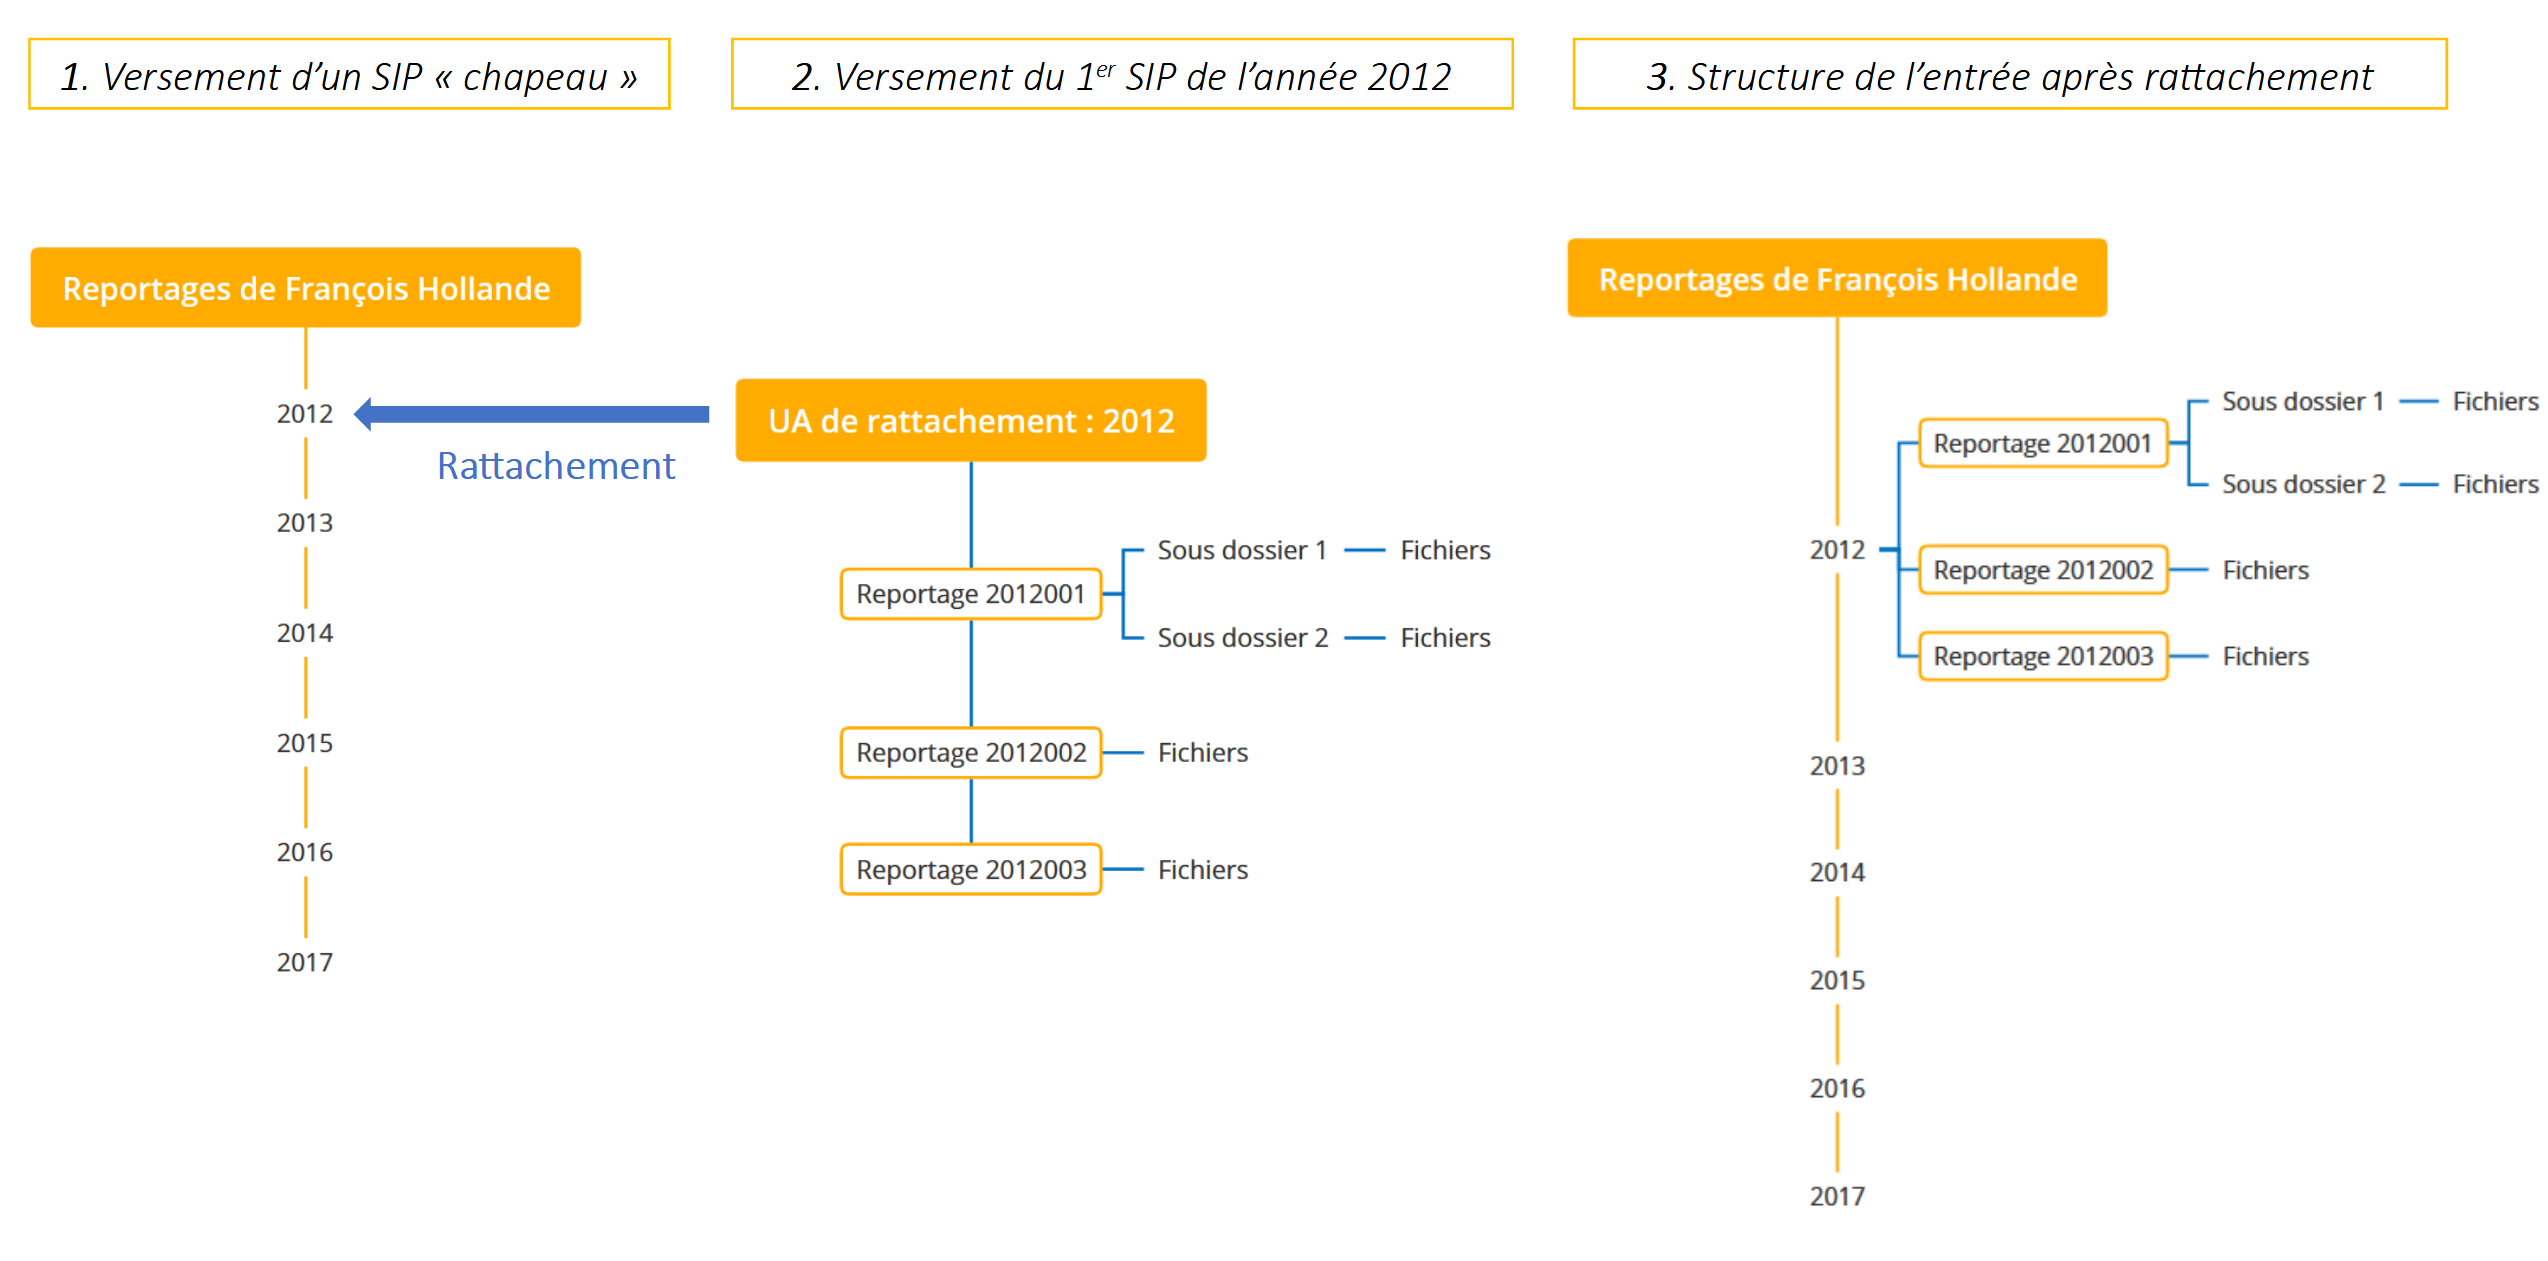
\includegraphics{./img/schema_rattachement.png}
	\end{adjustbox}
	\caption{Modélisation du processus de rattachement choisi pour les versements des reportages de la Présidence de la République.}
\end{figure}

Dans le cadre de la reprise des reportages photographiques, il était essentiel de comprendre non seulement le contexte institutionnel et technique de production des fichiers, mais aussi leur évolution depuis leur création jusqu'à leur reprise actuelle. En analysant l'impact de ce contexte de production sur la qualité des métadonnées descriptives, nous avons pu mettre en lumière tant les intérêts que les limites de leur utilisation dans un cadre archivistique. L'exemple de la collecte de reportages photographiques par la Bibliothèque nationale de France témoigne du fait que les défis rencontrés aux Archives nationales sont partagés par toutes des institutions patrimoniales confrontées à cette typologie documentaire.

Pour appréhender les exigences techniques auxquelles notre application devait répondre, il était indispensable de présenter l'environnement normatif et institutionnel de l'archivage électronique, ainsi que les traitements antérieurs appliqués dans le cadre des méthodes d'archivage précédentes. Les modifications introduites par le programme Constance ont, en effet, un impact direct sur la reprise des données, qui se décline en deux principales méthodes selon qu'il s'agisse de reportages traités ou non traités. Enfin, notre travail s'inscrit dans la méthodologie définie par le Département de l'administration des données pour l'ensemble du chantier de reprise des données. Cette méthodologie a été décrite, tout comme les contraintes spécifiques rencontrées dans le contexte très particulier de l'archivage électronique au sein du SAE Vitam des Archives nationales.

Tout ce travail de compréhension du contexte institutionnel et technique, de recherche des possibilités offertes par les technologies numériques, ainsi que la réflexion sur les enjeux archivistiques liés à la reprise de ce fonds, avait pour objectif de concevoir une méthode d'automatisation du traitement de ces reportages photographiques, garantissant ainsi leur accessibilité future. Dans la prochaine partie de ce mémoire, nous présenterons les réalisations concrètes effectuées au cours de ce stage, en particulier le pipeline de données, qui incarne l'aboutissement de cette méthode et sa mise en \oe{}uvre.

    \part{Conception d’un pipeline de données pour optimiser l’indexation des reportages photographiques}
	
\chapter{Analyse de l'existant : sources d'information et mappage des métadonnées}

Dans le cadre d'un projet de migration de données tel que la reprise des reportages photographiques, le mappage consiste à mettre en correspondance les champs de plusieurs sources d'informations, en faisant correspondre les champs sources avec les champs cibles. Dans le contexte de l'archivage électronique, il s'agit de définir les métadonnées que l'on souhaite fournir au SAE pour la gestion et l'accessibilité des données versées. La première étape consiste donc en la définition des métadonnées à transférer et l'identification des sources d'information que l'on va exploiter. Une connaissance approfondie du résultat attendu est également nécessaire pour que le mappage soit efficace. Ici, les métadonnées transmises au SAE sont embarquées dans le manifest exprimé en XML-SEDA ; il sera donc nécessaire d'établir des équivalences entre les métadonnées sélectionnées et les champs SEDA. Les difficultés rencontrées dans cette première étape ne sont pas sans rappeler celles que présente tout travail de traduction : existe-t-il une équivalence exacte entre le terme utilisé en langage naturel pour désigner l'information à transférer et le langage de destination, ici le SEDA ? Si une équivalence exacte ne peut être identifiée, il faut s'interroger sur la meilleure manière de le traduire en définissant précisément le signifiant afin de trouver le mot juste. Dans un second temps, une étape de transformation peut être nécessaire pour convertir les données d'un format à l'autre, ce qui implique un travail de nettoyage plus ou moins conséquent. Enfin, dans le contexte archivistique, le principe de non redondance de l'information implique un processus de réflexion qui permettra de déterminer le niveau de granularité associé à chaque métadonnée.

\section{Identifier les sources d'information (fiabilité, facilité d'utilisation) et les informations souhaitées}
\subsection*{De l'importance des données structurées : choisir les sources de métadonnées}
Si certaines informations sont requises lors de l'écriture du manifest SEDA, notamment des métadonnées de gestion, d'autres sont facultatives et sont ajoutées pour améliorer l'accessibilité des archives dans le SAE. Afin de déterminer les métadonnées descriptives susceptibles d'être utilisées, il est nécessaire de procéder à une analyse des données à notre disposition et de leur qualité. Dans le cadre de la reprise des reportages photographiques de la Présidence de la République, nous pouvons diviser les métadonnées à ajouter au manifest en trois catégories : les métadonnées externes issues de l'instrument de recherche, ou des autres documents décrivant le fonds, les métadonnées internes des photographies extraites avec Exiftool, et les métadonnées à créer.

Les instruments de recherche décrivent chaque article du versement, la description est donc réalisée au niveau du reportage. Ils contiennent les métadonnées suivantes : numéro de versement, nom du service producteur, dates extrêmes du fonds, intitulé du fonds, numéro du reportage, nom du reportage, nom du ou des photographe(s), date du reportage, lieu(x) de la prise de vue (sauf pour les reportages de la mandature de Jacques Chirac). Les métadonnées internes des fichiers peuvent contenir : l'intitulé du fichier, sa date de prise de vue, le nom du photographe, le lieu de la prise de vue, l'intitulé du reportage, une légende de la photo, et une série de mots-clés. Parmi les métadonnées à créer, certaines doivent être rédigées manuellement, tandis que d'autres peuvent être calculées par des outils informatiques : les métadonnées de format, tout comme l'empreinte des fichiers, sont produites par l'application Siegfried. 

Les instruments de recherche des reportages photographiques de l'Élysée existent sous des formes différentes : celui de la mandature de Jacques Chirac a été encodé en XML-EAD, celui de la mandature de Nicolas Sarkozy existe sous la forme d'un fichier PDF créé à partir d'un tableau Excel, et celui de la mandature de François Hollande a été écrit directement au format Microsoft Word. Tous ces formats ne sont pas aussi facilement exploitables. Les données des instruments de recherche sous la forme de tableur ou de fichier en XML-EAD sont dites \enquote{structurées}, c'est à dire qu'elles sont organisées de manière à être facilement identifiables et exploitables par un programme, elles ont une structure bien définie (tables, champs, balises) qui facilite leur traitement. Les données issues des instruments de recherche au format Microsoft Word ou PDF sont dites \enquote{non structurées}, elles sont plus difficiles à exploiter directement par un programme, l'information étant fournie en format libre (plein texte), ce qui complique l'extraction automatisée des données. Fort heureusement, pour les reportages de la mandature de François Hollande, un export CSV de la base de données Cindoc utilisée par le services des archives de l'Élysée fournit de manière beaucoup plus caractérisée les métadonnées descriptives attendues : numéro du reportage, intitulé, date de début et de fin, mots-clés, noms des personnalités identifiées, mots-clés géographiques (lieux de prise de vue ou liés thématiquement au reportage).

\subsection*{La donnée pivot, fil d'Ariane du pipeline de données}
Pour s'assurer que les bonnes métadonnées sont associées aux bonnes unités d'archives\footnote{En SEDA, l'unité d'archive correspond à une subdivision intellectuelle dans un instrument de recherche, alignée sur un niveau de description en ISAD-G. L'unité d'archives regroupe un ensemble de métadonnées destinées à décrire ou qualifier un document ou un ensemble de documents, permettant ainsi de gérer la hiérarchie intellectuelle tout en intégrant les métadonnées de description et de gestion spécifiques à chaque niveau archivistique.}, il est nécessaire d'identifier une donnée pivot, qui permettra de connecter les différentes sources de métadonnées aux unités d'archive correspondantes. Pour chaque reportage, cette donnée pivot est le numéro qui lui a été attribué par le service photographique, présent dans le titre du dossier contenant les fichier et dans l'instrument de recherche. Cependant, il a fallu faire preuve de vigilance, car de légères variations, telles que \enquote{1234B}, \enquote{1234Bis} ou \enquote{1234 Bis}, peuvent rendre cette donnée pivot inefficace.

Le nom du fichier ne constitue pas une valeur pivot fiable pour les photographies, car il peut être partagé par plusieurs fichiers au sein d'un même versement. Pour résoudre ce problème, nous avons alterné entre deux valeurs pour associer les métadonnées extraites par Exiftool et celles calculées par Siegfried aux objets de données. Nous avons utilisé soit l'empreinte unique du fichier, soit son chemin, car, dans la mesure où deux fichiers d'un même dossier ne peuvent avoir le même nom, le chemin est nécessairement propre à chaque fichier.

\section{Répartition des métadonnées par niveau de description}
Afin de garantir une description pertinente et fiable, une analyse approfondie des métadonnées était nécessaire. Celle-ci avait notamment pour objectif de définir à quel niveau de description archivistique chaque métadonnée descriptive devait être associée. En effet, chaque versement pouvait contenir entre quatre et cinq niveaux de description : l'unité archivistique (UA) racine (\enquote{Les reportages de X}), le millésime, le reportage, la séquence (en cas d'une division du reportage en plusieurs parties), et la photographie.

Nos réflexions ont surtout porté sur les UA de niveau \enquote{Reportage} et \enquote{Photographie}, notre objectif étant centré sur l'accessibilité du contenu intellectuel du fonds. Dans le chapitre 4, nous avons évoqué que toutes les métadonnées relatives aux reportages ou aux photographies ne seraient pas retenues pour l'indexation dans le SAE des Archives nationales. Le travail de mappage présenté ici s'inscrit dans cette perspective de sélection des informations à reprendre. Les UA de niveau \enquote{Année} et \enquote{Séquence} servent surtout à structurer le fonds, en particulier la première qui permet d'éviter que les centaines, voire milliers, de reportages apparaissent en râteau sous l'UA racine. 

La description archivistique repose sur plusieurs principes clés : le respect du fonds, la présentation du général au particulier, et la non redondance des informations d'un niveau à l'autre\footcite{isad2000}. Selon ce dernier principe, une métadonnée descriptive associée à un niveau haut s'applique nécessairement aux niveaux inférieurs. Ainsi, si nous savons que l'ensemble des photographies d'un reportage ont été prises par un même photographe, cette information peut être associée à ce niveau de description et sera appliquée à l'ensemble des unités de niveau inférieur. Cependant, si plusieurs photographes sont associés à un même reportage, il est préférable de distinguer lequel est responsable de chaque cliché et donc de placer l'information au niveau de la photographie. L'analyse des métadonnées internes des fichiers a révélé un nombre important de reportages multi-photographes, nous avons donc choisi de placer cette information au niveau des photographies. Il en va de même pour les métadonnées de localisation : bien que de nombreux reportages se déroulent dans un seul lieu, certains couvrent plusieurs lieux distincts et nécessitent une description plus détaillée à un niveau inférieur. Il convient toutefois de rappeler que l'idéal archivistique de non-redondance des informations est difficile à appliquer aux SAE, où les informations d'indexation sont stockées dans des bases de données. En effet, dans une base de données, l'indexation est souvent redondante afin de garantir la pertinence des résultats lors d'une requête.

Des questionnements similaires se sont imposés pour les métadonnées de description et d'indexation (mots-clés). Ces informations tirées des métadonnées internes sont donc censées correspondre à un niveau de granularité fin et apporter des informations propres à chaque prise de vue. Cependant, en 2023, l'analyse des métadonnées internes des reportages photographiques des services du Premier ministre a révélé que ces métadonnées étaient peu présentes et avaient pu être renseignées en masse et se répéter de manière identique dans toutes les photographies d'un reportage. Nous avions alors choisi de faire remonter les mots-clé au niveau des reportages afin d'éviter de créer du bruit dans une recherche par mots-clés, en faisant remonter des fichiers mal indexés. Lorsque la granularité de la description est fine, il est nécessaire de s'assurer de la fiabilité des informations. La situation était différente pour les reportages de la Présidence de la République : le service photographique disposant d'un iconographe, les métadonnées renseignées sont plus précises et plus riches. Nous avons donc choisi de conserver cette information à ce niveau de description.

\section{Le mappage des métadonnées en XML-SEDA : équivalences exactes et traductions contextuelles}

Les deux tableaux ci-dessous présentent le mappage réalisé pour les niveaux de description \enquote{Reportage} et \enquote{Photographie}.

\begin{table}[h]
	\centering
	\begin{tabularx}{\textwidth}{|m{4cm}|m{3.5cm}|m{7.2cm}|}
		\hline
		\rowcolor{pastelblue-dark} 
		\textbf{Information} & \textbf{Source} & \textbf{Balise SEDA} \\
		\hline
		\rowcolor{pastelblue}
		Numéro de reportage & CSV Cindoc & OriginatingAgencyArchiveUnitIdentifier \\
		\hline
		\rowcolor{pastelblue}
		Date & CSV Cindoc & StartDate et EndDate \\
		\hline
		\rowcolor{pastelblue}
		Niveau de description & À créer & DescriptionLevel \\
		\hline
		\rowcolor{pastelblue}
		Nom du reportage & CSV Cindoc & Title \\
		\hline
	\end{tabularx}
	\caption{Mappage des métadonnées associées aux unités d'archives de niveau \enquote{Reportage}.}
\end{table}

\begin{table}[h]
	\centering
	\begin{tabularx}{\textwidth}{|m{4cm}|m{4cm}|X|}
		\hline
		\rowcolor{pastelblue-dark} 
		\textbf{Information} & \textbf{Source} & \textbf{Balise SEDA} \\
		\hline
		\rowcolor{pastelblue}
		Intitulé du fichier & Nom du fichier avec extension & Title \\
		\hline
		\rowcolor{pastelblue}
		Date de prise de vue & Métadonnées internes & StartDate et EndDate \\
		\hline
		\rowcolor{pastelblue}
		Photographe (nom) & Métadonnées internes & AuthorizedAgent/FullName \\
		\hline
		\rowcolor{pastelblue}
		Photographe (activité) & À créer & AuthorizedAgent/Activity \\
		\hline
		\rowcolor{pastelblue}
		Photographe (type de contrat) & À créer & AuthorizedAgent/Mandate \\
		\hline
		\rowcolor{pastelblue}
		Légende & Métadonnées internes & Description \\
		\hline
		\rowcolor{pastelblue}
		Lieu de la prise de vue & Métadonnées internes & Coverage/Spatial \\
		\hline
		\rowcolor{pastelblue}
		Mots-clés & Métadonnées internes & Tag \\
		\hline
		\rowcolor{pastelblue}
		Niveau de description & À créer & DescriptionLevel \\
		\hline
	\end{tabularx}
	\caption{Mappage des métadonnées associées aux unités d'archives de niveau \enquote{Photographie}.}
\end{table}

Comme nous l'évoquions plus haut, le mappage est également un travail de traduction qui nécessite de se plonger dans le dictionnaire du langage cible pour éviter les contre-sens. 

Le numéro de reportage a été associé à la balise \enquote{OriginatingAgencyArchiveUnitIdentifier}, définit par le dictionnaire du SEDA comme \enquote{l'identifiant attribué à l’unité d’archives par le service producteur}\footcite{siafseda}En effet, le numéro de reportage n'est pas une cote déterminée par un service d'archives mais bien un identifiant créé par le service photographique. À l'exception des reportages de la mandature de Jacques Chirac, les fonds de reportages photographiques de la Présidence de la République ne sont en effet pas cotés à l'article : le seul identifiant dont nous disposons est donc le numéro de reportage. Une nouvelle cote leur sera attribuée au moment du versement dans le SAE : nous présenterons le processus de création de ces cotes dans le chapitre suivant.

Les noms de reportages et intitulés de fichiers sont associés à la balise \enquote{Title}, équivalence exacte s'il en est. Il en va de même pour les légendes des photographies, renvoyées vers la balise \enquote{Description}, et des mots-clés vers les balises \enquote{Tag}. Les champs de localisation sont divisées en deux (\enquote{City} et \enquote{Country}) dans les schéma de métadonnées d'images numériques (XMP, IPTC, Exif). En revanche, en SEDA, ces informations sont associées à la balise \enquote{Coverage} qui permet d'indexer les unités d'archives en fonction de leur couverture spatiale, temporelle ou juridictionnelle. Le type de couverture est précisé par l'élément enfant \enquote{Spatial}.

Nous avons rencontré plus de difficultés pour déterminer la balise permettant de retranscrire l'identité du photographe. En effet, la notion d'auteur, au sens de créateur d'une \oe{}uvre de l'esprit, n'existe pas en SEDA. Dans le contexte archivistique, cette notion est plutôt associée à celle de producteur, or dans le cas présent il s'agit du service photographique et non des agents qui le composent. Pour désigner l'auteur au sens de \enquote{rédacteur du document}, il existe un élément \enquote{Writer}, mais qui s'applique peu au contexte de la photographie. Nous nous sommes donc interrogés sur le sens que nous souhaitions faire porter à cette information : pourquoi souhaitons-nous faire apparaître le nom du photographe ? Pour respecter son droit moral et s'assurer qu'il soit crédité en cas de réutilisation de son \oe{}uvre. Il existe un élément SEDA \enquote{AuthorizedAgent} qui sert à désigner une \enquote{personne ayant des droits sur l’unité d’archives}. Voilà qui correspond davantage à notre situation. Il reste à préciser la nature de ces droits. L'élément \enquote{Activity} indique la profession du détenteur de droit (ici \enquote{Photographe}), et l'élément \enquote{Mandate} précise le \enquote{mandat octroyé à la personne} par exemple le \enquote{contrat de cession de droits en termes de propriété intellectuelle et artistique sur une archive}. En précisant dans la balise \enquote{Mandate} qu'il s'agit d'un photographe de l'Élysée et non d'un photographe privé, nous caractérisons la nature du lien entre l'archive et le photographe : en tant qu'agent de service public, il détient un droit moral sur son \oe{}uvre, mais pas de droits patrimoniaux et n'a pas à être consulté en cas de diffusion de la photographie.
\\

Dans ce chapitre, nous avons présenté les critères et les méthodes qui ont orienté notre sélection des métadonnées descriptives utilisées pour la reprise des reportages photographiques, dans le but d'améliorer leur indexation et leur accessibilité au sein du SAE des Archives nationales. Comme indiqué dans les chapitres précédents, cette démarche vise à compenser l'absence de description archivistique en utilisant les métadonnées fournies par le service photographique de la Présidence. Toutefois, cette contrainte ne nous exonère pas de la responsabilité de garantir la fiabilité des métadonnées intégrées. Malgré la nécessité de s'adapter aux données disponibles, il est impératif de veiller à la qualité et à la précision des informations choisies, ainsi qu'à leur conformité aux normes archivistiques. En somme, bien que l'adaptation aux contraintes pratiques soit inévitable, une approche vigilante et rigoureuse demeure essentielle pour maintenir l'intégrité et la valeur des archives que nous traitons. La documentation précise de la provenance des métadonnées intégrées dans cette reprise constitue une première réponse à ces exigences, garantissant ainsi une traçabilité et une transparence dans le traitement archivistique des données.
\chapter{Conception du pipeline de données}
\section{Définir les objectifs de l'application}

L'outil produit dans le cadre de mon stage de Master 2 au Département de l'administration des données des Archives nationales est une application ayant pour fonction la fabrication de paquets d’archives (SIP) pour la reprise des reportages photographiques de la Présidence de François Hollande en vue de leur versement dans le SAE Vitam des Archives nationales. Baptisée ORPhÉE (Outil de Reprise de Photographies et Éléments Embarqués), son intérêt principal réside en sa capacité à extraire les métadonnées internes des photographies, notamment les métadonnées descriptives qui ont pu être renseignées par le photographe (description, mots-clés, nom du photographe, lieux de la prise de vue). Le deuxième enjeu était de s'assurer que l'application permettait bien de restituer l'arborescence des reportages après leur versement. 

ORPhÉE devait donc produire un bordereau de versement conforme au SEDA (manifest) restituant la structure intellectuelle des reportages et enrichi des métadonnées internes des photographies et des métadonnées externes des reportages issues de l'export CSV de la base Cindoc des archives de l'Élysée. La création du manifest devait s'accompagner de la copie à plat et du renommage de l'ensemble des fichiers ajoutés au paquet dans un dossier \enquote{content}. 

La majeure partie de mon travail a consisté en la création du manifest : c'est en effet lui qui fournira au SAE les informations de structure et de description qui permettront l'affichage et l'accessibilité des fichiers archivés. Une brève présentation de la structure d'un manifest semble donc de rigueur afin de comprendre au mieux le processus de création de l'application ORPhÉE. Cette structure est synthétisée par la Figure 8.1 à la page suivante.

\begin{figure}
	\centering
	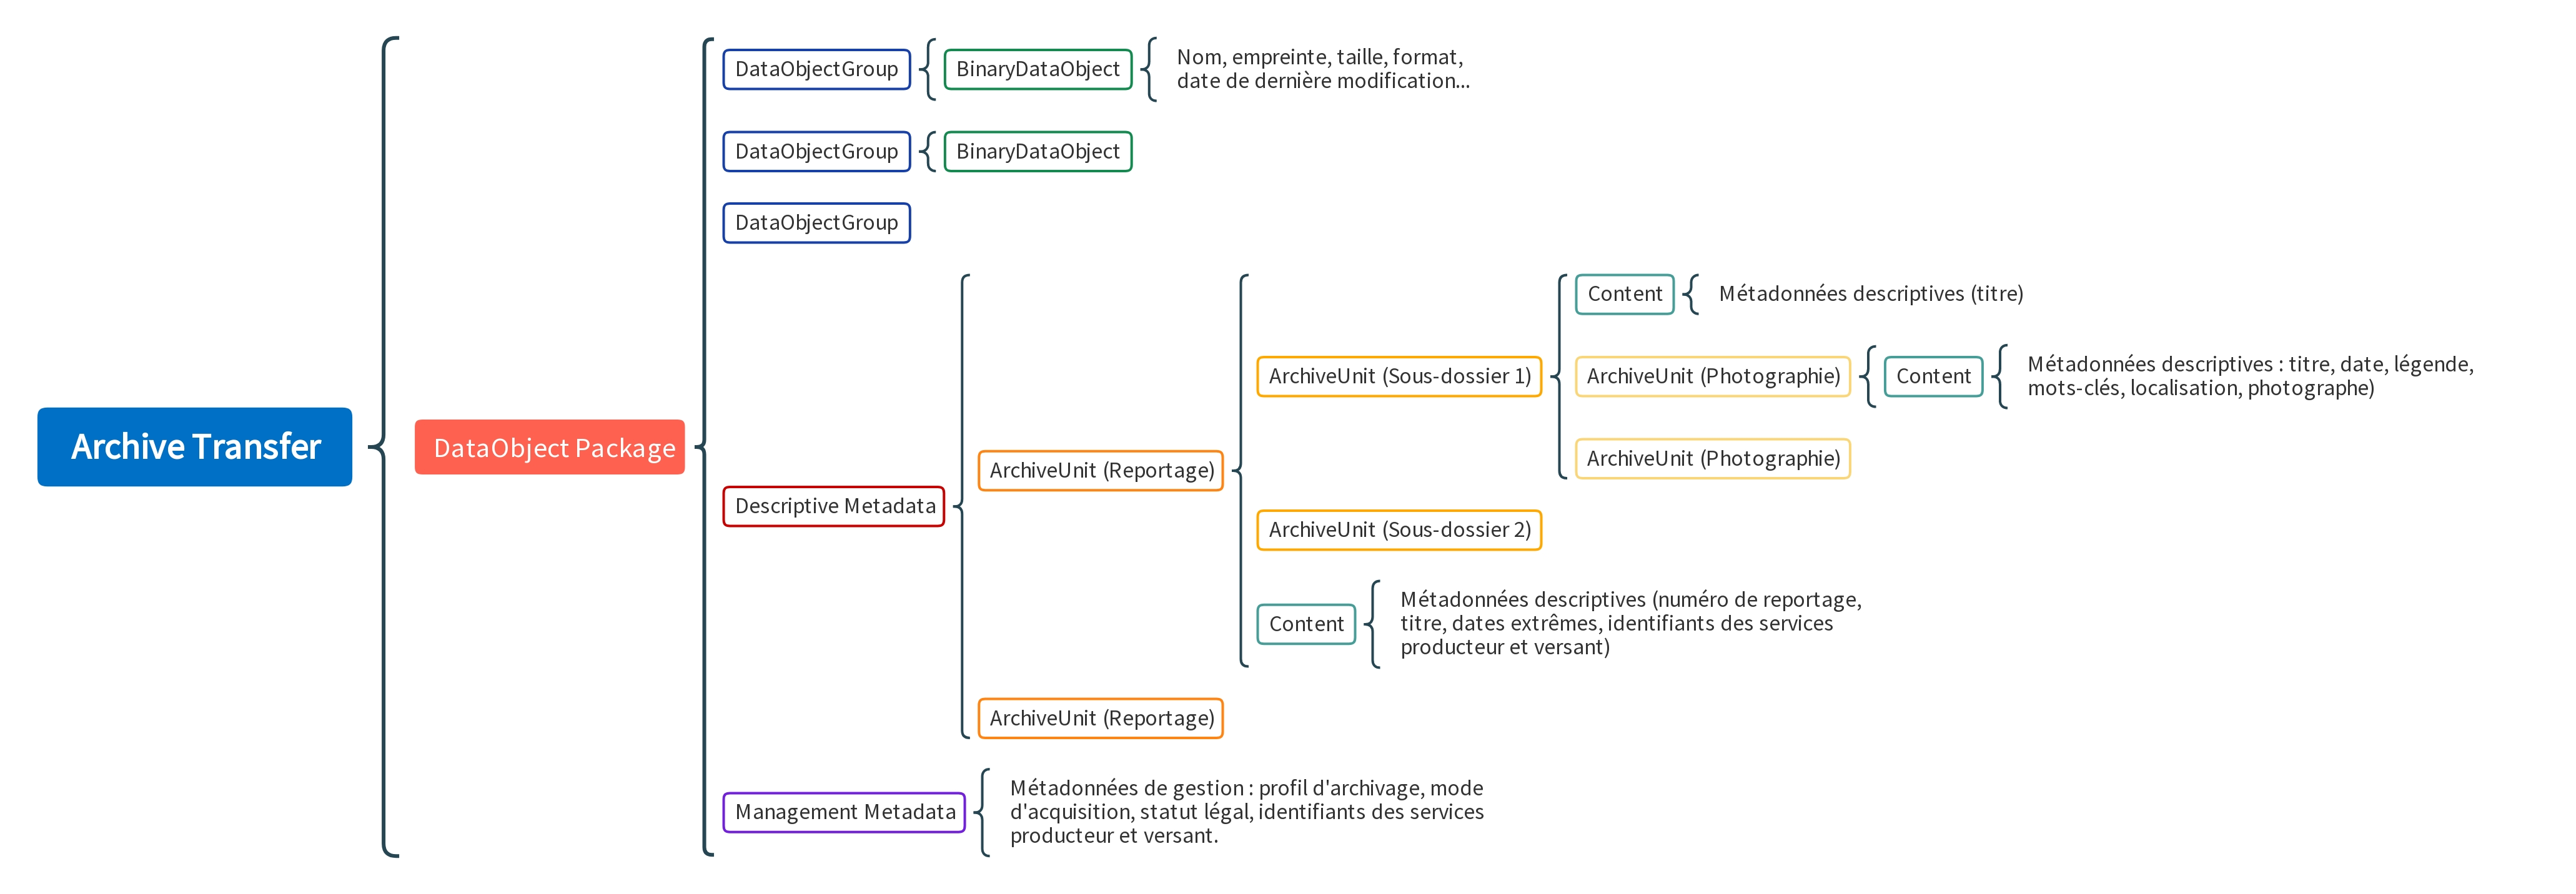
\includegraphics[angle=90, height=\dimexpr\textheight-2cm\relax]{./img/ArchiveTransfer.jpg}
	\caption{Schéma présentant les principales sections du manifest en SEDA produit par l'application ORPhÉE, ainsi que leur contenu.}
\end{figure}

\newpage
Le manifest est un document XML dont la racine est l'élément \xmlinline{<ArchiveTransfer>}. Il est composé d'un en-tête qui fournit l'identifiant du paquet d'archives et des informations techniques liées aux modalités de versement, et d'un élément \xmlinline{<DataObjectPackage>} qui contient les métadonnées techniques, descriptives et de gestion relatives aux archives constitutives du paquet. Nous nous intéresserons donc particulièrement au contenu de cet élément. Il se divise en trois grands blocs : une succession d'éléments \xmlinline{<DataObjectGroup>}, un élément \xmlinline{<DescriptiveMetadata>}, et un élément \xmlinline{<ManagementMetadata>}. Chaque \xmlinline{<DataObjectGroup>} correspond à un document dans toutes ses versions (originaux, diffusion, version textuelle). Ainsi, en SEDA, un même document peut être représenté par plusieurs fichiers, chacun étant associé à un élément \xmlinline{<BinaryDataObject>} : dans notre cas, chaque document correspond à un seul fichier, l'original,  chaque \xmlinline{<DataObjectGroup>} est donc composé d'un seul \xmlinline{<BinaryDataObject>}. Cet élément contient des métadonnées techniques relatives au fichier : empreinte, format, date de dernière modification, taille... L'élément \xmlinline{<DescriptiveMetadata>} permet de restituer la structure du versement ainsi que les métadonnées descriptives associées à chaque unité d'archives, ou \xmlinline{<ArchiveUnit>}. L'élément \xmlinline{<ManagementMetadata>} contient quant à lui les métadonnées de gestion communes à l'ensemble du paquet. Pour bien associer chaque \xmlinline{<DataObjectGroup>} à l' \xmlinline{<ArchiveUnit>} correspondant, un jeu d'identifiants est mis en place au sein du manifest. Les fichiers copiés dans le paquet correspondant aux éléments \xmlinline{<BinaryDataObject>}, ils sont renommés en utilisant les identifiants associés à ces éléments.

\section{Fonctionnement de l'application}

\subsection*{Collecte des données et métadonnées nécessaires}
Pour fonctionner correctement, l'application doit ingérer un certain nombre d'informations qui serviront ensuite à enrichir le manifest, à sélectionner les reportages à ajouter au paquet, ou à définir les modalités de rattachement dans le SAE. Certaines informations, communes à tous les paquets de reportages photographiques de la Présidence, sont inscrites \enquote{en dur} dans l'application : l'utilisateur n'a pas besoin de les renseigner. C'est le cas par exemple des métadonnées de gestion du \xmlinline{<ManagementMetadata>}. D'autres informations sont relatives au paquet et sont demandées à l'utilisateur au lancement de l'application : numéro d'entrée, numéro du paquet, méthode de rattachement... Enfin, la plupart des informations sont issues de fichiers externes ou des photographies elles-mêmes.

\subsubsection*{Import des fichiers de données}

L'application prend deux fichiers en entrée : le CSV contenant les métadonnées descriptives externes des reportages, et la liste au format texte des reportages à ajouter au paquet. ORPhÉE transforme l'export CSV de la base Cindoc en listes de données : chaque ligne du tableau correspondant à une liste des métadonnées descriptives de chaque reportage (numéro, titre, dates extrêmes), toutes ces listes sont réunies dans une grande liste qui correspond au fichier CSV dans son ensemble. Le contenu du fichier texte est également transformé en une liste de numéros de reportages : cette liste est utilisée tout au long du traitement pour vérifier à toutes les étapes que seuls les reportages sélectionnés sont inclus au paquet.

\subsubsection*{Extraction des métadonnées internes et calcul des métadonnées de format}

Trois étapes du pipeline permettent l'exploitation des métadonnées internes des fichiers. La librairie PyExiftool est utilisée pour extraire les métadonnées internes des fichiers selon les mêmes modalités qu'Exiftool. La commande Python est par ailleurs très proche de celle utilisée en ligne de commande avec l'application lorsqu'elle est appelée dans le terminal : précision du format attendu pour la restitution des données extraites (JSON), commande d'itérer dans les sous-dossiers du répertoire analysé, liste des métadonnées à extraire, puis chemin du répertoire à analyser (représenté ici par la variable \enquote{item\_path}). J'ai rencontré de nombreux problèmes d'encodage lors de l'extraction des métadonnées, les caractères spéciaux n'étant pas restitués correctement, il était en effet nécessaire d'expliciter à presque chaque étape du pipeline l'encodage des chaînes de caractères manipulées (ici, l'UTF-8).
 \\
\begin{python}
exif_data_list = et.execute_json('-r', '-b', '-FileName', '-CreateDate', '-By-line', '-Artist', '-City', '-Country',
'-Country-PrimaryLocationName', '-Description', '-Subject', '-Keywords', '-FileModifyDate', '-Filesize#', item_path)
\end{python}

Le logiciel Siegfried est ensuite utilisé pour produire les métadonnées de format et calculer l'empreinte, l'ensemble de ces informations est également fourni au format JSON. Les métadonnées collectées au cours de ces deux étapes n'étaient cependant pas réunies au sein d'une même variable JSON, ce qui ralentissait considérablement l'application qui devait parcourir deux sources d'information pour récupérer les métadonnées associées à un même fichier. Pour simplifier ce processus, j'ai ajouté une étape dont l'objectif était de fusionner les deux sources de métadonnées : l'application parcourt d’abord les métadonnées issues de Siegfried et identifie les chemin de tous les fichiers. Elle cherche ensuite le même chemin dans les métadonnées extraites par Exiftool. Lorsqu’une correspondance est trouvée, la fonction fusionne les métadonnées Exiftool et Siegfried pour que l’ensemble des métadonnées d’un même fichier soient stockées au même endroit.
\\

À l'issue de cette première étape, l'ensemble des métadonnées nécessaires a été identifié, extrait et stocké. L'étape suivante d'écriture du manifest permettra des les associer aux objets de données (fichiers) et aux unités archivistiques correspondantes.

\subsection*{Écriture du manifest}
Pour l'écriture des éléments du manifest en XML, j'ai utilisé la librairie Python ElementTree. Elle permet de créer, organiser et écrire des fichiers XML en proposant des outils pour définir des balises, ajouter des sous-éléments, et sauvegarder la structure XML dans un fichier. Dans un premier temps, l’élément racine du manifest et les éléments de l’en-tête sont créés. La majorité d'entre eux ont des valeurs fixes qui sont renseignées directement dans le code de l'application (noms des services producteur et versant, nom du service d'archives). Est ensuite créé l'élément \xmlinline{<DataObjectPackage>} dont le contenu sera écrit petit à petit au cours des étapes successives du pipeline de données.
\subsection*{Identifier les objets de données}

Pour créer les éléments \xmlinline{<DataObjectGroup>} et \xmlinline{<BinaryDataObject>}, l'application parcourt de manière récursive l’ensemble des fichiers des reportages sélectionnés : ces deux éléments sont créés pour chacun des fichiers identifiés. L'application est programmée pour ignorer les fichiers exclus de la reprise (fichiers système ou masqués) repérés à l'aide de leur nommage. Dans un second temps, l'application recherche les métadonnées techniques de ces objets de données calculées par Siegfried et les associe à chaque \xmlinline{<BinaryDataObject>}. Voici un extrait du manifest représentant ces éléments à ce point du traitement. On notera que certaines informations sont absentes à ce stade d'écriture du manifest.

\begin{xml}
<DataObjectGroup>
	<BinaryDataObject>
		<DataObjectVersion>BinaryMaster_1</DataObjectVersion>
		<Uri></Uri>
		<MessageDigest algorithm="SHA-512">775e48fa4c2bbc1838496ed992f0e653ee45412d1ad4b87f102c677ff1488cf02b0275d4dd84e3cf2c4e5870c3b44a4a3c181261fe20ebdf004eb164b30ba686</MessageDigest>
		<Size>6315358</Size>
		<FormatIdentification>
			<FormatLitteral>Exchangeable Image File Format (Compressed)</FormatLitteral>
			<MimeType>image/jpeg</MimeType>
			<FormatId>fmt/645</FormatId>
		</FormatIdentification>
		<FileInfo>
			<Filename>1304780002.JPG</Filename>
			<LastModified>2013-06-24T09:54:52</LastModified>
		</FileInfo>
	</BinaryDataObject>
</DataObjectGroup>
\end{xml}

En cas de doublons techniques, c'est à dire de fichiers complètement identiques, le SEDA permet de ne conserver qu’une seule version et de l’associer à chaque unité d'archive correspondante. Ainsi, lors de la restitution du versement dans le SAE, le fichier sera recréé partout où il était présent dans la structure des dossiers, mais il ne sera conservé physiquement qu’une seule fois. Cette opération n'est pas obligatoire, mais elle permet de réduire la taille du paquet. J'ai donc ajouté une étape de suppression des \xmlinline{<DataObjectGroup>} correspondant à des doublons techniques. L'application parcourt l’ensemble des \xmlinline{<DataObjectGroup>} créés et en mémorise l’empreinte. Si l’application repère une empreinte déjà identifiée, il s’agit d’un doublon : le \xmlinline{<DataObjectGroup>} en double (ou triple) est donc supprimé.

\subsubsection*{Reconstituer l'arborescence des reportages}

Après avoir listé les objets de données et leurs métadonnées techniques dans la première moitié du \xmlinline{<DataObjectPackage>}, l'application procède à la description des unités d'archive du versement dans l'élément \xmlinline{<DescriptiveMetadata>}. Comme pour la création des \xmlinline{<DataObjectGroup>}, l'application commence par identifier tous les dossiers correspondant à des reportages sélectionnés. Pour chacun d'entre eux, un élément \xmlinline{<ArchiveUnit>} est créé et enrichi avec des métadonnées de gestion et les métadonnées descriptives issues de l'export CSV de la base Cindoc : titre, numéro de reportage, dates extrêmes, etc.
Pour chaque \xmlinline{<ArchiveUnit>} créé (fichier ou dossier) une cote lui est attribuée en combinant le numéro d'entrée, le numéro du paquet, et une numérotation incrémentale de toutes les unités du paquet (ex : 20240001\_1\_135). Voici un extrait du manifest correspondant à la description d'une unité archivistique de niveau reportage : 

\begin{xml}
<ArchiveUnit>
	<Content>
		<DescriptionLevel>RecordGrp</DescriptionLevel>
		<Title>Interview pour France G, Palais de l'Elysée, Paris, 03 janvier 2013.</Title>
		<ArchivalAgencyArchiveUnitIdentifier>20240001_1_135</ArchivalAgencyArchiveUnitIdentifier>
		<OriginatingAgencyArchiveUnitIdentifier>130479</OriginatingAgencyArchiveUnitIdentifier>
		<Description>Reportage n°130479</Description>
		<OriginatingAgency>
			<Identifier>FRAN_NP_009886</Identifier>
		</OriginatingAgency>
		<SubmissionAgency>
			<Identifier>FRAN_NP_009886</Identifier>
		</SubmissionAgency>
		<StartDate>2013-01-03T00:00:00</StartDate>
		<EndDate>2013-01-03T00:00:00</EndDate>
	</Content>
\end{xml}

L'une des principales difficultés rencontrées pour la création de cette partie du manifest est liée à la restitution de la structure des reportages à partir de l'arborescence des dossiers : toutes les unités archivistiques s'imbriquaient les unes dans les autres, ou encore ne s'imbriquaient pas du tout. Après avoir essuyé de nombreux échecs, j'ai identifié une solution qui consistait à faire boucler sur elle-même l'étape d'identification des sous-dossiers et des fichiers jusqu'à l'épuisement du nombre de niveaux d'arborescence. Voici un extrait de la fonction qui explore chaque dossier et appelle deux autres fonctions pour renseigner les métadonnées descriptives de chaque unité d'archive identifiée : 
\\
\begin{python}
# Parcourir les éléments (fichiers et sous-répertoires) dans le répertoire spécifié
for item in os.listdir(directory):
	# Si l'élément est un répertoire, créer une sous-unité d'archive et appeler la fonction qui ajoutera les métadonnées descriptives
	item_path = os.path.join(directory, item)
	if os.path.isdir(item_path):
		sub_archive_unit = ET.SubElement(archiveunit, "ArchiveUnit")
		contentsub = create_archive_unit_dir(item)
		# Appel récursif de la fonction pour traiter les sous-répertoires
		sub_unit(item_path, data, data_ir, liste_rp, sub_archive_unit)
	# Si l'élément est un fichier, appeler la fonction qui crée l'unité d'archive de niveau "fichier"
	elif (os.path.isfile(item_path)):
		file_unit = create_archive_unit_file(item, data, item_path)
\end{python}

La méthode suivie par l'application peut être mieux appréhendée à travers une analogie : imaginons un catalogueur nommé Orphée, chargé d'inventorier une collection (le fonds) de poupées russes (les reportages). Chaque poupée peut contenir d'autres poupées (les sous-dossiers), qui elles-mêmes peuvent renfermer encore d'autres poupées (deuxième niveau de sous-dossiers), ou parfois des objets individuels (les fichiers). Initialement, Orphée a tenté d'organiser ces poupées en se concentrant sur chaque niveau séparément : il a commencé par ranger toutes les grandes poupées ensemble, puis les moyennes, et enfin les petites. Cependant, au lieu d'obtenir une structure cohérente, il s'est retrouvé avec des poupées mal imbriquées : certaines étaient imbriquées indéfiniment, tandis que d'autres restaient à l'extérieur, non reliées aux autres. Il traitait chaque poupée et son contenu indépendamment, sans vraiment tenir compte des relations entre elles. Finalement, il a réalisé que la clé pour une imbrication correcte était de considérer chaque poupée comme une partie d'un ensemble : il devait ouvrir chaque grande poupée, puis examiner son contenu. Lorsqu'il trouvait une autre poupée, il l'ouvrait également, et ainsi de suite, jusqu'à atteindre les objets individuels à l'intérieur. Il a donc adopté une méthode où il ouvrait chaque poupée trouvée, vérifiait son contenu, et répétait ce processus jusqu'à ce que toutes les poupées soient parfaitement imbriquées. En somme, Orphée a opté pour une approche où chaque poupée était traitée immédiatement, avec une répétition de l'opération pour chaque contenu, ce qui a permis de restituer une structure hiérarchique correcte, avec chaque poupée à sa place, imbriquée dans une autre, de la plus grande à la plus petite.

\subsubsection*{Répartition des métadonnées internes et adaptation au SEDA}

Une fois l'ensemble des éléments \xmlinline{<ArchiveUnit>} créés, l'application récupère les métadonnées descriptives des fichiers extraites avec PyExiftool\footnote{Voir la documentation de la librairie PyExiftool : \url{https://pypi.org/project/PyExifTool/}.} et les place dans les bonnes balises SEDA, tel qu'évoqué dans le mappage du chapitre précédent. Une fois que le bon fichier a été identifié à l'aide d'une valeur pivot (le chemin du fichier), il s’agit uniquement de récupérer les métadonnées souhaitées et de les placer dans l’élément correspondant. Lorsque plusieurs champs de métadonnées peuvent correspondre à une même information, un champ est utilisé en priorité. Par exemple, pour les mots-clés, l’application utilise en priorité les informations renseignées dans le champ Subject du schéma XMP. Si ce champ est vide, elle interroge le champ Keywords du schéma IPTC. Cette opération est répétée pour l’ensemble des métadonnées choisies (description, mots-clés, localisation, nom du photographe, date de création). L'ordre de priorité a été établi en amont en identifiant les champs les mieux renseignés lors de l'analyse des données. 

Si la plupart des métadonnées extraites peuvent être restituées telle quelle dans le manifest, certaines doivent être modifiées pour répondre aux exigences du SEDA. C'est pas exemple le cas des dates. En SEDA, les dates doivent suivre le format suivant : aaaa-MM-jjTHH:mm:ss. Or, dans l'export CSV de la base Cindoc, elles sont exprimées dans un autre format (jj.MM.aaaa), et encore dans un autre dans les métadonnées internes des photographies (aaaa:MM:jj HH:mm:ss). Il était donc nécessaire d'adapter le format fourni pour qu'il soit conforme aux exigences d'un manifest SEDA. J'ai donc recouru à des expressions régulières pour modéliser chaque format de date, puis à des déplacements et remplacements pour obtenir le format souhaité, pour les fichiers...

\begin{python}
	# Expression régulière pour isoler les éléments de date qu'on souhaite récupérer
	match = re.match(r"(\d{4}:\d{2}:\d{2}\s\d{2}:\d{2}:\d{2})(\.\d+)?([-+]\d{2}:\d{2})?",
	createdate)
	if match:
	# Match sur le groupe 1 de l'expression régulière
	createdate = match.group(1)
	# Définition du format de date actuel
	createdate = datetime.strptime(createdate, "%Y:%m:%d %H:%M:%S")
	# Transformation vers le format de date souhaité
	createdate = createdate.strftime("%Y-%m-%dT%H:%M:%S")
\end{python}

... et pour les reportages.

\begin{python}
	dtf = datetime.strptime(RP[3], "%d.%m.%Y")
	dtf = dtf.strftime("%Y-%m-%dT%H:%M:%S")
\end{python}



\subsubsection*{Création des identifiants et association des unités d'archives aux objets de données}
La phase finale de l'élaboration du manifest consiste à associer les unités archivistiques aux groupes d'objets techniques (fichiers) correspondants. Pour ce faire, un identifiant unique est attribué de manière incrémentale à chaque élément : \xmlinline{<DataObjectGroup>} (GOT1, GOT2, etc.), \xmlinline{<BinaryDataObject>} (BDO1, BDO2, etc.) et \xmlinline{<ArchiveUnit>} (AU1, AU2, etc.). Ensuite, l'application parcourt le manifest pour établir un lien entre chaque \xmlinline{<ArchiveUnit>} et l'identifiant du \xmlinline{<DataObjectGroup>} correspondant. Cette association est réalisée à l'aide de l'empreinte numérique, qui joue ici un rôle de donnée pivot. Bien qu'elle ne soit pas directement une métadonnée des unités archivistiques, une balise temporaire a été créée spécifiquement pour cette étape, assurant ainsi une donnée commune entre les différents éléments à associer. A l'issue de cette étape, la balise est supprimée. Ces associations d'identifiants garantissent la cohérence des liens entre les unités d'archives et les objets binaires.

\subsection*{Copie et renommage des fichiers dans le dossier \enquote{content}}

L'application procède au transfert final des fichiers vers un répertoire cible en utilisant les empreintes numériques pour établir la correspondance avec les éléments décrits dans le manifest. D'abord, elle crée un dossier nommé \enquote{content} dans le même répertoire où sera généré le manifest, destiné à recevoir les fichiers copiés. Pour chaque fichier (\xmlinline{<BinaryDataObject>}), elle extrait le nom original du fichier. Un nouveau nom est alors généré, basé sur l'identifiant unique assigné à l'objet de données (\xmlinline{<BinaryDataObject>}), tout en préservant l'extension du fichier d'origine. Enfin, les fichiers sont copiés à plat dans le répertoire cible sous leur nouvelle dénomination. Le répetoire cible contient désormais le manifest en XML et un dossier \enquote{content} dans lequel se trouvent tous les fichiers des reportages sélectionnés : le paquet est prêt !\footnote{Voir la modélisation du fonctionnement de l'application en annexe \ref{sec:annexe1}.}
	
\chapter{Maintenabilité et perspectives d'utilisations futures de l'application}

Initialement, ma mission consistait à produire une preuve de concept (\gls{poc}, ou PoC) pour l'automatisation du traitement des reportages photographiques de la Présidence. Cependant, le travail effectué a abouti à la création d'un outil capable de générer des paquets pour la reprise de ces reportages, répondant ainsi aux besoins immédiats du service. Ce n'est qu'après la production de cet outil que nous avons pris conscience de son potentiel pour d'autres fonds photographiques aux Archives nationales, ainsi que pour d'autres services d'archives utilisant la solution logicielle Vitam. Nous nous sommes donc interrogés sur la réutilisabilité de l'application, pour d'autres services en l'état ou en l'intégrant à une autre application informatique.

\section{Utilisation dans un contexte différent : formulaire et guide d'utilisation}

Afin d'adapter l'application à des contextes d'utilisation différents, j'ai créé une version paramétrable, disponible sur mon Github\footnote{Le code des deux version a été déposé sur Github : \url{ https://github.com/SelmaKaina/ORPhEE/tree/main}.}. Grace à l'ajout d'une interface sous la forme d'un formulaire, cette version permet à l'utilisateur de renseigner un certain nombre d'informations qui étaient inscrites en dur dans le code de l'application originale (identifiants du service d’archives, du service producteur et du service versant, type de contrat des photographes). En raison des spécificités des paquets d'archives composés par l'outil, son usage n'est adapté qu'aux services utilisant la solution logicielle Vitam. L'application nécessite par ailleurs un nettoyage des données et la production d’un fichier de métadonnées externes selon des critères très spécifiques explicités dans un guide d'utilisation également mis en ligne.

Le formulaire est composé de 13 champs, tous obligatoires : 
\begin{figure}[h]
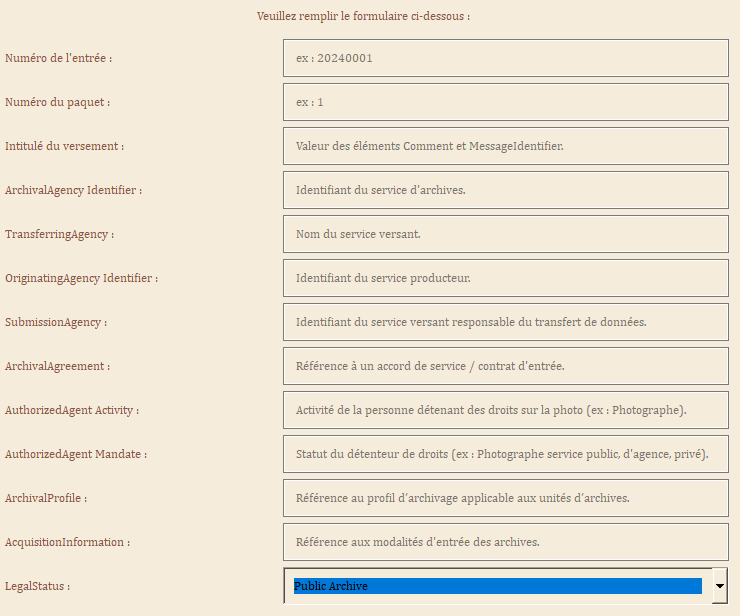
\includegraphics[width=\textwidth]{./img/orphee_formulaire_1.png}
\caption{Capture d'écran de la première partie du formulaire de l'application ORPhÉE.}
\end{figure}

Dans un second temps, le formulaire permet à l'utilisateur de choisir les métadonnées internes à extraire avec la librairie PyExiftool : chaque case cochée correspond à un champ de métadonnées que l’utilisateur souhaite extraire des fichiers pour l’ajouter au manifest. Nous évoquions dans le chapitre précédent la nécessité d'établir une priorité dans le choix des informations issues de plusieurs schémas de métadonnées : le guide utilisateur précise l'ordre établi pendant l'analyse des reportages de la Présidence de la République et adopté par l'application. Il est donc recommandé aux utilisateurs de procéder en amont à une analyse des métadonnées internes afin d'assurer une sélection des champs les plus pertinents. De plus, à l'instar de la première version de l'application, il est proposé de rattacher le paquet fabriqué à une unité archivistique déjà versée en cochant une case et en renseignant les informations nécessaires.

Le recours à ce formulaire permet notamment de revenir sur les informations renseignées, ce qui présente un avantage conséquent par rapport à la première version de l'application qui demandait les informations les unes après les autres et ne permettait pas de modifier une information déjà fournie.


\section{Pistes d'améliorations fonctionnelles}

\subsection*{Gestion des erreurs et validation du manifest}

L'application actuelle ne dispose pas encore d'un système de gestion des erreurs robuste. Par manque de temps, je n'ai pas pu intégrer un traitement interne des erreurs. Comme solution temporaire, j'ai répertorié les erreurs les plus fréquentes dans la documentation de l'application, en expliquant leur origine et en proposant des solutions possibles.

Par exemple, la présence de chemins trop longs ou de certains caractères spéciaux dans les noms de dossiers et de fichiers peut empêcher le bon fonctionnement de l'application, entraînant une erreur de balise vide. Les outils externes utilisés par l'application, tels que Siegfried et PyExiftool, ne reconnaissent pas ces chemins ou les excluent de leur traitement, ce qui peut provoquer deux types d'erreurs : une erreur lors de l'extraction des métadonnées, et une erreur lors de l'écriture du manifest. Lorsqu'un chemin contient un caractère spécial, il peut être mal interprété par l'application, qui ne parvient alors pas à retrouver le fichier dans l'arborescence. En conséquence, aucune métadonnée n'est récupérée, ce qui génère une erreur. Aussi, certains éléments associés aux fichiers dont le chemin pose problème ne sont pas créés, comme l'élément \xmlinline{<BaliseTemp>} qui devrait contenir l'empreinte calculée par Siegfried. Si cet élément n'est pas créé, l'application renvoie une erreur.

Une autre fonctionnalité que j'aurais souhaité pouvoir implémenter est la vérification de la validité du manifest en SEDA, avec une restitution des erreurs et des suggestions de solutions.

\subsection*{Optimisation des performances et scalabilité}

Une autre piste d'amélioration concerne l'optimisation du code : réviser l'ensemble des fonctions afin de déterminer s'il existe des opérations redondantes, ou des algorithmes complexes qui pourraient être simplifiés. Ces améliorations permettraient d'augmenter les performances de l'outil et de garantir qu'il puisse gérer une charge croissante de données sans perdre en efficacité.

La scalabilité désigne la capacité d'un système à s'adapter à une augmentation de la taille des données tout en maintenant des performances acceptables. Actuellement, la constitution d’un paquet de 20 Go prend entre 10 et 20 minutes, celle d’un paquet de 60 Go entre 20 et 30 minutes, et celle d’un paquet de 100 Go entre 40 minutes et 1 heure. Ce comportement linéaire du temps de traitement en fonction de la taille des données indique que le logiciel pourrait être optimisé pour améliorer la scalabilité.

\subsection*{Améliorations du formulaire}

Une autre amélioration possible serait l'ajout d'un fichier de configuration permettant de préremplir automatiquement certaines métadonnées dans le formulaire, en fonction du contexte d'utilisation. Par exemple, un service d'archives pourrait ainsi éviter de renseigner son identifiant à chaque utilisation de l'application.


\section{Maintenabilité de l'application}
L'application a été initialement conçue pour répondre à un besoin immédiat, ponctuel, et interne au Département de l'administration des données : l'automatisation de la reprise des reportages photographiques. L'objectif principal était donc de développer un outil qui reproduise les étapes définies lors de la modélisation du traitement des données. Ainsi, la pérennité de l'outil n'a pas été envisagée dès le départ. Une fois son efficacité avérée, la possibilité d'une utilisation par d'autres services d'archives a été envisagée. Cette nouvelle perspective nous a amené à nous interroger sur sa maintenabilité à l'issue du stage et du chantier de reprise. La notion de maintenabilité d'un logiciel renvoie à sa capacité à être facilement modifié, corrigé, ou amélioré au fil du temps. Elle dépend de la qualité du code, de sa modularité, de la clarté de la documentation, et de l'adoption de bonnes pratiques de développement.

Dans ce contexte, nous avons étudié les facteurs permettant de garantir la reprise de l'outil par d'autres utilisateurs. Chaque fonction a été documentée avec des \gls{docstrings}, avec l'ajout de commentaires spécifiques pour décrire les différentes étapes des fonctions les plus complexes. J'ai rédigé une documentation, mise en ligne sur GitHub. Cette documentation se divise en plusieurs parties: 

\begin{itemize}
	\item Un guide décrivant le format des données acceptées et les bonnes pratiques d'analyse et de nettoyage des données à réaliser en amont.
	\item Une présentation de l'interface utilisateur détaillant les différentes sections du formulaire et les messages de suivi des opérations.
	\item Une liste des erreurs les plus fréquentes, précisant leur origine et les moyens identifiés pour les solutionner.
	\item Une description du fonctionnement du code détaillant chacune des fonctions qui le constituent.
\end{itemize}

De plus, j'ai animé plusieurs réunions de présentation du code auprès des agents du DAD pour les tenir informés de son état d'avancement et de son fonctionnement global. À l'issue de l'une de ces réunions, nous avons évoqué les possibilités de réutilisation du code au delà de la reprise des reportages photographiques de la Présidence : il est par exemple envisageable de reprendre certaines fonctions pour la conception d'autres outils de fabrication de paquets d'archives, adaptés à des typologies différentes.

Pour garantir la pérennité du code et se prémunir contre les problèmes d'obsolescence ou de compatibilité, une gestion efficace des dépendances sera nécessaire par les services souhaitant utiliser l'application. Pour faciliter cette maintenance, la liste des librairies Python utilisées dans l'application est fournie sur mon Github, dans le fichier \enquote{requirements.txt}.
\\

Avoir travaillé sur le chantier de reprise des reportages photographiques aux Archives nationales au cours de mes deux stages de master m'a permis d'aborder le sujet sous deux perspectives à la fois différentes et complémentaires. Lors de mon travail de première année sur les reportages des services du Premier ministre, sans les connaissances et compétences numériques nécessaires pour traiter efficacement de grandes quantités de données, j'ai dû développer des expédients, des solutions semi-automatisées et chronophages. Cette approche m'a néanmoins donné l'opportunité de me concentrer pleinement sur les enjeux métier : modélisation des processus, nettoyage des données, analyse de l'existant, mappage des données et des métadonnées, etc. Le stage de deuxième année, en revanche, a été l'occasion de mettre à profit les compétences techniques acquises pour répondre non seulement à un besoin du service -- proposer une méthode de fabrication automatique de SIP pour les reportages photographiques de la Présidence de la République -- mais aussi à une curiosité personnelle née pendant mon premier stage : dans quelle mesure les technologies numériques peuvent-elles automatiser et accélérer les opérations réalisées manuellement l'année précédente ? J'ai ainsi pu créer un outil capable d'enchaîner les traitements modélisés l'année précédente, apportant une solution plus efficace. Bien sûr, l'application produite ne reprend pas exactement le travail de mon stage de 2023 : les données étant différentes, les solutions et les besoins ont également évolué : le mappage n'est pas identique, la volumétrie des données non plus, etc. Néanmoins, l'achèvement de ce projet m'a apporté la satisfaction d'avoir abouti à une solution complète et cohérente de bout en bout.
	
	\chapter*{Conclusion}
\markboth{Conclusion}{}
\addcontentsline{toc}{chapter}{Conclusion}
\label{sec:conclusion}
Au cours de ce mémoire, nous avons exposé les principaux enjeux liés à l'automatisation du traitement des reportages photographiques de la Présidence de la République aux Archives nationales. Ces enjeux incluent l'analyse du contenu et du contexte de production, l'identification de l'indexation comme préoccupation centrale, la description du cadre normatif et institutionnel du chantier de reprise des données, ainsi que la présentation de l'outil de création de paquets d'archives. Pour conclure, nous proposons de prendre du recul afin de décontextualiser ces étapes et d’en extraire un processus plus général, potentiellement applicable à d’autres fonds et services d’archives.

Nous avons d'abord identifié les différentes sources d'informations susceptibles d'enrichir le signalement des documents traités. Cela a nécessité la mise en place de méthodes pour consulter et exporter les informations contenues dans les fichiers ainsi que celles provenant d'autres documents, notamment les outils de description archivistique existants. Cette quête de sources d'informations issues de contextes variés nous a amenés à approfondir notre réflexion sur l'importance de l'indexation dans la gestion documentaire, en particulier dans un contexte archivistique. Nous avons démontré en quoi les caractéristiques d’un signalement varient en fonction des besoins des professionnels qui les produisent et du contexte de production. Pour évaluer l’impact de l’indexation sur l’accessibilité du fonds, nous avons étudié les besoins des utilisateurs devant naviguer dans ce fonds. En ajoutant une indexation thématique, détachée des logiques traditionnelles de production et de classement archivistique, notre objectif est de permettre aux utilisateurs de dépasser le regroupement conventionnel des archives, basé sur la logique du service producteur, en offrant la possibilité de recherches thématiques croisées entre différents dossiers d’un même fonds.

Ensuite, la définition du contexte institutionnel, des normes de l’archivage électronique et des standards d’échanges de données nous a permis d’identifier précisément la forme finale attendue de nos traitements : la structure des paquets d’archives numériques requise par le système d’archivage électronique. Nous avons souligné l’importance de diviser les fonds en ensembles homogènes pouvant être traités de manière uniforme et de définir une méthode spécifique pour chaque ensemble, en identifiant également les processus communs à traiter.

Dans la dernière partie de ce mémoire, nous avons décrit le processus de création d'un outil permettant d'automatiser les traitements nécessaires pour parvenir au résultat souhaité. Cela impliquait de modéliser les processus et de les adapter au langage de programmation utilisé, tout en tenant compte des contraintes et des opportunités offertes. La production d’un tel outil, dans un contexte très particulier, a souvent nécessité de développer des solutions sur mesure, parfois improvisées, pour résoudre les problèmes rencontrés en cours de route.

L'automatisation du traitement archivistique d'un fonds ne peut se réduire à la simple conception d’un outil automatisant un ensemble de processus. Cette étape finale repose sur une analyse approfondie des aspects techniques, historiques, et institutionnels du fonds, ainsi que sur une compréhension des besoins du service chargé de sa gestion.
\\

Quel avenir peut-on envisager pour un outil répondant à un besoin aussi spécifique que la reprise des reportages photographiques de la Présidence de la République ? Comme nous l'avons montré dans la dernière partie de ce mémoire, l’application ORPhÉE n’est pas adaptée à l’empaquetage de tous les fonds de photographies numériques dans le contexte Vitam : elle ne permet même pas de reprendre l’ensemble des reportages de la Présidence, en raison des différences de méthodes de classement entre les reportages traités par la méthode Constance et ceux non traités. Le guide d’utilisateur\footnote{Voir le \href{https://github.com/SelmaKaina/ORPhEE/blob/main/README.md}{guide de l'application} sur Github.} décrit les prérequis nécessaires au bon fonctionnement de l’application, destiné à guider les archivistes du Département de l’administration des données, et pourrait être utilisé par des services ayant des fonds très similaires à traiter. Toutefois, en concevant l’outil sous forme de pipeline de données, composé d’une série de processus distincts et indépendants, on peut envisager la réutilisation de certains modules dans d’autres contextes et pour d’autres fonds. En adaptant ces modules aux besoins spécifiques, ils pourraient être intégrés dans une architecture plus appropriée au fonds concerné. À terme, la diversité des fonds traités permettrait de constituer un catalogue de processus distincts, dont la réutilisation permettrait de s’adapter à une gamme toujours plus large de problématiques archivistiques. Dans le contexte actuel de production massive de données sous des formats variés, les possibilités d'accélération des traitements offertes par ces méthodes d'automatisation représentent un gain considérable pour les services d'archives.

\newpage{\pagestyle{empty}\cleardoublepage}
	
%%%%%%%%%%%%%%%%%%

\appendix %Des appendices: tables figures, etc


\chapter[Annexe 1]{Modélisation du fonctionnement de l'application de reprise des reportages photographiques de la Présidence de la République.}
\label{sec:annexe1}

\begin{figure}[h]
	\centering
	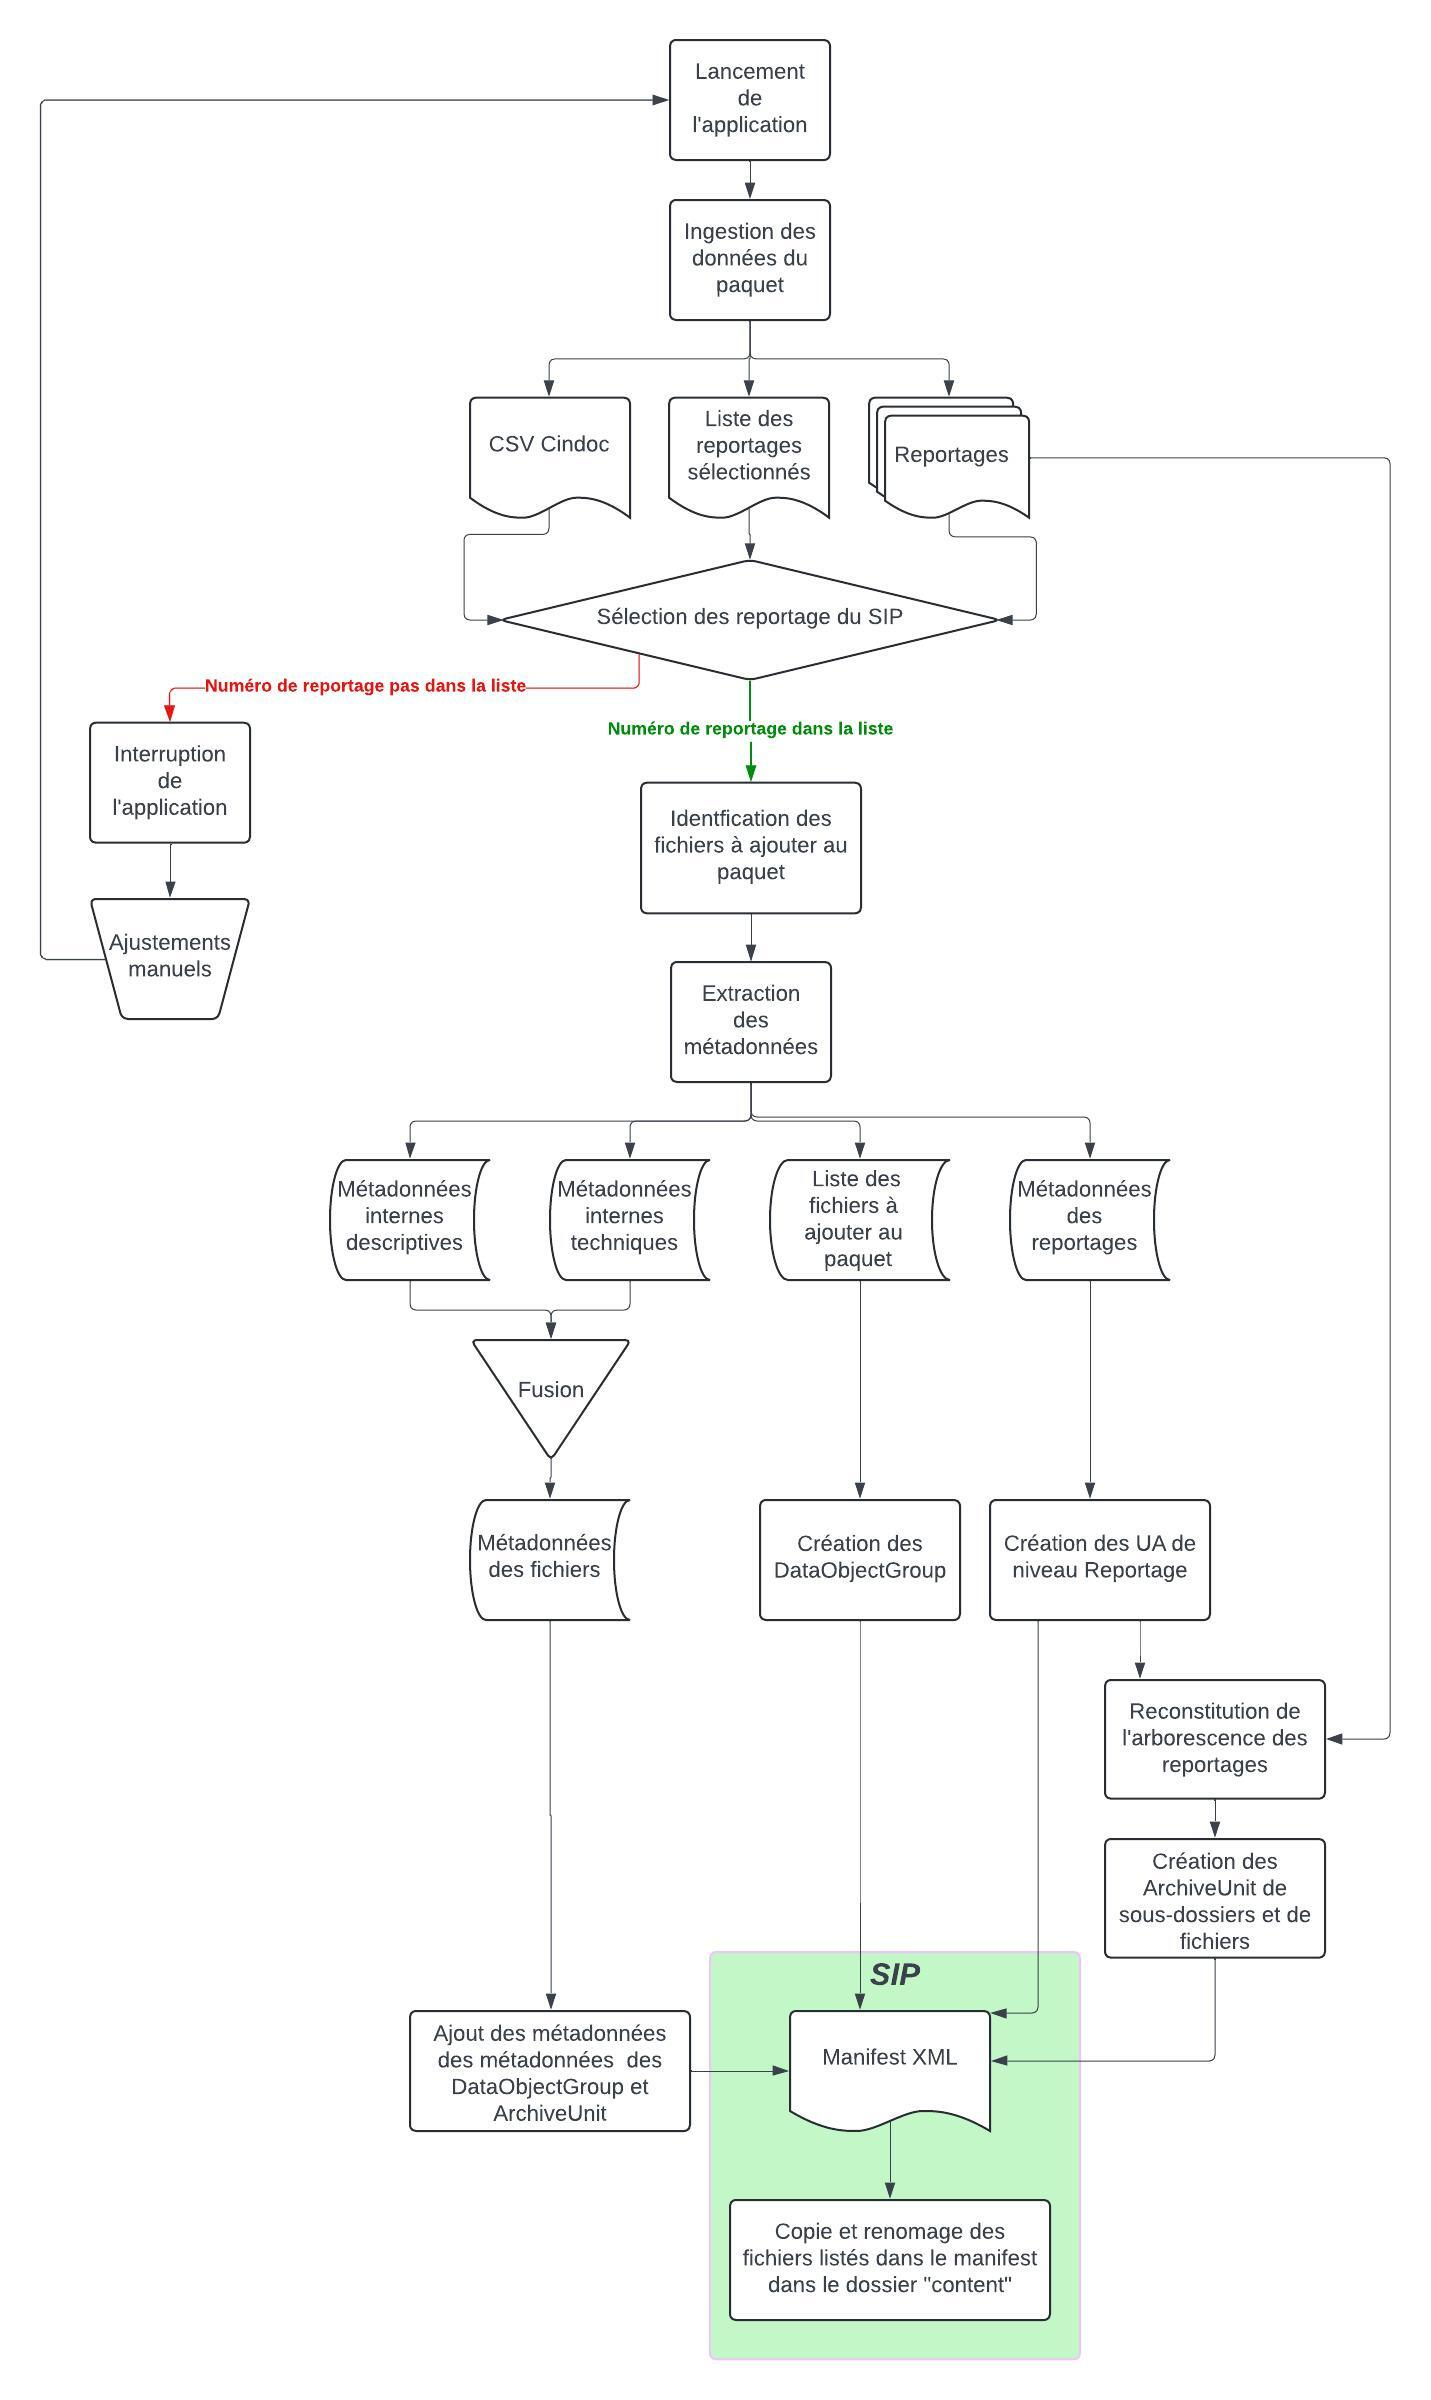
\includegraphics[height=\textheight]{./img/schema_orphee.jpeg}
	\label{fig:schema}
\end{figure}

\chapter[Annexe 2]{Pas à pas pour la fabrication semi-automatique de SIP}
\label{sec:annexe2}
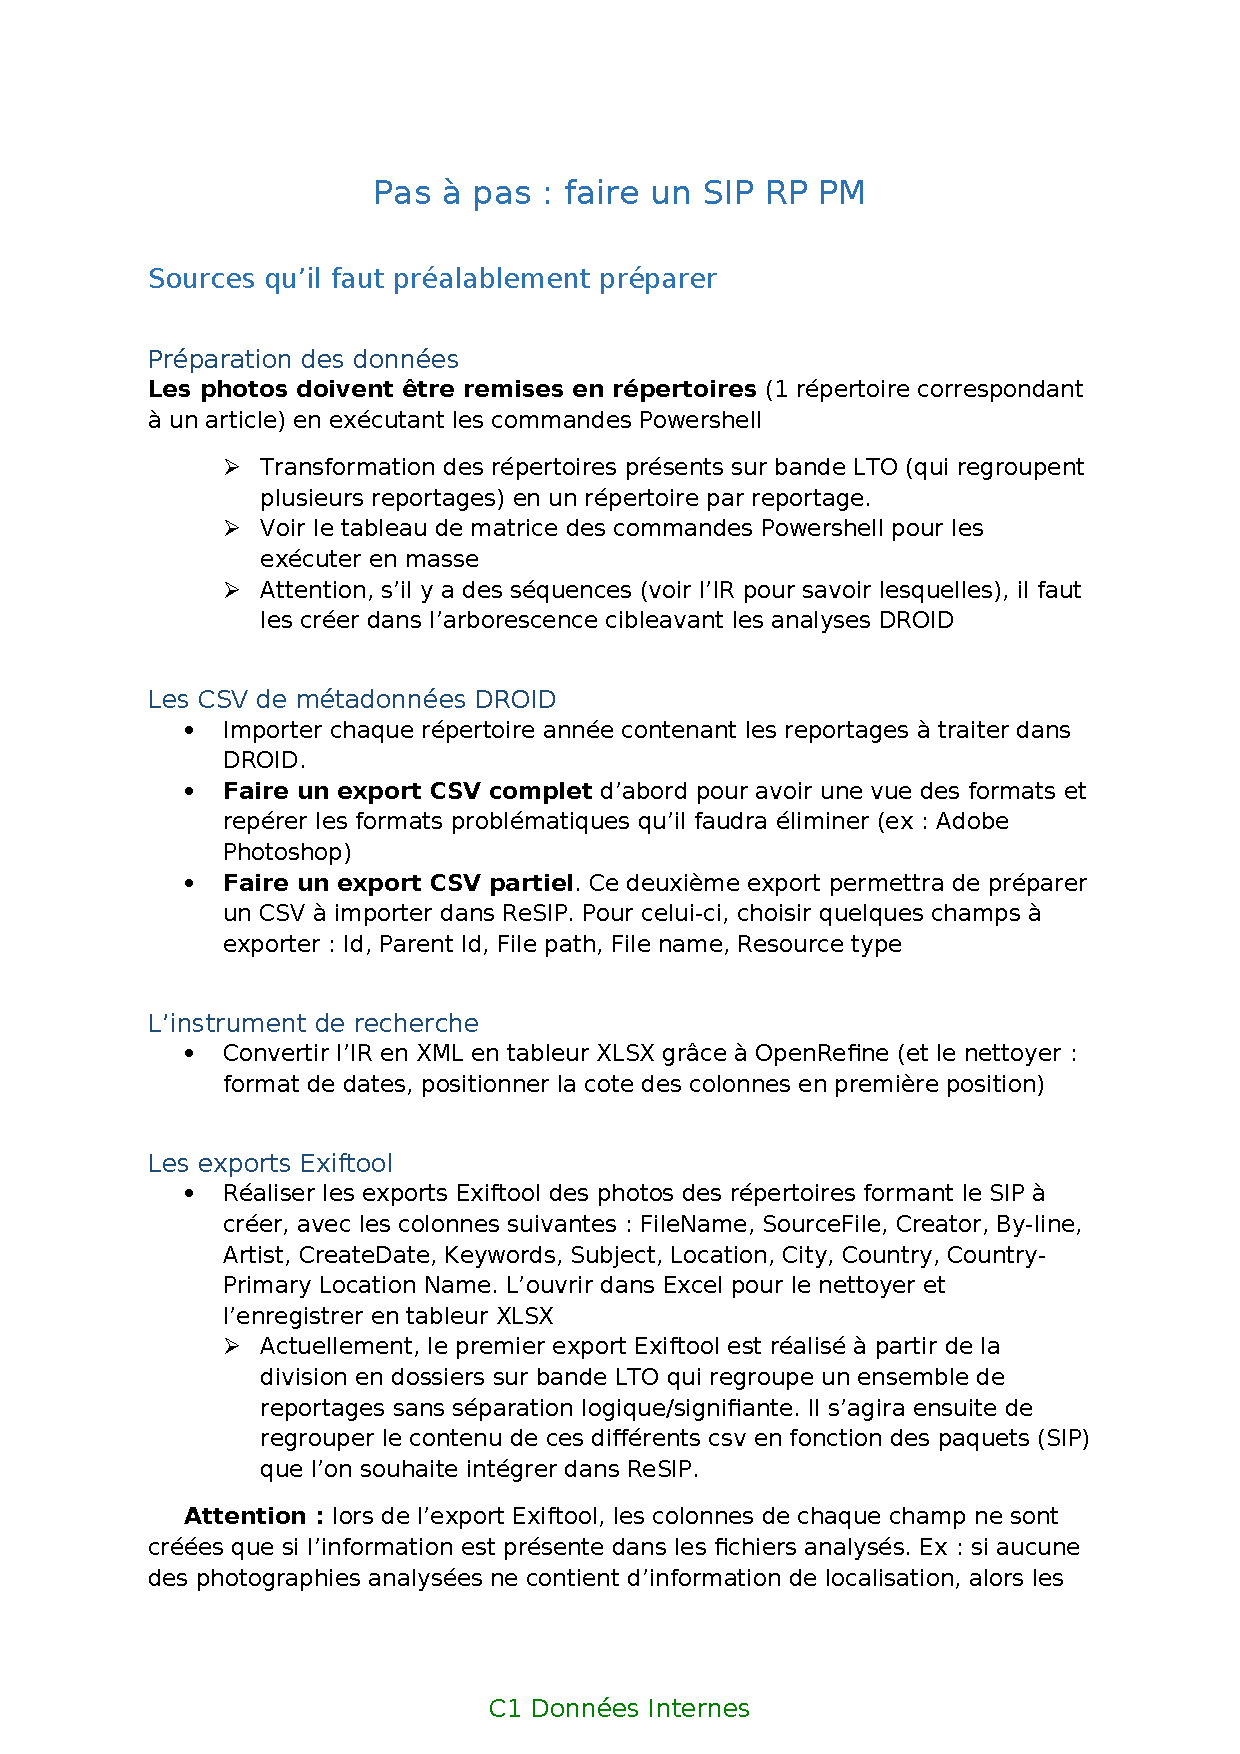
\includepdf[pages=-]{annexe2.pdf}

\newpage{\pagestyle{empty}\cleardoublepage}

%%%%%%%%%%%%%%%%%%

\backmatter 
\printglossaries
\listoftables
\listoffigures
\tableofcontents
\end{document}